%% draft+final=finaldraft (no todos, but draft note at foot of page)
\documentclass[%
    draft, % comment draft to remove draft imprint at page foot
    %final, % give final when done. Overwrites draft. Removes todos.
    11pt,
    a4paper
    %fleqn, %
    %openany %%chapter on right and left pages (no cleardoublepage)
]
{memoir}

\usepackage{blindtext}

%% Prevents figure and table placements in random locations.
\usepackage{float}

\usepackage{hhline}

\usepackage[dvipsnames]{xcolor}
\definecolor{BulletBlue}{HTML}{5783a0}


%% define control flags
\usepackage{ifthen}
\newboolean{printVersion}

\setboolean{printVersion}{false} % do not use colored links for print



\usepackage{lipsum}

%%%%%%%%%%%%%%%%%%%%%%%%%%
%% TOC space settings
%%%%%%%%%%%%%%%%%%%%%%%%%%
\setpnumwidth{3em}
\setrmarg{4em}


%%%%%%%%%%%%%%%%%%%%%%%%%%
%% floating environments
%%%%%%%%%%%%%%%%%%%%%%%%%%
\usepackage[final]          %w/o option final: no images in document-draft-mode
             {graphics}		% einbinden von graphiken

%\usepackage{caption}  %% not needed with documentclass memoir
\usepackage{subcaption} % neue subfigure-Umgebung %% should probably not be used with memoir: generates warning

%\usepackage[section]{placeins} %% \FloatBarrier

%% setup caption style (\usepackage{caption} w/o documentclass memoir)
\captionsetup[figure]{  labelfont       = {bf,color=captionCatergoryColor},
                        textfont        = {it,color=captionTextColor},
                        justification   = raggedright,
                        singlelinecheck = false,
                        position        = bottom,
                        format=hang
                        }
\captionsetup[table]{   labelfont       = {bf,color=captionCatergoryColor},
                        textfont        = {it,color=captionTextColor},
                        justification   = raggedright,
                        singlelinecheck = false,
                        position        = top,
                        format          = hang
                        }
%\captionsetup[table]{skip=7pt} %% mehr platz zwischen tabelle und caption

% move Text to Image. 1ex ~1 line of Text
% unfortunately: also valid for subcaptions.
%\setlength{\belowcaptionskip}{0ex}

% define how much text shall be on same page with large images
%% standard seems to be 0.20 --> 20%
%\renewcommand{\textfraction}{0.01}


%% Durchgängige Nummerierung von Figures und Tables:
%\usepackage{chngcntr}
%\counterwithout{figure}{chapter}
%\counterwithout{table}{chapter}


%define common figure sizes for subfigures
% -> redefined in each environment
\newlength{\subfigureWidth}
\setlength{\subfigureWidth}{0.22\textwidth}
\newlength{\graphicsHeight}
\setlength{\graphicsHeight}{25mm}

%% for page delte (see title-page-tex-file)
%\usepackage{atbegshi}

%%%%%%%%%%%%%%%%%%%%%%%%%%
%% table environments
%%%%%%%%%%%%%%%%%%%%%%%%%%
\usepackage{tabularx}
\newcolumntype{L}[1]{>{\raggedright\arraybackslash}p{#1}} % linksbündig mit Breitenangabe
\newcolumntype{C}[1]{>{\centering\arraybackslash}p{#1}} % zentriert mit Breitenangabe
\newcolumntype{R}[1]{>{\raggedleft\arraybackslash}p{#1}} % rechtsbündig mit Breitenangabe


%% allow multi-row
\usepackage{multirow}
\usepackage{booktabs} %% toprule, midrule and bottomrule for tables



%%%%%%%%%%%%%%%%%%%%%%%%%%
%%for color definitions
%%%%%%%%%%%%%%%%%%%%%%%%%%
\usepackage{xcolor}
%%------------------
%% new colors

% defines the main color theme
% command \colorlet is used to derivate colors from this main color
\definecolor{thesisMainColor}{rgb}{0.36, 0.54, 0.66} %% (92,138,167)@256=100%   #5C8AA7
\definecolor{thesisSecondaryColor}{rgb}{1.00,0.60,0.10} % {cmyk}{0.1, 0.6, 1, 0} %% (255,154,26)@256=100   #FF9A1A

\colorlet{thesisMainColor_dark5}{black!5!thesisMainColor}
\colorlet{thesisMainColor_dark10}{black!10!thesisMainColor}
\colorlet{thesisMainColor_dark15}{black!15!thesisMainColor}
\colorlet{thesisMainColor_dark20}{black!20!thesisMainColor}

% DFKI colors
\definecolor{dfki1}{cmyk}{0.9, 0.55, 0.1, 0}	% DFKI blue
\definecolor{dfki2}{cmyk}{0.1, 0.6, 1, 0}		% DFKI orange
\definecolor{dfki3}{cmyk}{0, 0.89, 0.06, 0.1}	% Magenta Coler Tetrad
\definecolor{dfki4}{cmyk}{0.89, 0, 0.83, 0.1}	% Green Coler Tetrad

\definecolor{grey80}{gray}{0.2}
\definecolor{grey60}{gray}{0.4}
\definecolor{grey40}{gray}{0.6}
\definecolor{grey20}{gray}{0.8}
\definecolor{grey10}{gray}{0.9}



%%------------------
%% derived colors


%chapter numbers
\colorlet{chaptercolor}{thesisMainColor_dark5}

%tables
\colorlet{tableheadingcolor}{thesisMainColor!40}
\colorlet{tablesubheadingcolor}{thesisSecondaryColor!30}

%captions
\colorlet{captionCatergoryColor}{thesisMainColor_dark20}%{grey80!60!thesisMainColor}
\colorlet{captionTextColor}{captionCatergoryColor}%{grey60!60!thesisMainColor}

%itemize
\colorlet{itemicolor}{thesisMainColor_dark5}
\colorlet{itemiicolor}{itemicolor}
\colorlet{itemiiicolor}{itemicolor}

%description text
\colorlet{descriptionColor}{captionCatergoryColor}%{black!20!thesisMainColor}%{thesisMainColor!70!black}%

%footnotes
\colorlet{footnoteMarkColor}{captionCatergoryColor}
\colorlet{footnoteRuleColor}{footnoteMarkColor}
%\colorlet{footnoteTextColor}{footnoteMarkColor} %%not yet needed, color is given by ruleColor


%hyperrefcolors
% we need this switch because of the \refFig etc definitions
\ifthenelse{\boolean{printVersion}}
{%if true
    \colorlet{thesisLinkColor}{black}
    \colorlet{thesisUrlColor}{black}
    \colorlet{thesisCiteColor}{black}
}
{%else
    \colorlet{thesisLinkColor}{captionCatergoryColor}%{black}%{thesisMainColor}%{blue!60!black}
    \colorlet{thesisUrlColor}{thesisMainColor}%{blue!60!black}
    \colorlet{thesisCiteColor}{thesisMainColor}%{thesisSecondaryColor}%{green!60!black}
}


%colors in for acronyms
\colorlet{acroextraColor}{thesisLinkColor}

%color for chapter quotes
\colorlet{quoteColor}{chaptercolor!70!grey80}%{captionTextColor}%

% colors for structure graphs
%% colors for all graph types
\colorlet{structureGraphBgColorMain}{white}%{thesisSecondaryColor!5}%
\colorlet{structureGraphFrameColorMain}{black}%{thesisSecondaryColor!30}%
\colorlet{structureGraphBgColorTitleMain}{grey60}%{thesisSecondaryColor!30}%
\colorlet{structureGraphTextTitleColorMain}{thesisSecondaryColor!80}%{black!50!white}%
\colorlet{structureGraphTextTitleColorBigtopicbox}{white}
%\colorlet{structureGraphContentColor}{thesisMainColor!75} %%not needed, take title_bg_color

%% topic graph
\colorlet{structureGraphBackgroundColorBigtopicbox}{grey20}%{thesisSecondaryColor!5}%
\colorlet{structureGraphFrameColorBigtopicbox}{thesisSecondaryColor!30}%{black!55!white}%
\colorlet{structureGraphTitleBackgroundColorBigtopicbox}{grey40}%{thesisSecondaryColor!45}%

\colorlet{structureGraphBackgroundColorTopicbox}{thesisMainColor!5}
\colorlet{structureGraphFrameColorTopicbox}{thesisMainColor!50}%{thesisSecondaryColor!30}%
\colorlet{structureGraphTitleBackgroundColorTopicbox}{thesisMainColor_dark5}%{thesisMainColor!75}
\colorlet{structureGraphTextTitleColorTopicbox}{thesisMainColor!10}%{white}%{thesisSecondaryColor!30}%

%% chapter graph
\colorlet{structureGraphBackgroundColorChapterbox}{thesisMainColor!1}%{structureGraphBackgroundColorTopicbox}
\colorlet{structureGraphFrameColorChapterbox}{grey40}%{structureGraphFrameColorTopicbox}
\colorlet{structureGraphTitleBackgroundColorChapterbox}{thesisMainColor_dark5}%{structureGraphTitleBackgroundColorTopicbox}
\colorlet{structureGraphTextTitleColorChapterbox}{thesisMainColor!1}%{structureGraphTextTitleColorTopicbox}
 %%own colors with names




%print draft text indo background
\usepackage{rotating}
\usepackage{eso-pic}
%\usepackage{color}
\usepackage{type1cm}

\newcommand{\printdraft}[1][Draft]{
    \AddToShipoutPicture{%
       \AtPageCenter{%\section
         \makebox(0,0){%
           \rotatebox{50}{
               \textcolor[gray]{0.95}{
               		\fontsize{7cm}{7cm}%
               		\selectfont{#1}
                }
            }
          }
        }
    }
}

\usepackage[bookmarks,bookmarksopen=false,bookmarksnumbered=true,pdftex,pdfhighlight=/N,
  linkcolor=thesisLinkColor,%blue!60!black,
  urlcolor=thesisUrlColor,%blue!60!black,
  citecolor=thesisCiteColor,%green!60!black,
  colorlinks=true,
  pdftitle={},
  pdfsubject={},  % insert subtitle
  pdfkeywords={PhD, Multi-Robot System, Wheeled-Leg Rover, SherpaTT, Sherpa},
  pdfauthor={Florian Cordes},
  %final %%use links also in draft mode
  ]{hyperref}


\usepackage{ifdraft} %\ifdraft, \ifoptiondraft, \ifoptionfinal

%% in final document for print: no colored links(?)
\ifdraftdoc
    \hypersetup{final}  %use hyper-final option in draft mode: standard-links
    %\printdraft	        % Print "Draft" Watermark
\else
    %\hypersetup{draft} % use hyper-draft in final document: no links
\fi



%% for faster use of pdflatex
%% DO NOT USE FOR PDF/A compability!
%%\pdfcompresslevel=5
%% check styles/pdf_a_compability.tex





%%%%%%%%%%%%%%%%%%%%%%%%%%
%% setup todo style
%%%%%%%%%%%%%%%%%%%%%%%%%%
%usage: \todo[inline]{blah}
%       \todo{blubb}
\usepackage[obeyFinal]{todonotes}              % todos in text
\presetkeys{todonotes}{fancyline,
                        backgroundcolor=thesisSecondaryColor!50,
                        bordercolor=thesisMainColor,
                        linecolor=thesisMainColor,
                        size=\scriptsize %\footnotesize
                       }{}
\tikzset{/tikz/notestyleraw/.append style={text=thesisMainColor}} % set textcolor
\setlength{\marginparwidth}{2.2cm} % Rand-Notizenbreite einstellen \todo{blahblubb}

\ifdraftdoc
    %%--- define a new todo-list style ---
    \makeatletter
    \def\myaddcontentsline#1#2#3{%
      \addtocontents{#1}{\protect\contentsline{#2}{#3}{\textcolor{thesisMainColor}{\thepage\ ~~ (\textbf{Chapter \thechapter})}}{}}}
    \renewcommand{\@todonotes@addElementToListOfTodos}{%
        \if@todonotes@colorinlistoftodos%
            \myaddcontentsline{tdo}{todo}{{%
                \colorbox{\@todonotes@currentbackgroundcolor}%
                    {\textcolor{\@todonotes@currentbackgroundcolor}{o}}%
                \ \@todonotes@caption}}%
        \else%
            \myaddcontentsline{tdo}{todo}{{\@todonotes@caption}}%
        \fi}%
    \newcommand*\mylistoftodos{%
      \begingroup
           \setbox\@tempboxa\hbox{Chapter 9.9 (p. 999)}%
           \renewcommand*\@tocrmarg{\the\wd\@tempboxa}%
           \renewcommand*\@pnumwidth{\the\wd\@tempboxa}%
           \textcolor{thesisMainColor}{%[rgb]{1.00,0.00,0.00}{
            %\pagecolor{thesisSecondaryColor!50}%
            \begin{small}
                \listoftodos%
            \end{small}
            \todototoc%
            }
        %\clearpage ~~
        %\afterpage{\nopagecolor}
        \clearpage

      \endgroup
    }
    \makeatother
\else
    \newcommand{\mylistoftodos}{}
\fi %end: ifdraftdoc



%%%%%%%%%%%%%%%%%%%%%%%%%%%%
%% page style setup FCordes
%%%%%%%%%%%%%%%%%%%%%%%%%%%%
% ********************************************************************
% composed by Florian Cordes @ DFKI RIC
%
% to be used with documentclass memoir:
% \documentclass[11pt,a4paper]{memoir}
%
% January 2018
% ********************************************************************

\NeedsTeXFormat{LaTeX2e}
\ProvidesPackage{phdDocumentStyle_FCordes}[2018/01/19 v1.0 Style for PhD document]



%Zeilenumbruch, falls overfull hbox
\sloppy
%\relax

%%%%%%%%%%%%%%%%%%%%%%%%%%%%%%%%%%%%%%%%%%%
%% define what happens when
%% draft option is set in documentclass
%%%%%%%%%%%%%%%%%%%%%%%%%%%%%%%%%%%%%%%%%%%
\newcommand{\myDraftNote}[0]{\color{thesisSecondaryColor}{\textit{Draft version: \today}}}
\newcommand{\myFinalDraftNote}[0]{\color{thesisSecondaryColor}{\textit{Final Draft (\today)}}}

\ifdraftdoc
    \makeevenfoot{plain}{}{\thepage}{\myDraftNote}
    \makeoddfoot{plain}{\myDraftNote}{\thepage}{}
    \makeevenfoot{ruled}{\thepage}{}{\myDraftNote}
    \makeoddfoot{ruled}{\myDraftNote}{}{\thepage}
\fi

\makeevenhead{ruled}{\scshape Chapter \leftmark}{}{}
\makeoddhead{ruled}{}{}{\itshape\rightmark}


%%%%%%%%%%%%%%%%
%% Itimisation
%%%%%%%%%%%%%%%%
\newlength{\sqsize}
\setlength{\sqsize}{0.8ex}
\newcommand*\sq{\raisebox{0.4\sqsize}{\rule{\sqsize}{\sqsize}}} % define a small square for itemize bullet

\renewcommand{\labelitemi}{${\color{itemicolor}\sq}$}%\blacksquare}$}
\renewcommand{\labelitemii}{${\color{itemiicolor}\blacktriangleright}$} %\bullet}$}
\renewcommand{\labelitemiii}{${\color{itemiiicolor}\square}$}




%%%%%%%%%%%%%%%%
%% Description
%%%%%%%%%%%%%%%%
\renewcommand*{\descriptionlabel}[1]{\hspace
                                     \labelsep
                                     \normalfont
                                     \textbf{\color{descriptionColor}{#1}}
                                 }




%%%%%%%%%%%%%%%%%%%
%% footnote formatting and colors
%%%%%%%%%%%%%%%%%%%
%change the mark (reference-number)
\renewcommand\thefootnote{\textcolor{footnoteMarkColor}{
                                            (\alph{footnote})%
                                            %\arabic{footnote})%
                                            }}

%change the text at the bottom of the page
\renewcommand{\foottextfont}{\footnotesize}%\color{footnoteTextColor}}

%change the rule above the footnote
\renewcommand*{\footnoterule}{%
    \kern-3pt%
    \color{footnoteRuleColor}\hrule width 0.4\columnwidth %%also sets the text-body color when written like this
    \kern 2.6pt
    }

\setlength{\footnotesep}{2ex}       % the separation between footnotes
\setlength{\footmarkwidth}{1.5em}   % indention of complete footnote textblock
\setlength{\footmarksep}{0.3em}       % indention of second and following lines
\setlength{\footparindent}{2em}     % indention of paragraph within footnote

%make a refernce-command for footnotes
\makeatletter
\newcommand\fnref[1]{\protected@xdef\@thefnmark{\ref{#1}}\@footnotemark}
\makeatother

%do not reset counter per chapter
\counterwithout*{footnote}{chapter}

% footnotes shall be at the bottom of the page, even wenn a figure has [b] option
\feetbelowfloat

%%%%%%%%%%%%%%%%%%%%%%%%%%%%%%
%% Define sectioning depth
%%%%%%%%%%%%%%%%%%%%%%%%%%%%%%
\setsecnumdepth{subsection}
\settocdepth{section}


%%%%%%%%%%%%%%%%%%%%%%%%%%%%%%
%% new line spacing
%%%%%%%%%%%%%%%%%%%%%%%%%%%%%%
\setSingleSpace{1.05}
\SingleSpacing





%%%%%%%%%%%%%%%%%%%%%%%%%%%%%%%%%%%%%%%%%%%
%% define the text field for the pages
%%%%%%%%%%%%%%%%%%%%%%%%%%%%%%%%%%%%%%%%%%%
\newlength{\myRegularParskip}
\setlength{\myRegularParskip}{1.8mm}

\newlength{\myCenterSpaceOffset}
\setlength{\myCenterSpaceOffset}{0.7mm} % pos increases spacing in center of double page

\textheight235mm              % Höhe des Textbereichs
\textwidth160mm             % Breite des Textbereichs
\topmargin-20mm
\topskip5mm
\headheight20mm
\headsep3mm
\setlength\evensidemargin{-\myCenterSpaceOffset} % pos vals to move in
\setlength\oddsidemargin{\myCenterSpaceOffset}   % neg vals to move in
\footskip15mm
\headwidth\textwidth

\setlength\parindent{0mm}
\setlength\parskip{\myRegularParskip}


%%%%%%%%%%%%%%%%%%%%%%%%%%%%%%
%% Defines for Chapter Style
%%%%%%%%%%%%%%%%%%%%%%%%%%%%%%
\usepackage{kpfonts}

\newcommand\numlifter[1]{\raisebox{-2.5cm}[0pt][0pt]{\smash{#1}}} % how low can you go?
\newcommand\numindent{\kern10pt} %space from right margin
\newlength\chaptertitleboxheight
\makechapterstyle{cordesDiss}{
  \renewcommand\printchaptername{\raggedleft}
  \renewcommand\printchapternum{%
    \begingroup%
    \leavevmode%
    \chapnumfont%
    \strut%
    \numlifter{\thechapter}%{\fontfamily{pnc}\selectfont \thechapter} }%
    \numindent%
\endgroup%
}
  \renewcommand*{\printchapternonum}{%
    \vphantom{\begingroup%
      \leavevmode%
      \chapnumfont%
      \numlifter{\vphantom{9}}%
      \numindent%
      \endgroup}
    \afterchapternum}
  \setlength\midchapskip{0pt}
  \setlength\beforechapskip{0.5\baselineskip}
  \setlength{\afterchapskip}{3\baselineskip}
  \renewcommand\chapnumfont{%
    \fontsize{4cm}{0cm}%
    \bfseries%
    \sffamily%
    \color{chaptercolor}%
  }
  \renewcommand\chaptitlefont{%
    \normalfont%
    \huge%
    \bfseries%
    \raggedleft%
  }%
  \settototalheight\chaptertitleboxheight{%
    \parbox{\textwidth}{\chaptitlefont \strut bg\\bg\strut}}
  \renewcommand\printchaptertitle[1]{%
    \parbox[t][\chaptertitleboxheight][t]{\textwidth}{%
      %\microtypesetup{protrusion=false}% add this if you use microtype
      \chaptitlefont\fontsize{0.9cm}{\baselineskip}\selectfont\strut ##1\strut}%FC
      %\chaptitlefont \strut ##1\strut}% ORIGINAL
      %\HUGE\bfseries\strut ##1\strut}% FC
}}

%% now set the style active
\chapterstyle{cordesDiss}
\aliaspagestyle{chapter}{plain} % just to save some space: no header

%\createplainmark{toc}{both}{\acronym}


%% -----------------------------
%% floating environment options
%% -----------------------------

% define how much text shall be on same page with large images
%% standard seems to be 0.20 --> 20%
%\renewcommand{\textfraction}{0.01}


%% setup caption style
\captionsetup[figure]{labelfont={bf,color=captionCatergoryColor},textfont={it,color=captionTextColor},justification=raggedright,singlelinecheck=false,format=hang}
\captionsetup[table]{labelfont={bf,color=captionCatergoryColor},textfont={it,color=captionTextColor},justification=raggedright,singlelinecheck=false,format=hang}
%\captionsetup[table]{skip=7pt} %% mehr platz zwischen tabelle und caption

%% Durchgängige Nummerierung von Figures und Tables:
%\usepackage{chngcntr}
%\counterwithout{figure}{chapter}
%\counterwithout{table}{chapter}



%% --------------------
%% special functions
%% --------------------

% acronym
\newcommand{\dissAcroextra}[1]{\acroextra{~\\[-0.6ex]\textcolor{acroextraColor}{\scriptsize{(#1)}}}}

% quote at beginning of chapter
\newcommand{\shinyChapterQuote}[2]{
\begin{quote}\hypersetup{hidelinks=true}
    \textcolor{quoteColor}{
        \emph{#1}
        \newline\indent\qquad -- #2
    }
\end{quote}
}

% a command to add (smaller) extra info in captions of Figures and Tables
\newcommand{\dissExtraCaption}[1]{\newline\footnotesize{#1}}

%% symbols
\newcommand{\dissCheck}{\textcolor{thesisMainColor}{$\mathbf{\checkmark}$}}
\newcommand{\dissUncheck}{\textcolor{thesisSecondaryColor}{$\mathbf{\times}$}}
\newcommand{\myTTAmark}{\textcolor{thesisSecondaryColor!80}{\ensuremath{^\star}}\xspace}%{\ensuremath{^\circledast}}\xspace}%{\ensuremath{^\blacklozenge}}\xspace}



%%%%%%%%%%%%%%%%%%%%%%%%%%
%% define the boxes for thesis structure graph
%%%%%%%%%%%%%%%%%%%%%%%%%%


%
% use as option in tcolorbox environment:
% [code={\pgfkeysalsofrom{\outerboxoptions}}, otheroption=...]
%
\def\outerboxoptions{ %the thesis frame
    colback=structureGraphBackgroundColorBigtopicbox,%grey10,%structureGraphBgColorMain,
    colframe=structureGraphFrameColorBigtopicbox,%structureGraphFrameColorMain,
    colbacktitle=structureGraphTitleBackgroundColorBigtopicbox,%structureGraphBgColorTitleMain,
    coltitle=thesisMainColor!50!black,%structureGraphTextTitleColorMain,
    left=1mm,
    right=1mm,
    boxrule=0.8pt
}

\def\topicboxoptions{
    %sidebyside,righthand width=.26\textwidth,
    colback=structureGraphBgColorMain,
    colframe=structureGraphFrameColorMain,
    colbacktitle=structureGraphBgColorTitleMain,
    coltitle=structureGraphTextTitleColorMain,
    boxrule=0.8pt,
    left=1mm,
    right=1mm
}


\def\chapterboxoptions{
    colback=structureGraphBackgroundColorChapterbox,
    colframe=structureGraphFrameColorChapterbox,
    colbacktitle=structureGraphTitleBackgroundColorChapterbox,
    coltitle=structureGraphTextTitleColorChapterbox,
    boxrule=0.6pt,
    left=0.6mm,
    right=0.6mm,
    top=1mm,
    bottom=1mm
    %drop large lifted shadow,
}

\def\outerrasteroptions{
    raster width=\linewidth,
    raster columns=1,
    %% Forces same height in all columns on same row
    raster equal height=rows,
    raster every box/.style={valign=center, halign=center}
}

\def\innerrastersinglecoloptions{
    raster columns=1,
    raster width=0.5\linewidth, %otherwise inherits from outer raster
    %% Forces same height in all columns on same row
    raster equal height=rows,
    raster every box/.style={valign=center, halign=center},
}

\def\innerrasterdualcoloptions{
    raster columns=2,
    raster width=0.992\linewidth, %otherwise inherits from outer raster
    %% Forces same height in all columns on same row
    raster equal height=rows,
    raster every box/.style={valign=center, halign=center},
}

\def\innerrastertriplecoloptions{
    raster columns=3,
    raster width=0.992\linewidth, %otherwise inherits from outer raster
    %% Forces same height in all columns on same row
    raster equal height=rows,
    raster every box/.style={valign=center, halign=center},
}









\newcommand{\drawChapterbox}[2]{
    %\begingroup
        \hypersetup{hidelinks=true}%
        \begin{tcolorbox}[code={\pgfkeysalsofrom{\chapterboxoptions}},
                          title=\structuregraphChapterName{#1}]
            \flushleft{
                \footnotesize{\color{thesisCiteColor}{#2}}%
            }%
        \end{tcolorbox}%
    %\endgroup
}


%% use this (and make according commands for the other boxes) 
%% if you do not want to use citations in the graph:
%% leave it at to input-vals to be compatible.
%\newcommand{\drawChapterbox}[2]{
%    %\begingroup
%        \hypersetup{hidelinks=true}%
%        \begin{tcolorbox}[code={\pgfkeysalsofrom{\chapterboxoptions}},
%                          title=\textbf{\small{Chapter~\ref{#1}}}]
%            \flushleft{
%                \footnotesize{\color{thesisCiteColor}{\nameref{#1}}}%
%            }%
%        \end{tcolorbox}%
%    %\endgroup
%}


\newcommand{\drawChapterboxSota}[2]{
    %\begingroup
        \hypersetup{hidelinks=true}%
        \begin{tcolorbox}[code={\pgfkeysalsofrom{\chapterboxoptions}},
                          title=\footnotesize{\textbf{Chapter~\ref{#1}}~\\[0.5ex]\nameref{#1} \newline\rule{0mm}{4.5mm}}]
            \flushleft{
                \footnotesize{\color{thesisCiteColor}{#2}}%
            }%
        \end{tcolorbox}%
    %\endgroup
}

\newcommand{\drawAppendixbox}[2]{
    %\begingroup
        \hypersetup{hidelinks=true}%
        \begin{tcolorbox}[code={\pgfkeysalsofrom{\chapterboxoptions}},
                          width=0.3\linewidth,
                          %drop large lifted shadow,
                          title=\structuregraphAppendixName{#1}]
            \flushleft{
                \footnotesize{\color{thesisCiteColor}{#2}}%
            }%
        \end{tcolorbox}%
    %\endgroup
}






% command for identical newline space between different boxes
\newcommand{\structuregraphNewline}{~\\[3ex]}

% command for Part captions
\newcommand{\structuregraphPartCaption}[1]{
    \Large
        ~\\ %% some extra space to separate Part-Header from chapters before
        \textbf{Part~\ref{#1}}~\\[2ex]
    \normalsize
}

% command for the basic info in each box (w/o the cites)
\newcommand{\structuregraphChapterName}[1]{
    %\color{structureGraphSectionColor}{
    \footnotesize{
        \textbf{Chapter~\ref{#1}}~\\[0.5ex]
        \nameref{#1}
        }
    %}%
}

% command for the basic info in each box (w/o the cites)
\newcommand{\structuregraphAppendixName}[1]{
    %\color{structureGraphSectionColor}{
    \footnotesize{
        \textbf{Appendix~\ref{#1}}~\\[0.5ex]%~\ref{#1}}~\\[0.5ex]
        \nameref{#1}
        }
    %}%
}


\newcommand{\partbox}[3]{
    \begin{tcolorbox}[enhanced,
                      sidebyside,
                      comment outside listing,
                      lefthand width=8mm,
                      title=#1,
                      boxsep=-0.5pt,
                      bottom=1.5mm,
                      left=1.5mm,
                      right=2.5mm,
                      top=1.5mm,
                      boxrule=0.5pt,
                      colframe=descriptionColor,
                      %lower separated=false, % no separation line
                      notitle,
                      ]
        \rotatebox{90}{\textcolor{descriptionColor}{#1}}
        \rotatebox{90}{\textcolor{descriptionColor}{#2}}
         \tcblower
         #3
    \end{tcolorbox}
}





%%%%%%%%%%%%%%%%%%%%%%%%%%%
%% cumlative PhD functions
%%%%%%%%%%%%%%%%%%%%%%%%%%%
% a package for including the publications pdfs
%%%-------------------------------------------------------------------------------
%% a style package for cumulative dissertations
%% provides funtions for ease of appending pdf publications
%%
%% author: Florian Cordes
%% date:   2018-03-07
%%-------------------------------------------------------------------------------

\NeedsTeXFormat{LaTeX2e}

\usepackage{etoolbox}
\usepackage[final]{pdfpages} %%including compiled pdf files in document

%% make a new page style, initially copy from ruled
\copypagestyle{pubsAppendix}{ruled}

%%define commands for publication info
\newcommand{\pubTitle}{[nan] \textbf{dummy title}}
\newcommand{\pubAuthors}{\emph{Author}}
\newcommand{\pubPlace}{where published}

\newcommand{\pubInfo}{\scriptsize \pubTitle~\\  \pubAuthors~\\  in: \pubPlace}


\makeevenhead{pubsAppendix}{}{\pubInfo}{}
\makeoddhead{pubsAppendix}{}{\pubInfo}{}
%%leave footer as copied from original style
%\makeevenfoot{pubsAppendix}{left}{center}{right}
%\makeoddfoot{pubsAppendix}{left}{center}{right}


%% commands for bibkey list
\newcounter{bibkeycnt}
\newcommand\setbibkey[2]{%
  \csdef{bibkey#1}{#2}%
}
\newcommand\addbibkey[1]{%
    \stepcounter{bibkeycnt}%
    \csdef{bibkey\thebibkeycnt}{#1}
}
\newcommand\getbibkey[1]{%
      \csuse{bibkey#1}%
}

%% commands for title list
\newcounter{titlecnt}
\newcommand\settitle[2]{%
  \csdef{title#1}{#2}%
}
\newcommand\addtitle[1]{%
    \stepcounter{titlecnt}%
    \csdef{title\thetitlecnt}{#1}
}
\newcommand\gettitle[1]{%
      \csuse{title#1}%
}

%% commands for authors list
\newcounter{authorscnt}
\newcommand\setauthors[2]{%
  \csdef{authors#1}{#2}%
}
\newcommand\addauthors[1]{%
    \stepcounter{authorscnt}%
    \csdef{authors\theauthorscnt}{#1}
}
\newcommand\getauthors[1]{%
      \csuse{authors#1}%
}


%% commands for place list
\newcounter{placecnt}
\newcommand\setplace[2]{%
  \csdef{place#1}{#2}%
}
\newcommand\addplace[1]{%
    \stepcounter{placecnt}%
    \csdef{place\theplacecnt}{#1}
}
\newcommand\getplace[1]{%
      \csuse{place#1}%
}

%% commands for copyright list
\newcounter{copyrgtcnt}
\newcommand\setcopyrgt[2]{%
  \csdef{copyrgt#1}{#2}%
}
\newcommand\addcopyrgt[1]{%
    \stepcounter{copyrgtcnt}%
    \csdef{copyrgt\thecopyrgtcnt}{#1}
}
\newcommand\getcopyrgt[1]{%
      \csuse{copyrgt#1}%
}

%% commands for internetlink list
\newcounter{urllinkcnt}
\newcommand\seturllink[2]{%
  \csdef{urllink#1}{#2}%
}
\newcommand\addurllink[1]{%
    \stepcounter{urllinkcnt}%
    \csdef{urllink\theurllinkcnt}{#1}
}
\newcommand\geturllink[1]{%
      \csuse{urllink#1}%
}






%% this constructes the header and includes the pdf file (name should be the same as the bib key
\newcommand{\includeAccuPub}[1]{
    \renewcommand{\pubTitle}{\citeown{\getbibkey{#1}}: \textbf{\gettitle{#1}}}
    \renewcommand{\pubAuthors}{\emph{\getauthors{#1}}}
    \renewcommand{\pubPlace}{\getplace{#1}}

    \renewcommand{\pubInfo}{\scriptsize  \pubTitle~\\  \pubAuthors~\\ in: \pubPlace \quad \getcopyrgt{#1}}

    \addcontentsline{toc}{section}{[#1] -- \gettitle{#1}}%\pubTitle}
    \ifthenelse{\boolean{printVersion}}
    {%if true: include greyscale publications
        \includepdf[pages=-,scale=0.8,frame=true,offset=0cm 0.0cm,pagecommand={\pagestyle{pubsAppendix}}]{publications/\getbibkey{#1}_bw.pdf}
    }
    {%else: include color publications
        \includepdf[pages=-,scale=0.8,frame=true,offset=0cm 0.0cm,pagecommand={\pagestyle{pubsAppendix}}]{publications/\getbibkey{#1}.pdf}
    }
    
    \cleardoublepage %start each paper on right page. Leave left page blank/no header or footer
}



%%%%%%%%%%%%%%%%%%%%%%%%%%
%% miscellaneous packages
%%%%%%%%%%%%%%%%%%%%%%%%%%
\usepackage[utf8]{inputenc}

\usepackage{tabto} %%something like a tabstop: required for usage in itemize

\usepackage{moreverb}
\usepackage{ifthen}     % Programmierkonstrukte

\usepackage{textcmds} %% quotation marks with \qq{my text} \q{my text}
\usepackage{xspace}

\usepackage[per=fraction,separate-uncertainty=true,multi-part-units=single,round-mode=places,round-precision=1]{siunitx}


\usepackage{paralist}    % for compact item

%\usepackage{relsize}
\usepackage[%nolist,         %% no listing for acronyms
            printonlyused,  %% print only the used ones, not the full list
            %smaller        %% to be a bit smaller in text (needs relsize package)
            ]
            {acronym}


\usepackage{afterpage}

\usepackage{forloop}


%%%%%%%%%%%%%%%%%%%%%%%%%%
%% math stuff
%%%%%%%%%%%%%%%%%%%%%%%%%%
\usepackage{amsmath}
\usepackage{amsfonts}
\usepackage{amssymb}
\usepackage{array}



%%%%%%%%%%%%%%%%%%%%%%%%%%
%% structure graphs
%%%%%%%%%%%%%%%%%%%%%%%%%%
\usepackage[most]{tcolorbox} %% colored boxes
\usepackage{colortbl}   %%colored tables


%%define the citations contributing to a chapter
%%% shortcuts for the citations per chapter (re-usable in front of each chapter)
%% use list of \citeown{} commands per chapter
\newcommand{\introCites}[0]{
    ~\xspace
}

\newcommand{\sotaCites}[0]{
    \citeown{myPubA} %
    \citeown{myPubB} %
    \xspace
}


\newcommand{\designCites}[0]{
    \citeown{myPubB} %
    \citeown{myPubC} %
    \xspace
}

\newcommand{\controlCites}[0]{
    \citeown{myPubB} %
    \citeown{myPubC} %
    \xspace
}

\newcommand{\expCites}[0]{
    \citeown{myPubC} %
    \xspace
}

\newcommand{\conclusionCites}[0]{
    ~\xspace
}

\newcommand{\AppACites}[0]{
    ~\xspace
}


\newlength{\pubsItemSep}
\setlength{\pubsItemSep}{0em}
\newlength{\pubsTopSep}
\setlength{\pubsTopSep}{0em}



\newcommand{\chapterSupportedBy}[1]{
    %This chapter is supported by the following publications:
    The following publications contribute to the contents of this chapter:
    %\begin{quote}
    %\begin{footnotesize}
    \begin{small}
    #1
    \end{small}
    \clearpage
    %\end{footnotesize}
    %\end{quote}
}


\newcommand{\sotaCitesLong}[0]{
    \begin{itemize}
    \setlength\itemsep{\pubsItemSep}
    \setlength\topsep{\pubsTopSep}
        \item[\citeown{myPubA}]
            \textbf{%
                My Glorious Publication A%
            };
            \textit{Some Author, Another Author, Me}; Journal of Field Robotics, 2075.
        \item[\citeown{myPubB}] \textbf{Yet Another Fantastic Publication}; \textit{Me, Author Numbertwo}; Journal of Intelligent Service Robotics, 2039.
    \end{itemize}
}




\newcommand{\designCitesLong}[0]{
    \begin{itemize}
    \setlength\itemsep{\pubsItemSep}
     \setlength\topsep{\pubsTopSep}
        \item[\citeown{myPubB}] \textbf{Yet Another Fantastic Publication}; \textit{Me, Author Numbertwo}; Journal of Intelligent Service Robotics, 2039.
        \item[\citeown{myPubC}] \textbf{Final Experiment Result Paper of Great Importance}; \textit{Me, Author Numbertwo, Prof. XYZ}; Science, 2090.
    \end{itemize}
}


\newcommand{\controlCitesLong}[0]{
    \begin{itemize}
    \setlength\itemsep{\pubsItemSep}
     \setlength\topsep{\pubsTopSep}
        \item[\citeown{myPubB}] \textbf{Yet Another Fantastic Publication}; \textit{Me, Author Numbertwo}; Journal of Intelligent Service Robotics, 2039.
        \item[\citeown{myPubC}] \textbf{Final Experiment Result Paper of Great Importance}; \textit{Me, Author Numbertwo, Prof. XYZ}; Science, 2090.
    \end{itemize}
}

\newcommand{\expCitesLong}[0]{
    \begin{itemize}
    \setlength\itemsep{\pubsItemSep}
     \setlength\topsep{\pubsTopSep}
        \item[\citeown{myPubC}] \textbf{Final Experiment Result Paper of Great Importance}; \textit{Me, Author Numbertwo, Prof. XYZ}; Science, 2090.
    \end{itemize}
}






%%%%%%%%%%%%%%%%%%%%%%%%%%
%% bib setup
%%%%%%%%%%%%%%%%%%%%%%%%%%
% two separate bibs
\usepackage{multibib}
\newcites{sota,own}%
         {Literature References,Own Publications}%
\bibliographystylesota{apalike}%{alpha}
\bibliographystyleown{ieeetr}%{unsrt}%{plain}






%%hyphenation
\hyphenation{every-where}
\hyphenation{re-con-fi-gu-rable}

%% toc "Parts"
\newcommand{\addTocCaption}[1]{%
    \cftaddtitleline{toc}{chapter}{\vspace{-0.2cm}}{} %extra space before caption
    \cftaddtitleline{toc}{chapter}{\centerline{\rule{20mm}{0.2mm}~~\textsc{\Large{#1}}~~\rule{20mm}{0.2mm}}\vspace{-0.2cm}}{}%
}

\newcommand{\addTocPubEntry}[1]{%
    \cftaddtitleline{toc}{section}{[#1] -- \gettitle{#1} \hfill\hfill\hfill\hfill\hfill\hfill\hfill\hfill\hfill\hfill\hfill\hfill\hfill\hfill\hfill\hfill\hfill\hfill\hfill\hfill}{}
    \cftaddtitleline{toc}{chapter}{\vspace{-0.75cm}}{} % more spacing after entry
}

%% referencing stuff
\newcommand{\refFig}[1]{\textcolor{thesisLinkColor}{Figure}~\ref{#1}}
\newcommand{\refTab}[1]{\textcolor{thesisLinkColor}{Table}~\ref{#1}}
\newcommand{\refChpt}[1]{\textcolor{thesisLinkColor}{Chapter}~\ref{#1}}
\newcommand{\refSec}[1]{\textcolor{thesisLinkColor}{Section}~\ref{#1}}
\newcommand{\refSubSec}[1]{\textcolor{thesisLinkColor}{Subsection}~\ref{#1}}
\newcommand{\refApp}[1]{\textcolor{thesisLinkColor}{Appendix}~\ref{#1}}
\newcommand{\refEqn}[1]{\textcolor{thesisLinkColor}{Equation\,(\ref{#1})}}
\newcommand{\refPage}[1]{\textcolor{thesisLinkColor}{Page\,\pageref{#1}}}
\newcommand{\refToAccumulatedPubs}{\textcolor{thesisLinkColor}{Appendix}~\ref{sec:AccumulatedPublications} -- \nameref{sec:AccumulatedPublications}\xspace}


%% how software commands are formatted within text:
\newcommand{\swCmd}[1]{\texttt{#1}}



%% other names
\newcommand{\ftsensor}{force/torque sensor\xspace}
\newcommand{\Ftsensor}{Force/torque sensor\xspace} %new sentence
\newcommand{\ftsensors}{force/torque sensors\xspace}
\newcommand{\Ftsensors}{Force/torque sensors\xspace} %new sentence
\newcommand{\icH}{iC-Haus\xspace}
\newcommand{\eg}{e.g.\;} %
\newcommand{\ie}{i.e.\;} %
\newcommand{\cf}{cf.\;} %
\newcommand{\wrt}{with respect to\xspace}%{w.r.t.\;}

\newcommand{\etal}{et.\,al.}

\newcommand{\x}{\ensuremath{\times}}

\newcommand{\dg}{\ensuremath{^\circ}\xspace}
\newcommand{\uC}{\ensuremath{\mu}C\xspace}
\newcommand{\Ohm}{\ensuremath{\Omega}\xspace}


%% greek symbols
%\newunicodechar{ɑ}{\ensuremath{\alpha}}
%\newunicodechar{β}{\ensuremath{\beta}}

%% shortcuts (removed from acronyms)
\newcommand{\SOTA}{state of the art\xspace}
\newcommand{\SoS}{system of systems\xspace}
\newcommand{\OBC}{on board computer\xspace}
\newcommand{\HD}{HD\xspace}
\newcommand{\MAV}{mars ascend vehicle\xspace}
\newcommand{\PMS}{power management system\xspace}
\newcommand{\INC}{internal communication\xspace}
\newcommand{\LOC}{local communication\xspace}
\newcommand{\GLC}{global communication\xspace}
%\newcommand{\PSR}{\ac{PSR}\xspace}
%\newcommand{\PSRs}{\acp{PSR}\xspace}
\newcommand{\CAD}{CAD\xspace}

\newcommand{\fromFirstToLastPub}{[\textcolor{thesisCiteColor}{1}] - [\textcolor{thesisCiteColor}{13}]\xspace}

\newcommand{\massSherpaTT}{170\,kg\xspace}


%% common phrases
\newcommand{\elecmech}{electromechanical\xspace}
\newcommand{\electromech}{\elecmech} %synonym
\newcommand{\elecmechly}{electromechanically\xspace}
\newcommand{\Elecmech}{Electromechanical\xspace}
\newcommand{\ElecMech}{Electromechanical\xspace}%{Electro-Mechanical\xspace}

%% units
\newcommand{\unitmm}{\text{\,mm}\xspace}
\newcommand{\unitmeter}{\text{\,m}\xspace}
\newcommand{\unitm}{\unitmeter}
\newcommand{\unitkg}{\text{\,kg}\xspace}
\newcommand{\unitcubmeter}{\text{\,m\ensuremath{^3}}\xspace}
\newcommand{\unitNewton}{\text{\,N}\xspace}
\newcommand{\unitN}{\unitNewton}
\newcommand{\unitsecond}{\text{\,s}\xspace}
\newcommand{\units}{\unitsecond}
\newcommand{\unitmpersec}{\,\text{m/s}\xspace}
\newcommand{\unitdegpersec}{\,\text{deg/s}\xspace}
\newcommand{\unitW}{\,\text{W}\xspace}


%% math stuff
% to make greek letters bold
\usepackage{bm}
\newcommand*{\B}[1]{\ifmmode\bm{#1}\else\textbf{#1}\fi}

% atan2
\newcommand{\atant}{\arctan\!2\xspace}

%notation of vector symbols (can be bold or with arrow on top etc...)
\newcommand{\myVec}[1]{\ensuremath{\B{#1}}} %% vector notation in text
\newcommand{\myVecSub}[2]{\ensuremath{\myVec{#1}_{#2}}} %% vector notation with subscript in text
\newcommand{\myVecSup}[2]{\ensuremath{\myVec{#1}^{#2}}} %% vector notation with subscript in text
\newcommand{\myVecSubSup}[3]{\ensuremath{\myVec{#1}_{#2}^{#3}}} %% vector notation with subscript and superscript in text


%alias for matrices. can be changed later to different style if required
\newcommand{\myMat}[1]{\myVec{#1}}
\newcommand{\myMatSub}[2]{\myVecSub{#1}{#2}}
\newcommand{\myMatSup}[2]{\myVecSup{#1}{#2}}
\newcommand{\myMatSubSup}[3]{\myVecSubSup{#1}{#2}{#3}}


% stacked vectors in math environment
\newcommand{\vekk}[2]{\begin{pmatrix} #1\\ #2 \end{pmatrix}}
\newcommand{\vekkk}[3]{\begin{pmatrix} #1\\ #2\\ #3\end{pmatrix}}
\newcommand{\vekkkk}[4]{\begin{pmatrix} #1\\ #2\\ #3\\ #4\end{pmatrix}}
\newcommand{\vekkkkkk}[6]{\begin{pmatrix} #1\\ #2\\ #3\\ #4\\ #5\\ #6 \end{pmatrix}}

%%%----------------------formula text functions---------------------------------%%%
\newcommand{\ftf}[1]{\begin{array}[c]{l}  \text{\footnotesize{#1}} \end{array}}  % Formeltext 1Zeile, footnotesize                                                                                      % Formeltext 1Zeile, footnotesize
\newcommand{\ftff}[2]{\begin{array}[c]{l} \text{\footnotesize{#1}}\\
                                          \text{\footnotesize{#2}}\end{array}}  % Formeltext 2Zeilen, footnotesize
\newcommand{\ftfff}[3]{\begin{array}[c]{l}\text{\footnotesize{#1}}\\
                                          \text{\footnotesize{#2}}\\
                                          \text{\footnotesize{#3}}\end{array}}  % Formeltext 3Zeilen, footnotesize
\newcommand{\ftffff}[4]{\begin{array}[c]{l}\text{\footnotesize{#1}}\\
                                          \text{\footnotesize{#2}}\\
                                          \text{\footnotesize{#3}}\\
                                          \text{\footnotesize{#4}}\end{array}}  % Formeltext 4Zeilen, footnotesize
\newcommand{\ftfffff}[5]{\begin{array}[c]{l}\text{\footnotesize{#1}}\\
                                          \text{\footnotesize{#2}}\\
                                          \text{\footnotesize{#3}}\\
                                          \text{\footnotesize{#4}}\\
                                          \text{\footnotesize{#5}}\end{array}}  % Formeltext 5Zeilen, footnotesize
\newcommand{\ftffffff}[6]{\begin{array}[c]{l}\text{\footnotesize{#1}}\\
                                          \text{\footnotesize{#2}}\\
                                          \text{\footnotesize{#3}}\\
                                          \text{\footnotesize{#4}}\\
                                          \text{\footnotesize{#5}}\\
                                          \text{\footnotesize{#6}}\end{array}}  % Formeltext 6Zeilen, footnotesize 


% if both, draft, final are set, we get the draft note at the bottom of a page
\ifoptionfinal{
    \ifoptiondraft{
        \makeevenfoot{plain}{}{\thepage}{\myFinalDraftNote}
        \makeoddfoot{plain}{\myFinalDraftNote}{\thepage}{}
        \makeevenfoot{ruled}{\thepage}{}{\myFinalDraftNote}
        \makeoddfoot{ruled}{\myFinalDraftNote}{}{\thepage}
    }{}
}{}
%\fi

\ifthenelse{\boolean{printVersion}}
{%if true
    \hypersetup{hidelinks=true, breaklinks=true}
    %%furthermore select b/w versions of included publications in styles/appendix_publications.tex
}
{%else
    %% empty: highlight links according to color definitions
}


%% Document Meta Data %%
\newcommand{\myWorkingTitle}[0]{%
Exploiting the SherpaTT Rover Active Suspension System to Enable Optimal Solar Array Inclination and Orientation for Long Traverses in a Martian Environment
}
\newcommand{\thesisAuthor}[0]{%
Georges L. J. Labrèche%
}
\newcommand{\thesisKeyWords}[0]{%
Mars, rover, solar array, power, energy%
}
\newcommand{\metaDataSubject}[0]{%
%Dissertation%
%Cumulative Dissertation%
Master Thesis%
%Bachelor Thesis%
}


%% for long-term archives (can generate large pdf file size):
%
%\pdfminorversion=4
\pdfobjcompresslevel=0
\pdfcompresslevel=0

%**************** 
% define medatata 
%________________ 
\def\Title{\myWorkingTitle} 
\def\Author{\thesisAuthor} 
\def\Subject{\metaDataSubject} 
\def\Keywords{\thesisKeyWords}

%*************************************************************************** 
% \convertDate converts D:20080419103507+02'00' to 2008-04-19T10:35:07+02:00 
%___________________________________________________________________________ 
\def\convertDate{%
   \getYear
}
{
\catcode`\D=12
\gdef\getYear D:#1#2#3#4{\edef\xYear{#1#2#3#4}\getMonth}

} 
\def\getMonth#1#2{\edef\xMonth{#1#2}\getDay} 
\def\getDay#1#2{\edef\xDay{#1#2}\getHour} 
\def\getHour#1#2{\edef\xHour{#1#2}\getMin} 
\def\getMin#1#2{\edef\xMin{#1#2}\getSec} 
\def\getSec#1#2{\edef\xSec{#1#2}\getTZh} 
\def\getTZh +#1#2{\edef\xTZh{#1#2}\getTZm} 
\def\getTZm '#1#2'{%
   \edef\xTZm{#1#2}%
   \edef\convDate{\xYear-\xMonth-\xDay T\xHour:\xMin:\xSec+\xTZh:\xTZm}%
}

\expandafter\convertDate\pdfcreationdate

%************************** 
% get pdftex version string 
%__________________________ 
\newcount\countA \countA=\pdftexversion \advance \countA by -100 \def\pdftexVersionStr{pdfTeX-1.\the\countA.\pdftexrevision}


%********* 
% XMP data 
%_________ 
\usepackage{xmpincl} 
%\includexmp{pdfa-1b}

%******** 
% pdfInfo 
%________ 
\pdfinfo{%
   /Title    (\Title)
   /Author   (\Author)
   /Subject  (\Subject)
   /Keywords (\Keywords)
   /ModDate  (\pdfcreationdate)
   /Trapped  /False
}




% Counter with leading zero.
\newcounter{LeadingZeroCounter}
\DeclareRobustCommand\zeroLeadCounter[1]{%
   \stepcounter{LeadingZeroCounter}%
   \textcolor{BulletBlue}{#1-\ifnum\theLeadingZeroCounter<10 0\fi\theLeadingZeroCounter}
}

% There must be a way to automatically reset this counter at the end of a list.
\newcommand\resetLeadingZeroCounter{
    \setcounter{LeadingZeroCounter}{0}
}

\usepackage{enumitem}
% Remove vertical space in all lists:
\setlist{nosep}

\begin{document}
\pagestyle{empty}


%%%%%%%%%%%%%%%%%%%%%%%%%%%%%%%%%%%%%%%%%%%%%%%%%%%
%%% Title page


%% do something nice as required and you want
\todo[inline]{this is only meant as example. Do whatever is required or nice as title page for you. Should at least include the DFKI logo along with the logo of your university}
\begin{titlingpage}%{titlepage}
    \begin{flushleft}
        %\rule{\linewidth}{0.2mm}~\\[1ex]
        \includegraphics[height=13mm]{pictures/logo_dfki_text}\hfill % einbinden von graphiken
        \includegraphics[height=13mm]{pictures/logo_uni}~\\%[1ex]
        %\rule{\linewidth}{0.2mm}
    \end{flushleft}
    \vspace{3mm}
    \vspace{8mm}
    \textbf{\Large{}}\\

    \begin{center}
        \textbf{\Large{\myWorkingTitle}}\\
        \textbf{\Large{}}\\[2ex]
        \textbf{by}\\
        \textbf{\thesisAuthor}\\
        \vspace{3cm}

        \textbf{{...thesis type ...}}\\
        \textbf{}\\

        \vspace{4cm}

        \todo{make this as suitable for you}
        Fachbereich 3\\
        Informatik und Mathematik\\
        Universität Bremen\\
        \textbf{}\\
        \vspace{1.6cm}
        {Bremen, August 2018 }


    \end{center}

\end{titlingpage}%{titlepage}%



\cleardoublepage

%%\pagenumbering{roman}
\frontmatter
\pagestyle{plain} %% to get all pages numbered. otherwise second page of toc etc is pagestyle empty

%%%%%%%%%%%%%%%%%%%%%%%%%%%%%%%%%%%%%%%%%%%%%%%%%%%
%%% Abstracts and Thanks
\ifdraftdoc
    %remove more space (check for your own version)
    \cftaddtitleline{toc}{chapter}{\vspace{-25mm}}{} %extra neg. space in toc
\else
    %remove space in toc
    \cftaddtitleline{toc}{chapter}{\vspace{-15mm}}{} %extra neg. space in toc
\fi

\addTocCaption{Preface} %a "heading" within the toc
\chapter{Abstract}
\vspace{-3ex}

\todo[inline]{write this at the end of your work}
\clearpage

\setlength\parskip{1.5\myRegularParskip}
\chapter{Thanks}
Thanks Natalie. Danke Florian. Tack Johnny.

%\textcolor{thesisSecondaryColor}{TODO.}
\cleardoublepage%
\setlength\parskip{\myRegularParskip}


\ifdraftdoc
    %(do nothing)
\else
    \clearpage
\fi

%% List of ToDo's
%#%\mylistoftodos
%\listoftodos

%%%%%%%%%%%%%%%%%%%%%%%%%%%%%%%%%%%%%%%%%%%%%%%%%%%
%%% indizes
\begin{normalsize} %to group lists for \hypersetup
\hypersetup{hidelinks=true, breaklinks=true} % make list black
    \tableofcontents
    \clearpage

    \listoffigures
    \clearpage

    \listoftables

    \clearpage
\end{normalsize}

\twocolumn
    \chapter{Acronyms}
 %% for page header
\markboth{Acronyms}{Acronyms}

%%define ackronyms that are "common sense"
%\acused{CAD}
\acused{DoF}
\acused{EEPROM}
\acused{FPGA}
\acused{GPS}
\acused{HD}
\acused{LED} %% more
%\acused{CAD}
%\acused{EEPROM}
%\acused{FPGA}
%\acused{GPS}
%\acused{HD}
%\acused{LED}


\begin{small}
\begin{acronym}[ACRONYMS]

%\acro{}{}
\acro{BOL}{Beginning of Life}
\acro{CDF}{Concurrent Design Facility}
\acro{CoG}{Center of Gravity}
\acro{DFKI}{Deutsches Forschungszentrum für Künstliche Intelligenz}
\acro{DTE}{Direct to Earth}
\acro{DTM}{Digitel Terrain Model}
\acro{EDL}{Entry, Descent, and Landing}
\acro{EOL}{End of Life}
\acro{ESA}{European Space Agency}
\acro{HDRM}{Hold Down and Release Mechanism}
\acro{HiRISE}{High Resolution Imaging Science Experiment}
\acro{ILD}{Interior layered deposit}
\acro{IL}{Inner Leg}
\acro{IMM}{Inverted Metamorphic Multi-Junction}
\acro{JPL}{Jet Propulsion Library}
\acro{LOS}{Line of Sight}
\acro{MY}{Mars Year}
\acro{MER}{Mars Exploration Rover\dissAcroextra{\qq{Spirit} and \qq{Opportunity}}}
\acro{MOC}{Mars Orbital Camera}
\acro{MOLA}{Mars Orbiter Laser Altimeter}
\acro{MSL}{Mars Science Laboratory\dissAcroextra{The \qq{Curiosity} rover}}
\acro{NASA}{National Aeronautics and Space Administration}
\acro{OL}{Outer Leg}
\acro{PCDU}{Power Control and Distribution Unit}
\acro{PLI}{Payload Item}
\acro{PR}{Performance Ratio}
\acro{PV}{Photovoltaic}
\acro{ROI}{Region of Interest}
\acro{SA}{Solar Array}
\acro{UHF}{Ultra High Frequency}
\acro{VL1}{Viking Lander 1}
\acro{VL2}{Viking Lander 2}
\acro{WA}{Wide Angle Camera}
\acro{WD}{Wheel Drive}
\acro{WS}{Wheel Steering}
\acro{ZTJ}{3rd Generation Standard Triple-Junction}


%%*********************************************
%%Symbole und Formelzeichen
%%*********************************************
%% Mathematische Symbole und Formelzeichen per hand sortieren nach
%% Kleinbuchstaben, Großbuchstaben, Symbolen (griechisch)
%% Eingabebeispiel
%% \acro{g}[$g$]{Fallbeschleunigung\acroextra{, $\mytunitfrac{m}{s^2}$}}
%
%\chapter*{Symbole und Formelzeichen}
%
\end{acronym}
\end{small}

\onecolumn


%%%%%%%%%%%%%%%%%%%%%%%%%%%%%%%%%%%%%%%%%%%%%%%%%%%%%%%%%%%%%%%%%%%%%%%%%%%%%%%%%%
%%%%%%%%%%%%%%%%%%%%%%%%%%%%%%%%%%%%%%%%%%%%%%%%%%%%%%%%%%%%%%%%%%%%%%%%%%%%%%%%%%
%%the real contents follow here:
%\clearpage
%\pagenumbering{arabic}
%\setcounter{page}{1}
\mainmatter  %% sorgt dafür, dass Chpt1 auf jeden Fall auf einer rechten/ungeraden Seite ist (?)
%\onehalfspacing
\pagestyle{ruled}

\addTocCaption{Thesis}



%%%%%%%%%%%%%%%%%%%%%%%%%%%%%%%%%%%%%%%%%%%%%%%%%%%%%%%
\chapter{Introduction}
\label{sec:Introduction}
\shinyChapterQuote{Space travel benefits us here on Earth. And we ain't stopped yet. There's more exploration to come.}
  {Nichelle Nichols}
This chapter presents the motivation driving the thesis. The research scope is framed and the contributions are outlined. The chapter is concluded with an overview of the structure of the thesis.

\section{Background}
\label{sec:Introduction:Background}
The wheeled-leg exploration rover SherpaTT is shown in \refFig{fig:sherpatt}. It is one of the subsystems comprising a \ac{MRS} developed at the \ac{DFKI}'s \ac{RIC}. The rover has undergone several field trial campaigns, particularly with a Mars analogue terrain field deployment  in Utah, USA, where a logistics chain for sample return was evaluated. The rover's versatility has been demonstrated through a multitude of tasks such as assembling surface deployable payloads, deploying BaseCamps, or using its \ac{RA} for soil sampling with modular \ac{PLI} sampling devices \citeother{Cordes2018}.

\begin{figure}[h]
  \centering
  \hypersetup{linkcolor=captionTextColor}
  \includegraphics[width=0.6\linewidth]{sections/introduction/background/images/sherpa-tt.png}\\
  \caption[Exploration rover SherpaTT]
          {Exploration rover SherpaTT. Taken from \citeother{Cordes2018}.}
  \label{fig:sherpatt}
\end{figure}


SherpaTT's actively articulated suspension system consists of four wheeled-legs with a total of 20 motors. The distribution of motors across a single leg is shown in \refFig{fig:sherpatt-actively-articulated-suspension-system}. Each leg is equipped with three suspension motors and two drive motors. The suspension motors are responsible for Pan, \ac{IL}, and \ac{OL} revolute joint rotations whereas the drive motors are responsible for \ac{WS} and \ac{WD}.

\begin{figure}[h]
  \centering
  \hypersetup{linkcolor=captionTextColor}
  \includegraphics[width=0.6\linewidth]{sections/introduction/background/images/sherpatt-actively-articulated-suspension-sytem.png}\\
  \caption[SherpaTT actively articulated suspension system]
          {SherpaTT actively articulated suspension system. Taken from \citeother{Cordes2018}.}
  \label{fig:sherpatt-actively-articulated-suspension-system}
\end{figure}


\section{Motivation}
\label{sec:Introduction:Motivation}
The rover SherpaTT has been deployed in several field experiments where it was put under test within natural and unstructured Mars analogue terrain with respect to general morphology and geology. The rover displayed the ability to cope with natural terrain and to fulfill the task of being an exploration and sampling rover. Currently, the rover is prepared for further autonomous long distance traverses in terrain akin to the Martian environment. However, it features a fueled power generator which cannot be employed in Martian missions thus limiting the system's autonomous mission lifetime to the discharge rate of its two LiPo batteries.

As the rover is meant to approach a higher \ac{TRL}, further development is required on its electrical power subsystem if it is to operate in long term missions. The thesis explores \ac{SA} configurations for the a Mars environment in order to guide future design iterations to navigate the topography of this planetary surface. The constraints imposed from the active suspension system with flexible footprints and varying heights of structural parts of the legs are considered in the design phase.

Initial \ac{SA} sizing requirements are derived from Mars mission sites, Iani Chaos and Ismenius Cavus, that will impose power storage and consumption constraints based on available daily insolations. The \ac{SA} design will be driven by the use the rover's active suspension system as a solar tracking mechanism. An alternative use of the wheeled leg system is thus presented for a use case that goes beyond the obvious scenario of negotiating complex terrains such as steep slopes. Specifically, the findings demonstrate traverse and mass reductions gains that are obtained with a suspension system driven orientation and inclination capable \ac{SA} surface when compared to sizing constraints inherent to a horizontal configuration.


%Sites with high geological and exobiological science potential typically require navigating complicated terrains, such as climbing up mountains and volcanoes or going down valleys and craters, which offer an opportunity to analyze solar energy production on inclined surfaces.

%as a function of geographic latitude, areocentric longitude, atmospheric opacity, dust deposition, and sun angle of incident on the \ac{SA}



%A Lunar mission scenario will also be investigated with particular interest on access to permanently shadowed areas in the southern pole. The mission scenarios will put particular emphasis on including topograpy best tackled by the rover's wheeled leg design, such as climbing up mountains and volcanoes or going down valleys and craters. Sites with high geological and exobiological science potential typically require navigating complicated terrains which offer an opportunity for further power budget analysis that take into account solar irradiance on slopes.


\section{Scope and Contributions}
\label{sec:Introduction:ScopeAndContributions}
This thesis builds upon the areas of interest elaborated in previous work. Notably, it acknowledges that the rover is intended to be part of a heterogeneous modular \ac{MRS} and that a wealth of data has been collected over the course of multiple field test campaigns. Radical system changes are avoided and design constraints are driven by the collected performance measurements. Design changes made to accomodate the proposed \ac{PV} system will be mindful of mission objectives inherent with scenarios such as crater exploration and operating within a sample return logistics chain.

The main contribution of this thesis is the design of \acp{SA} for the rover at two Mars mission sites. These sites are selected so that the distinct requirements between different solar radiation environments may be appreciated. Re-usability of the implemented solutions is taken into account throughout the entire development of the thesis. As such, formulas and calculations pertaining to solar radiation as well as power and energy predictions have been packged into a thoroughly documented general purpose R package. Furthermore, a prototype solar power monitoring system is developed for the MARS real-time robotic simulation and visualisation tool. This system offers insights on how the Blender/Phobos robot modeling software suite may be extended to support modeling solar panels as robot sensors thus setting the stage for future experimentations and observations.

Further contributions pertain to formalizing requirements and constraints that need to be considered for future solar powered iterations of the rover towards reaching higher \acp{TRL}. Beyond the Martian environment, the proposed solution serves as a template to integrating solar powered systems for other celestial bodies such as in terrestial and lunar mission scenarios. Finally, this thesis provides an alternative use case for the rover's active suspension system. Thus far, explored opportunities granted by such a system have been restricted to analyzing its benefits with respect to traversing challenging topographies. Introducing how such a system can be leveraged for other aspects of mission planning broadens the field of research.


%\section{Terminology}
%\label{sec:Introduction:Terminology}
%\todo[inline]{\textbf{TODO:} Write chapter introduction.}

\section{Past and Ongoing Missions}
\label{sec:StateOfTheArt:PastAndOngoingMissions}
\todo[inline]{\textbf{TODO:} Write chapter introduction.}

\section{Past and Ongoing Missions}
\label{sec:StateOfTheArt:PastAndOngoingMissions}
\input{sections/state-of-the-art/past-missions/index.tex}

\clearpage
\section{Planned Missions}
\label{sec:StateOfTheArt:PlannedMissions}
\input{sections/state-of-the-art/planned-missions/index.tex}

\section{Photovoltaics and Energy Storage}
\label{sec:StateOfTheArt:PhotovoltaicsAndEnergyStorage}
\input{sections/state-of-the-art/pv-and-energy-storage/index.tex}

%\section{Summary and Conclusion}
%\label{sec:StateOfTheArt:SummaryAndConclusion}
%\todo[inline]{\textbf{TODO:} Write summary and conclusion for this chapter.}


\clearpage
\section{Planned Missions}
\label{sec:StateOfTheArt:PlannedMissions}
Mars mission launch windows only occur once every 26 months, as shown in \refFig{fig:mars-distance-from-earth}. This section presents the power systems of Mars surface missions planned for the next window.

\begin{figure}[h]
  \captionsetup[subfigure]{justification=centering}
  \centering
  \hypersetup{linkcolor=captionTextColor}
  \includegraphics[width=0.5\linewidth]{sections/state-of-the-art/planned-missions/plots/mars-distance-from-earth.png}\\
  \caption[Spacecraft launches and Mars distance from Earth]
          {Spacecraft launches and Mars distance from Earth (Gm). Data source: HORIZONS System, JPL, NASA.}
  \label{fig:mars-distance-from-earth}
\end{figure}

At the time of writing this thesis, two rover missions are set to be launched during the next window: \ac{NASA}'s Mars 2020 rover, shown in \refFig{fig:sub:planned-mission-rover-mars2020}, and the \ac{ESA}/Roscosmos' ExoMars Rosalind Franklin rover, shown in \refFig{fig:sub:planned-mission-rover-exomars}.

\vspace{0.5cm}

\begin{figure}[h]
\captionsetup[subfigure]{justification=centering}
\vspace{-2ex}
	\centering
    %% setup sizes
    \setlength{\graphicsHeight}{50mm}
    %% kill hyper-link highlighting
    \hypersetup{hidelinks=true}%
    %% the figures
	\begin{subfigure}[t]{0.65\textwidth}
        \centering
		\includegraphics[height=\graphicsHeight]{sections/state-of-the-art/planned-missions/images/rover-mars2020.png}
		\subcaption{Mars 2020}
		\label{fig:sub:planned-mission-rover-mars2020}
	\end{subfigure}\hfill
	\begin{subfigure}[t]{0.35\textwidth}
        \centering
		\includegraphics[height=\graphicsHeight]{sections/state-of-the-art/planned-missions/images/rover-exomars.png}
		\subcaption{Rosalind Franklin}
		\label{fig:sub:planned-mission-rover-exomars}
	\end{subfigure}
	\caption[Planned rover missions]
            {Planned rover missions. Mars 2020 is part of \ac{NASA}'s \ac{MEP}. Rosalind Franklin is part of the international ExoMars programme led by \ac{ESA} and Roscosmos}
	\label{fig:planned-mission-rovers}
\vspace{-2ex}
\end{figure}

\subsection{Mars 2020}
\label{sec:StateOfTheArt:PlannedMissions:Mars2020}

Mars 2020 is part of \ac{NASA}'s \ac{MEP}. Much of its design is based on heritage from the Curiosity mission. Its power system is identical to that of Curiosity in that it is equipped with a \ac{MMRTG} that will provide approximately \SI{110}{\watt} of electrical power at \ac{BOL}, declining by a few percent per year \citepower{Mars2020ElecticalPower}. Its two \ac{Li-ion} batteries are also identical to that of Curiosty and was previously elaborated on in \refSec{sec:StateOfTheArt:PastAndOngoingMissions:Rovers}.

\subsection{Rosalind Franklin}
\label{sec:StateOfTheArt:PlannedMissions:RosalindFranklin}

Rosalind Franklin is part of the international ExoMars programme led by \ac{ESA} and Roscosmos. Its \ac{SA} is designed to generate up to \SI{1200}{\watt\hour} of energy \citepower{SaftPressRelease}. The \ac{SA} power output requirements are:

\begin{itemize}
    \item \ac{BOL}: $P_{max} > \SI{261}{\watt}$ under \SI{471}{Wm^{-2}}, \SI{-26}{\celsius}, and one string fail.
    \item \ac{EOL}: $P_{max} > \SI{131}{\watt}$ under \SI{358}{Wm^{-2}}, \SI{-52}{\celsius}, \SI{34}{\percent} dust coverage, and one string fail plus losses.
\end{itemize}

Test results detailed in \citepower{Riva2019} have measured \ac{SA} performances of $P_{max} = \SI{277}{\watt}$ for \ac{BOL} and $P_{max} = \SI{133.4}{\watt}$ for \ac{EOL}. The rover's battery cells are arranged in a 8s3p configuration and have an operational temperature range of \SI{-40}{\celsius} to +\SI{85}{\celsius} \citepower{EDN}. The rover is equipped with \acp{RHU} in order to maintain its internal temperature above \SI{-40}{\celsius}. The \ac{Li-ion} battery cells are manufactured by Saft and have the following specifications:

\begin{itemize}
    \item Nominal voltage: 3.65 \si{\volt}.
    \item Voltage range: 2.5‒\SI{4.2}{\volt}.
    \item Nameplate capacity: \SI{5.6}{\ampere\hour}.
    \item Nameplate energy:
    \begin{itemize}
        \item \ac{BOL}: \SI{1140}{\watt\hour}  under +\SI{50}{\celsius}, \SI{50}{\percent}. \ac{SOC}.
        \item End of cruise: \SI{980}{\watt\hour} under +\SI{40}{\celsius}, \SI{50}{\percent} \ac{SOC}.
        \item \ac{EOL}: \SI{790}{\watt\hour} under \SI{-20}{\celsius}, \SI{40}{\percent}. \ac{DOD}.
    \end{itemize}
\end{itemize}

The battery characterstics taken from \citepower{Amos2017} are as follow:

\begin{itemize}
    \item Operating voltage: 21‒\SI{29.4}{\volt}.
    \item Mass: $<$ \SI{10.5}{\kilo\gram}.
    \item Charge current:
    \begin{itemize}
        \item T $>$ \SI{0}{\celsius}: up to \SI{3}{\ampere}.
        \item T $<$ \SI{0}{\celsius}: up to \SI{5.2}{\ampere}.
    \end{itemize}
    \item Discharge current:  up to \SI{15}{\ampere}.
\end{itemize}


\section{Photovoltaics and Energy Storage}
\label{sec:StateOfTheArt:PhotovoltaicsAndEnergyStorage}
\todo[inline]{\textbf{TODO:} Write chapter introduction.}

\section{Past and Ongoing Missions}
\label{sec:StateOfTheArt:PastAndOngoingMissions}
\input{sections/state-of-the-art/past-missions/index.tex}

\clearpage
\section{Planned Missions}
\label{sec:StateOfTheArt:PlannedMissions}
\input{sections/state-of-the-art/planned-missions/index.tex}

\section{Photovoltaics and Energy Storage}
\label{sec:StateOfTheArt:PhotovoltaicsAndEnergyStorage}
\input{sections/state-of-the-art/pv-and-energy-storage/index.tex}

%\section{Summary and Conclusion}
%\label{sec:StateOfTheArt:SummaryAndConclusion}
%\todo[inline]{\textbf{TODO:} Write summary and conclusion for this chapter.}


%\section{Summary and Conclusion}
%\label{sec:StateOfTheArt:SummaryAndConclusion}
%\todo[inline]{\textbf{TODO:} Write summary and conclusion for this chapter.}


\section{Structure of Thesis}
\label{sec:Introduction:StructureOfThesis}
The thesis is structured in five chapters. The foundation of the thesis are presented in the two chapters following the introduction. Power subsystems of past, ongoing, and planned missions are briefly introduced in Chapter \ref{sec:StateOfTheArt}. The \ac{SOA} of solar and battery cell technologies built on top of mission heritage are then summarized. Chapter \ref{sec:MarsSolarEnergy} rigorously explores the Martian solar radiation environment from which two mission sites are selected. These serves as the primary driver in defining worst case scenarios that will impose environmental design constraints.

The design of the proposed \ac{PV} power system is described in Chapter \ref{sec:PowerSystemDesign}. Reference Sols and their power budgets are formalized in order to fine tune feasable requirements and design drivers. Two distinct \ac{SA} designs are presented for each mission site and a brief simulation prototype is introduced. The thesis is concluded in Chapter \ref{sec:ConclusionAndOutlook} which also provides an outlook for future research and developments.

Additional material is provided in Appendices. Verification of the mars solar insolation R package developed for this thesis is presented in Appendix \ref{sec:Appendix:InsolationCalculationVerification}. The solar energy predictions calculated by the R package was also validate against \ac{MER} ground truth data. An attempt to reduce the observed divergences is elaborated in Appendix \ref{sec:Appendix:EnergyErrorMargin}. Finally, background information regarding optimal \ac{SA} inclination and orientation angles are found in Appendix \ref{sec:Appendix:OptimalAngles}.


%%%%%%%%%%%%%%%%%%%%%%%%%%%%%%%%%%%%%%%%%%%%%%%%%%%%%%%


%%%%%%%%%%%%%%%%%%%%%%%%%%%%%%%%%%%%%%%%%%%%%%%%%%%%%%%
\chapter{State of the Art}
\label{sec:StateOfTheArt}
\shinyChapterQuote{Every reform movement has a lunatic fringe.}
  {Theodore Roosevelt}

\todo[inline]{\textbf{TODO:} Write chapter introduction.}

\section{Past and Ongoing Missions}
\label{sec:StateOfTheArt:PastAndOngoingMissions}
\todo[inline]{\textbf{TODO:} Write chapter introduction.}

\section{Past and Ongoing Missions}
\label{sec:StateOfTheArt:PastAndOngoingMissions}
\todo[inline]{\textbf{TODO:} Write chapter introduction.}

\section{Past and Ongoing Missions}
\label{sec:StateOfTheArt:PastAndOngoingMissions}
\input{sections/state-of-the-art/past-missions/index.tex}

\clearpage
\section{Planned Missions}
\label{sec:StateOfTheArt:PlannedMissions}
\input{sections/state-of-the-art/planned-missions/index.tex}

\section{Photovoltaics and Energy Storage}
\label{sec:StateOfTheArt:PhotovoltaicsAndEnergyStorage}
\input{sections/state-of-the-art/pv-and-energy-storage/index.tex}

%\section{Summary and Conclusion}
%\label{sec:StateOfTheArt:SummaryAndConclusion}
%\todo[inline]{\textbf{TODO:} Write summary and conclusion for this chapter.}


\clearpage
\section{Planned Missions}
\label{sec:StateOfTheArt:PlannedMissions}
Mars mission launch windows only occur once every 26 months, as shown in \refFig{fig:mars-distance-from-earth}. This section presents the power systems of Mars surface missions planned for the next window.

\begin{figure}[h]
  \captionsetup[subfigure]{justification=centering}
  \centering
  \hypersetup{linkcolor=captionTextColor}
  \includegraphics[width=0.5\linewidth]{sections/state-of-the-art/planned-missions/plots/mars-distance-from-earth.png}\\
  \caption[Spacecraft launches and Mars distance from Earth]
          {Spacecraft launches and Mars distance from Earth (Gm). Data source: HORIZONS System, JPL, NASA.}
  \label{fig:mars-distance-from-earth}
\end{figure}

At the time of writing this thesis, two rover missions are set to be launched during the next window: \ac{NASA}'s Mars 2020 rover, shown in \refFig{fig:sub:planned-mission-rover-mars2020}, and the \ac{ESA}/Roscosmos' ExoMars Rosalind Franklin rover, shown in \refFig{fig:sub:planned-mission-rover-exomars}.

\vspace{0.5cm}

\begin{figure}[h]
\captionsetup[subfigure]{justification=centering}
\vspace{-2ex}
	\centering
    %% setup sizes
    \setlength{\graphicsHeight}{50mm}
    %% kill hyper-link highlighting
    \hypersetup{hidelinks=true}%
    %% the figures
	\begin{subfigure}[t]{0.65\textwidth}
        \centering
		\includegraphics[height=\graphicsHeight]{sections/state-of-the-art/planned-missions/images/rover-mars2020.png}
		\subcaption{Mars 2020}
		\label{fig:sub:planned-mission-rover-mars2020}
	\end{subfigure}\hfill
	\begin{subfigure}[t]{0.35\textwidth}
        \centering
		\includegraphics[height=\graphicsHeight]{sections/state-of-the-art/planned-missions/images/rover-exomars.png}
		\subcaption{Rosalind Franklin}
		\label{fig:sub:planned-mission-rover-exomars}
	\end{subfigure}
	\caption[Planned rover missions]
            {Planned rover missions. Mars 2020 is part of \ac{NASA}'s \ac{MEP}. Rosalind Franklin is part of the international ExoMars programme led by \ac{ESA} and Roscosmos}
	\label{fig:planned-mission-rovers}
\vspace{-2ex}
\end{figure}

\subsection{Mars 2020}
\label{sec:StateOfTheArt:PlannedMissions:Mars2020}

Mars 2020 is part of \ac{NASA}'s \ac{MEP}. Much of its design is based on heritage from the Curiosity mission. Its power system is identical to that of Curiosity in that it is equipped with a \ac{MMRTG} that will provide approximately \SI{110}{\watt} of electrical power at \ac{BOL}, declining by a few percent per year \citepower{Mars2020ElecticalPower}. Its two \ac{Li-ion} batteries are also identical to that of Curiosty and was previously elaborated on in \refSec{sec:StateOfTheArt:PastAndOngoingMissions:Rovers}.

\subsection{Rosalind Franklin}
\label{sec:StateOfTheArt:PlannedMissions:RosalindFranklin}

Rosalind Franklin is part of the international ExoMars programme led by \ac{ESA} and Roscosmos. Its \ac{SA} is designed to generate up to \SI{1200}{\watt\hour} of energy \citepower{SaftPressRelease}. The \ac{SA} power output requirements are:

\begin{itemize}
    \item \ac{BOL}: $P_{max} > \SI{261}{\watt}$ under \SI{471}{Wm^{-2}}, \SI{-26}{\celsius}, and one string fail.
    \item \ac{EOL}: $P_{max} > \SI{131}{\watt}$ under \SI{358}{Wm^{-2}}, \SI{-52}{\celsius}, \SI{34}{\percent} dust coverage, and one string fail plus losses.
\end{itemize}

Test results detailed in \citepower{Riva2019} have measured \ac{SA} performances of $P_{max} = \SI{277}{\watt}$ for \ac{BOL} and $P_{max} = \SI{133.4}{\watt}$ for \ac{EOL}. The rover's battery cells are arranged in a 8s3p configuration and have an operational temperature range of \SI{-40}{\celsius} to +\SI{85}{\celsius} \citepower{EDN}. The rover is equipped with \acp{RHU} in order to maintain its internal temperature above \SI{-40}{\celsius}. The \ac{Li-ion} battery cells are manufactured by Saft and have the following specifications:

\begin{itemize}
    \item Nominal voltage: 3.65 \si{\volt}.
    \item Voltage range: 2.5‒\SI{4.2}{\volt}.
    \item Nameplate capacity: \SI{5.6}{\ampere\hour}.
    \item Nameplate energy:
    \begin{itemize}
        \item \ac{BOL}: \SI{1140}{\watt\hour}  under +\SI{50}{\celsius}, \SI{50}{\percent}. \ac{SOC}.
        \item End of cruise: \SI{980}{\watt\hour} under +\SI{40}{\celsius}, \SI{50}{\percent} \ac{SOC}.
        \item \ac{EOL}: \SI{790}{\watt\hour} under \SI{-20}{\celsius}, \SI{40}{\percent}. \ac{DOD}.
    \end{itemize}
\end{itemize}

The battery characterstics taken from \citepower{Amos2017} are as follow:

\begin{itemize}
    \item Operating voltage: 21‒\SI{29.4}{\volt}.
    \item Mass: $<$ \SI{10.5}{\kilo\gram}.
    \item Charge current:
    \begin{itemize}
        \item T $>$ \SI{0}{\celsius}: up to \SI{3}{\ampere}.
        \item T $<$ \SI{0}{\celsius}: up to \SI{5.2}{\ampere}.
    \end{itemize}
    \item Discharge current:  up to \SI{15}{\ampere}.
\end{itemize}


\section{Photovoltaics and Energy Storage}
\label{sec:StateOfTheArt:PhotovoltaicsAndEnergyStorage}
\todo[inline]{\textbf{TODO:} Write chapter introduction.}

\section{Past and Ongoing Missions}
\label{sec:StateOfTheArt:PastAndOngoingMissions}
\input{sections/state-of-the-art/past-missions/index.tex}

\clearpage
\section{Planned Missions}
\label{sec:StateOfTheArt:PlannedMissions}
\input{sections/state-of-the-art/planned-missions/index.tex}

\section{Photovoltaics and Energy Storage}
\label{sec:StateOfTheArt:PhotovoltaicsAndEnergyStorage}
\input{sections/state-of-the-art/pv-and-energy-storage/index.tex}

%\section{Summary and Conclusion}
%\label{sec:StateOfTheArt:SummaryAndConclusion}
%\todo[inline]{\textbf{TODO:} Write summary and conclusion for this chapter.}


%\section{Summary and Conclusion}
%\label{sec:StateOfTheArt:SummaryAndConclusion}
%\todo[inline]{\textbf{TODO:} Write summary and conclusion for this chapter.}


\clearpage
\section{Planned Missions}
\label{sec:StateOfTheArt:PlannedMissions}
Mars mission launch windows only occur once every 26 months, as shown in \refFig{fig:mars-distance-from-earth}. This section presents the power systems of Mars surface missions planned for the next window.

\begin{figure}[h]
  \captionsetup[subfigure]{justification=centering}
  \centering
  \hypersetup{linkcolor=captionTextColor}
  \includegraphics[width=0.5\linewidth]{sections/state-of-the-art/planned-missions/plots/mars-distance-from-earth.png}\\
  \caption[Spacecraft launches and Mars distance from Earth]
          {Spacecraft launches and Mars distance from Earth (Gm). Data source: HORIZONS System, JPL, NASA.}
  \label{fig:mars-distance-from-earth}
\end{figure}

At the time of writing this thesis, two rover missions are set to be launched during the next window: \ac{NASA}'s Mars 2020 rover, shown in \refFig{fig:sub:planned-mission-rover-mars2020}, and the \ac{ESA}/Roscosmos' ExoMars Rosalind Franklin rover, shown in \refFig{fig:sub:planned-mission-rover-exomars}.

\vspace{0.5cm}

\begin{figure}[h]
\captionsetup[subfigure]{justification=centering}
\vspace{-2ex}
	\centering
    %% setup sizes
    \setlength{\graphicsHeight}{50mm}
    %% kill hyper-link highlighting
    \hypersetup{hidelinks=true}%
    %% the figures
	\begin{subfigure}[t]{0.65\textwidth}
        \centering
		\includegraphics[height=\graphicsHeight]{sections/state-of-the-art/planned-missions/images/rover-mars2020.png}
		\subcaption{Mars 2020}
		\label{fig:sub:planned-mission-rover-mars2020}
	\end{subfigure}\hfill
	\begin{subfigure}[t]{0.35\textwidth}
        \centering
		\includegraphics[height=\graphicsHeight]{sections/state-of-the-art/planned-missions/images/rover-exomars.png}
		\subcaption{Rosalind Franklin}
		\label{fig:sub:planned-mission-rover-exomars}
	\end{subfigure}
	\caption[Planned rover missions]
            {Planned rover missions. Mars 2020 is part of \ac{NASA}'s \ac{MEP}. Rosalind Franklin is part of the international ExoMars programme led by \ac{ESA} and Roscosmos}
	\label{fig:planned-mission-rovers}
\vspace{-2ex}
\end{figure}

\subsection{Mars 2020}
\label{sec:StateOfTheArt:PlannedMissions:Mars2020}

Mars 2020 is part of \ac{NASA}'s \ac{MEP}. Much of its design is based on heritage from the Curiosity mission. Its power system is identical to that of Curiosity in that it is equipped with a \ac{MMRTG} that will provide approximately \SI{110}{\watt} of electrical power at \ac{BOL}, declining by a few percent per year \citepower{Mars2020ElecticalPower}. Its two \ac{Li-ion} batteries are also identical to that of Curiosty and was previously elaborated on in \refSec{sec:StateOfTheArt:PastAndOngoingMissions:Rovers}.

\subsection{Rosalind Franklin}
\label{sec:StateOfTheArt:PlannedMissions:RosalindFranklin}

Rosalind Franklin is part of the international ExoMars programme led by \ac{ESA} and Roscosmos. Its \ac{SA} is designed to generate up to \SI{1200}{\watt\hour} of energy \citepower{SaftPressRelease}. The \ac{SA} power output requirements are:

\begin{itemize}
    \item \ac{BOL}: $P_{max} > \SI{261}{\watt}$ under \SI{471}{Wm^{-2}}, \SI{-26}{\celsius}, and one string fail.
    \item \ac{EOL}: $P_{max} > \SI{131}{\watt}$ under \SI{358}{Wm^{-2}}, \SI{-52}{\celsius}, \SI{34}{\percent} dust coverage, and one string fail plus losses.
\end{itemize}

Test results detailed in \citepower{Riva2019} have measured \ac{SA} performances of $P_{max} = \SI{277}{\watt}$ for \ac{BOL} and $P_{max} = \SI{133.4}{\watt}$ for \ac{EOL}. The rover's battery cells are arranged in a 8s3p configuration and have an operational temperature range of \SI{-40}{\celsius} to +\SI{85}{\celsius} \citepower{EDN}. The rover is equipped with \acp{RHU} in order to maintain its internal temperature above \SI{-40}{\celsius}. The \ac{Li-ion} battery cells are manufactured by Saft and have the following specifications:

\begin{itemize}
    \item Nominal voltage: 3.65 \si{\volt}.
    \item Voltage range: 2.5‒\SI{4.2}{\volt}.
    \item Nameplate capacity: \SI{5.6}{\ampere\hour}.
    \item Nameplate energy:
    \begin{itemize}
        \item \ac{BOL}: \SI{1140}{\watt\hour}  under +\SI{50}{\celsius}, \SI{50}{\percent}. \ac{SOC}.
        \item End of cruise: \SI{980}{\watt\hour} under +\SI{40}{\celsius}, \SI{50}{\percent} \ac{SOC}.
        \item \ac{EOL}: \SI{790}{\watt\hour} under \SI{-20}{\celsius}, \SI{40}{\percent}. \ac{DOD}.
    \end{itemize}
\end{itemize}

The battery characterstics taken from \citepower{Amos2017} are as follow:

\begin{itemize}
    \item Operating voltage: 21‒\SI{29.4}{\volt}.
    \item Mass: $<$ \SI{10.5}{\kilo\gram}.
    \item Charge current:
    \begin{itemize}
        \item T $>$ \SI{0}{\celsius}: up to \SI{3}{\ampere}.
        \item T $<$ \SI{0}{\celsius}: up to \SI{5.2}{\ampere}.
    \end{itemize}
    \item Discharge current:  up to \SI{15}{\ampere}.
\end{itemize}


\section{Photovoltaics and Energy Storage}
\label{sec:StateOfTheArt:PhotovoltaicsAndEnergyStorage}
\todo[inline]{\textbf{TODO:} Write chapter introduction.}

\section{Past and Ongoing Missions}
\label{sec:StateOfTheArt:PastAndOngoingMissions}
\todo[inline]{\textbf{TODO:} Write chapter introduction.}

\section{Past and Ongoing Missions}
\label{sec:StateOfTheArt:PastAndOngoingMissions}
\input{sections/state-of-the-art/past-missions/index.tex}

\clearpage
\section{Planned Missions}
\label{sec:StateOfTheArt:PlannedMissions}
\input{sections/state-of-the-art/planned-missions/index.tex}

\section{Photovoltaics and Energy Storage}
\label{sec:StateOfTheArt:PhotovoltaicsAndEnergyStorage}
\input{sections/state-of-the-art/pv-and-energy-storage/index.tex}

%\section{Summary and Conclusion}
%\label{sec:StateOfTheArt:SummaryAndConclusion}
%\todo[inline]{\textbf{TODO:} Write summary and conclusion for this chapter.}


\clearpage
\section{Planned Missions}
\label{sec:StateOfTheArt:PlannedMissions}
Mars mission launch windows only occur once every 26 months, as shown in \refFig{fig:mars-distance-from-earth}. This section presents the power systems of Mars surface missions planned for the next window.

\begin{figure}[h]
  \captionsetup[subfigure]{justification=centering}
  \centering
  \hypersetup{linkcolor=captionTextColor}
  \includegraphics[width=0.5\linewidth]{sections/state-of-the-art/planned-missions/plots/mars-distance-from-earth.png}\\
  \caption[Spacecraft launches and Mars distance from Earth]
          {Spacecraft launches and Mars distance from Earth (Gm). Data source: HORIZONS System, JPL, NASA.}
  \label{fig:mars-distance-from-earth}
\end{figure}

At the time of writing this thesis, two rover missions are set to be launched during the next window: \ac{NASA}'s Mars 2020 rover, shown in \refFig{fig:sub:planned-mission-rover-mars2020}, and the \ac{ESA}/Roscosmos' ExoMars Rosalind Franklin rover, shown in \refFig{fig:sub:planned-mission-rover-exomars}.

\vspace{0.5cm}

\begin{figure}[h]
\captionsetup[subfigure]{justification=centering}
\vspace{-2ex}
	\centering
    %% setup sizes
    \setlength{\graphicsHeight}{50mm}
    %% kill hyper-link highlighting
    \hypersetup{hidelinks=true}%
    %% the figures
	\begin{subfigure}[t]{0.65\textwidth}
        \centering
		\includegraphics[height=\graphicsHeight]{sections/state-of-the-art/planned-missions/images/rover-mars2020.png}
		\subcaption{Mars 2020}
		\label{fig:sub:planned-mission-rover-mars2020}
	\end{subfigure}\hfill
	\begin{subfigure}[t]{0.35\textwidth}
        \centering
		\includegraphics[height=\graphicsHeight]{sections/state-of-the-art/planned-missions/images/rover-exomars.png}
		\subcaption{Rosalind Franklin}
		\label{fig:sub:planned-mission-rover-exomars}
	\end{subfigure}
	\caption[Planned rover missions]
            {Planned rover missions. Mars 2020 is part of \ac{NASA}'s \ac{MEP}. Rosalind Franklin is part of the international ExoMars programme led by \ac{ESA} and Roscosmos}
	\label{fig:planned-mission-rovers}
\vspace{-2ex}
\end{figure}

\subsection{Mars 2020}
\label{sec:StateOfTheArt:PlannedMissions:Mars2020}

Mars 2020 is part of \ac{NASA}'s \ac{MEP}. Much of its design is based on heritage from the Curiosity mission. Its power system is identical to that of Curiosity in that it is equipped with a \ac{MMRTG} that will provide approximately \SI{110}{\watt} of electrical power at \ac{BOL}, declining by a few percent per year \citepower{Mars2020ElecticalPower}. Its two \ac{Li-ion} batteries are also identical to that of Curiosty and was previously elaborated on in \refSec{sec:StateOfTheArt:PastAndOngoingMissions:Rovers}.

\subsection{Rosalind Franklin}
\label{sec:StateOfTheArt:PlannedMissions:RosalindFranklin}

Rosalind Franklin is part of the international ExoMars programme led by \ac{ESA} and Roscosmos. Its \ac{SA} is designed to generate up to \SI{1200}{\watt\hour} of energy \citepower{SaftPressRelease}. The \ac{SA} power output requirements are:

\begin{itemize}
    \item \ac{BOL}: $P_{max} > \SI{261}{\watt}$ under \SI{471}{Wm^{-2}}, \SI{-26}{\celsius}, and one string fail.
    \item \ac{EOL}: $P_{max} > \SI{131}{\watt}$ under \SI{358}{Wm^{-2}}, \SI{-52}{\celsius}, \SI{34}{\percent} dust coverage, and one string fail plus losses.
\end{itemize}

Test results detailed in \citepower{Riva2019} have measured \ac{SA} performances of $P_{max} = \SI{277}{\watt}$ for \ac{BOL} and $P_{max} = \SI{133.4}{\watt}$ for \ac{EOL}. The rover's battery cells are arranged in a 8s3p configuration and have an operational temperature range of \SI{-40}{\celsius} to +\SI{85}{\celsius} \citepower{EDN}. The rover is equipped with \acp{RHU} in order to maintain its internal temperature above \SI{-40}{\celsius}. The \ac{Li-ion} battery cells are manufactured by Saft and have the following specifications:

\begin{itemize}
    \item Nominal voltage: 3.65 \si{\volt}.
    \item Voltage range: 2.5‒\SI{4.2}{\volt}.
    \item Nameplate capacity: \SI{5.6}{\ampere\hour}.
    \item Nameplate energy:
    \begin{itemize}
        \item \ac{BOL}: \SI{1140}{\watt\hour}  under +\SI{50}{\celsius}, \SI{50}{\percent}. \ac{SOC}.
        \item End of cruise: \SI{980}{\watt\hour} under +\SI{40}{\celsius}, \SI{50}{\percent} \ac{SOC}.
        \item \ac{EOL}: \SI{790}{\watt\hour} under \SI{-20}{\celsius}, \SI{40}{\percent}. \ac{DOD}.
    \end{itemize}
\end{itemize}

The battery characterstics taken from \citepower{Amos2017} are as follow:

\begin{itemize}
    \item Operating voltage: 21‒\SI{29.4}{\volt}.
    \item Mass: $<$ \SI{10.5}{\kilo\gram}.
    \item Charge current:
    \begin{itemize}
        \item T $>$ \SI{0}{\celsius}: up to \SI{3}{\ampere}.
        \item T $<$ \SI{0}{\celsius}: up to \SI{5.2}{\ampere}.
    \end{itemize}
    \item Discharge current:  up to \SI{15}{\ampere}.
\end{itemize}


\section{Photovoltaics and Energy Storage}
\label{sec:StateOfTheArt:PhotovoltaicsAndEnergyStorage}
\todo[inline]{\textbf{TODO:} Write chapter introduction.}

\section{Past and Ongoing Missions}
\label{sec:StateOfTheArt:PastAndOngoingMissions}
\input{sections/state-of-the-art/past-missions/index.tex}

\clearpage
\section{Planned Missions}
\label{sec:StateOfTheArt:PlannedMissions}
\input{sections/state-of-the-art/planned-missions/index.tex}

\section{Photovoltaics and Energy Storage}
\label{sec:StateOfTheArt:PhotovoltaicsAndEnergyStorage}
\input{sections/state-of-the-art/pv-and-energy-storage/index.tex}

%\section{Summary and Conclusion}
%\label{sec:StateOfTheArt:SummaryAndConclusion}
%\todo[inline]{\textbf{TODO:} Write summary and conclusion for this chapter.}


%\section{Summary and Conclusion}
%\label{sec:StateOfTheArt:SummaryAndConclusion}
%\todo[inline]{\textbf{TODO:} Write summary and conclusion for this chapter.}


%\section{Summary and Conclusion}
%\label{sec:StateOfTheArt:SummaryAndConclusion}
%\todo[inline]{\textbf{TODO:} Write summary and conclusion for this chapter.}

%%%%%%%%%%%%%%%%%%%%%%%%%%%%%%%%%%%%%%%%%%%%%%%%%%%%%%%


%%%%%%%%%%%%%%%%%%%%%%%%%%%%%%%%%%%%%%%%%%%%%%%%%%%%%%%
\chapter{Mars Solar Energy}
\label{sec:MarsSolarEnergy}
\shinyChapterQuote{Maybe I’ll post a consumer review. “Brought product to surface of Mars. It stopped working. 0/10.”}
  {Andy Weir}
%\acresetall                 %% reset all acronym abbreviations and write first appearance long
%\acused{CAD}
\acused{DoF}
\acused{EEPROM}
\acused{FPGA}
\acused{GPS}
\acused{HD}
\acused{LED} %%define ackronyms that are "common sense"
This chapter provides the necessary background on solar radiation in the Martian environment. \refSec{sec:MarsSolarEnergy:SolarRadiation} introduce variables and equations that must will be used when analyzing solar irradiance and insolation on Mars. Power and energy equations are presented in \refSec{sec:MarsSolarEnergy:PhotovoltaicEnergy}. \refSec{sec:MarsSolarEnergy:MissionSites} reviews the selected mission sites and presents their worst case daily insolations. The chapter is summarized and concluded in \refSec{sec:MarsSolarEnergy:SummaryAndConclusion}.

\section{Solar Radiation}
\label{sec:MarsSolarEnergy:SolarRadiation}
%\input{sections/mars-solar-energy/solar-radiation/references.tex}
\todo[inline]{\textbf{TODO:} Write section introduction.}

\subsection{Seasons}
\label{sec:MartianEnvironment:Seasons}
The red planet's axis is tilted away from the sun at \SI{25}{\degree}. Very much like Earth's \SI{23.5}{\degree} axial tilt, this results in seasons. Mars has an orbit with a semi-major axis of \SI{1.524}{\astronomicalunit} which translates to a Martian year corresponding to an orbital period of 687 days. Martian seasons are longer and for every Martian year 1.88 Earth years go by. Sidereal days are 24.62 hours long and solar days are 24.65 hours long. A Martian day, known as a Sol, is approximately 40 minutes longer than an Earth day. Mars' position on its orbit is described in terms of areocentric longitude of the Sun, $L_{s}$, and is measured Eastwards from $L_{s} = \SI{0}{\degree}$ at the northern hemisphere's Vernal equinox. The transition of Martian seasons are presented in Table \ref{tab:mars-seasonal-advances} with respect to areocentric longitudes.

\begin{table}[H]
  \centering
  \caption{Seasonal advances on Mars.}
  \label{tab:mars-seasonal-advances}
  \begin{tabular}{|l|l|l|}
  \hline
  \multirow{2}{*}{\textbf{\begin{tabular}[c]{@{}l@{}}Areocentric\\ Longitude\end{tabular}}} & \multicolumn{2}{c|}{\textbf{Seasonal Advance}} \\ \cline{2-3}
   & \multicolumn{1}{c|}{\textbf{Northern Hemisphere}} & \multicolumn{1}{c|}{\textbf{Southern Hemisphere}} \\ \hline
  \textbf{\si{0}{\degree}} & Vernal Equinox & Autumnal Equinox \\ \hline
  \textbf{\si{0}{\degree} to \si{90}{\degree}} & Spring & Autumn \\ \hline
  \textbf{\si{90}{\degree}} & Summer Solstice & Winter Solstice \\ \hline
  \textbf{\si{90}{\degree} to \si{180}{\degree}} & Summer & Winter \\ \hline
  \textbf{\si{180}{\degree}} & Autumnal Equinox & Vernal Equinox \\ \hline
  \textbf{\si{180}{\degree} to \si{270}{\degree}} & Autumn & Spring \\ \hline
  \textbf{\si{270}{\degree}} & Winter Solstice & Summer Solstice \\ \hline
  \textbf{\si{270}{\degree} to \si{360}{\degree}} & Winter & Summer \\ \hline
  \end{tabular}
\end{table}


\clearpage
\subsection{Dust}
\label{sec:MartianEnvironment:Dust}
The Martian surface is aeolianly active with varying concentration of airborn dust throughout the year due to processes of dust lifting, transportation, and deposition \citemarsenv{Kahre2006}.

\todo[inline]{\textbf{TODO:} Short overview of dust cycle on Mars.}
% See: https://www.nasa.gov/feature/goddard/2018/curiosity-photos-show-martian-dust-storm-growing

\subsubsection{Atmospheric Opacity}
\label{sec:MartianEnvironment:Dust:AtmosphericOpacity}
The density of suspended dust determines the atmospheric opacity, or optical depth, measured in $\tau$ factors. A $\tau$ factor between 0 and 0.5 indicates a clear to relatively clear day. Higher $\tau$ factors indicate dusty days with growing atmospheric dust opacity as represented in Figure \ref{fig:image:tau-factors} for simulated views pointing towards the Sun. \SI{99}{\percent} of sunlight is blocked at $\tau$ factor 4.7.

\todo[inline]{\textbf{TODO:} Source the 99\% claim.}

\begin{figure}[h]
  \centering
  \hypersetup{linkcolor=captionTextColor}
  \includegraphics[width=0.7\linewidth]{sections/mars-solar-energy/solar-radiation/images/tau-factors.png}\\
  \caption[Simulated views of atmospheric dust opacity for varying $\tau$ factors]
          {Simulated views of atmospheric dust opacity for varying $\tau$ factors. From left to right frames, tau factors of 1, 3, 5, 7, 9, and 11. Credits: NASA/JPL-Caltech/TAMU.}
  \label{fig:image:tau-factors}
\end{figure}

\subsubsection{Storms}
\label{sec:MartianEnvironment:Dust:Storms}

Dust storms are likely to occur while Mars approaches the Sun during the periphelion season between $L_{s} = \SI{185}{\degree}$ and $L_{s} = \SI{315}{\degree}$ \citemarsenv{Smith2019}. The Sun's proximity warms the atmosphere which creates temperature differences that produce dust lifting winds. The process is exacerbated by the release of carbon dioxide from the evaporating winter polar cap which thickens the atmosphere and increases surface pressure so that dust particles remain airborn. Figure \ref{fig:image:global-dust-storm-timing} shows the the timing of global dust storms until \ac{MY} 34.

\begin{figure}[h]
  \centering
  \hypersetup{linkcolor=captionTextColor}
  \includegraphics[width=0.4\linewidth]{sections/mars-solar-energy/solar-radiation/images/timin-of-observed-global-dust-storms.png}\\
  \caption[Timing of observed global dust storms on Mars]
          {Timing of observed global dust storms on Mars is concentrated in the season near the periphelion. Taken from \citemarsenv{Smith2019}.}
  \label{fig:image:global-dust-storm-timing}
\end{figure}

Global dust storms that cover an area of over \SI{e7}{\kilo\meter\squared} have a yearly probability of \SI{30}{\percent} to \SI{80}{\percent} whereas local dust storms that cover an area less than \SI{e7}{\kilo\meter\squared} occur with a \SI{5}{\percent} probability \citepower{Kerslake1999}. Local dust storms typically have a $\tau$ factor of approximately 1 \citepower{Kerslake1999} whereas the largest in situ $\tau$ factor recorded by \ac{MER} Opportunity was 10.8 in \ac{MY}34 near $L_{s} = \SI{180}{\degree}$.


\subsection{Solar Radiation}
\label{sec:MartianEnvironment:SolarRadiation}

\todo[inline]{\textbf{TODO:} Short introduction on Solar Radiation.}

The radiation profiles illustrated in this section with respect to Martian surface are for MER Opportunity's final location at Endeavour Crater. Calculations presented in this section as well their nomenclatures are taken from \citemarsenv{Appelbaum1989}, \citemarsenv{Appelbaum1990}, \citemarsenv{Appelbaum1991}, \citemarsenv{Appelbaum1993}, and \citemarsenv{Appelbaum1994} where profiles at locations of \ac{VL1} and \ac{VL2} can be observed.

\subsubsection{Irradiance}
\label{sec:MartianEnvironment:SolarRadiation:Irradiance}

Beam irradiance is the total solar flux density expressed in \si{Wm^{-2}}. It is a measure of solar radiation from direct sunlight. At the top of the Martian atmosphere the instantaneous beam irradiance, $G_{ob}$, is a function the areocentric longitude $L_{s}$:

\begin{equation}
  \label{eq:G_ob}
  G_{ob} = 590 \frac{[1 + e \cos{(Ls - 248)}]^2}{(1-e^2)^2}
\end{equation}

Where \SI{590}{Wm^{-2}} is the mean beam irradiance at the top of the Martian atmosphere, $L_{s} - \SI{248}{\degree}$ is the true anomaly, and $e$ is the Mars eccentricity. The variation of $G_{ob}$ is presented in Figure \ref{fig:plot:beam-irradiance-top-of-mars-atmosphere}. At its closest, the perihelion, Mars is at a distance of \SI{1.381}{\astronomicalunit} from the Sun with a beam irradiance on top of its atmosphere reaching its maximum of \SI{718}{Wm^{-2}} at $L_{s} = \SI{248}{\degree}$. At its furthest of \SI{1.666}{\astronomicalunit}, the aphelion, beam irradiance reaches its minimum of \SI{494}{Wm^{-2}} at $L_{s} = \SI{71}{\degree}$.

\begin{figure}[H]
  \centering
  \hypersetup{linkcolor=captionTextColor}
  \includegraphics[width=0.5\linewidth]{sections/mars-solar-energy/solar-radiation/plots/gob-daily-variations.png}\\
  \caption[Beam irradiance at top of Mars atmosphere as a function of Areocentric Longitude]
          {Beam irradiance at top of Mars atmosphere as a function of Areocentric Longitude}
  \label{fig:plot:beam-irradiance-top-of-mars-atmosphere}
\end{figure}

Further parameterization becomes necessary in order to measure beam irradiance on a horizontal surface at the top Mars atmosphere where the solar zenith angle $z$ must be considered. The solar zenith angle itself is a function of planetary latitude $\phi$, declination angle $\delta$, and hour angle $\omega$ measured from the true noon westward \citemarsenv{Appelbaum1990}. Expressed as $G_{obh}$, it is presented in Equation \ref{eq:G_obh}:

\begin{equation}
  \label{eq:G_obh}
  G_{obh} = G_{ob}\cos{z}
\end{equation}

where $z$ is given by:

\begin{equation}
  \label{eq:cosz}
  \cos{z} = \sin{\phi}\sin{\delta} + \cos{\phi}\cos{\delta}\cos{\omega}
\end{equation}

Solar radiation calculations using Equation \ref{eq:G_obh} as a function of Solar time are presented in Figure \ref{fig:plot:diurnal-variation-of-beam-irradiance-on-a-horizontal-surface-at-top-of-mars-atmosphere}.

\begin{figure}[h]
  \centering
  \hypersetup{linkcolor=captionTextColor}
  \includegraphics[width=0.5\linewidth]{sections/mars-solar-energy/solar-radiation/plots/gobh-diurnal-over-endaveaour-crater.png}\\
  \caption[Diurnal variation of beam irradiance on a horizontal surface at top of Mars atmosphere above Endaveaour Crater]
  {Diurnal variation of beam irradiance on a horizontal surface at top of Mars atmosphere above Endaveaour Crater.}
  \label{fig:plot:diurnal-variation-of-beam-irradiance-on-a-horizontal-surface-at-top-of-mars-atmosphere}
\end{figure}

Obtaining the irradiance on the surface of Mars requires the atmospheric opacity $\tau$ as an additional parameter. A distinction exists between global, direct, and diffuse beam irradiance where global beam irradiance $G_{h}$ is the sum of direct, $G_{bh}$, and diffuse beam irradiances, $G_{dh}$:

\todo[inline]{\textbf{TODO:} Explain scattering and diffuse irradiance.}

% TOOD: Mention scattering: https://ntrs.nasa.gov/archive/nasa/casi.ntrs.nasa.gov/20040191326.pdf

\begin{equation}
  \label{eq:G_h_1}
  G_{h} = G_{bh} + G_{dh}
\end{equation}

The expression for $G_{h}$ and $G_{bh}$ are presented in Equations \ref{eq:G_h} and \ref{eq:G_bh}:

\begin{equation}
  \label{eq:G_h_2}
  G_{h} = G_{ob}\cos{z}\frac{f(z,\tau)}{0.9}
\end{equation}

where $f(z,\tau)$ is the normalized net flux function derived from the net solar flux integrated over the solar spectrum on the Martian surface and 0.9 comes from the $(1-albedo)$ expression for an albedo of 0.1 \citemarsenv{Appelbaum1989}.

\begin{equation}
  \label{eq:G_bh}
  G_{bh} = G_{ob}\cos{z}\exp\left(\frac{-\tau}{cos{z}}\right)
\end{equation}

Diurnal irradiance profiles at Endaveour Crater are presented in Figure \ref{fig:plot:irradiances-phi} for different planetary latitudes during the perihelion. At $L_{s} = \SI{248}{\degree}$ the northern hemisphere is in mid-Autumn whereas the southern hemisphere in mid-Spring, as such irradiances are much larger at $\phi = \SI{-40}{\degree}$ and $\phi = \SI{-20}{\degree}$ than they are at $\phi = \SI{0}{\degree}$ and $\phi = \SI{40}{\degree}$.

\begin{figure}[h]
\captionsetup[subfigure]{justification=centering}
\vspace{-2ex}
	\centering
    %% setup sizes
    \setlength{\subfigureWidth}{0.50\textwidth}
    \setlength{\graphicsHeight}{80mm}
    %% kill hyper-link highlighting
    \hypersetup{hidelinks=true}%
    %% the figures
%% 1st row
  	\begin{subfigure}[t]{\subfigureWidth}
      \centering
  		\includegraphics[height=\graphicsHeight]{sections/mars-solar-energy/solar-radiation/plots/gh-gbh-gdh-variation-1-for-ls-248-phi-20-tau-05-and-albedo-027.png}
  		\subcaption{$\phi = \SI{-40}{\degree}$}
  		\label{fig:sub:irradiance-phi-m20}
  	\end{subfigure}\hfill
    \begin{subfigure}[t]{\subfigureWidth}
      \centering
  		\includegraphics[height=\graphicsHeight]{sections/mars-solar-energy/solar-radiation/plots/gh-gbh-gdh-variation-2-for-ls-248-phi-0-tau-05-and-albedo-027.png}
  		\subcaption{$\phi = \SI{-20}{\degree}$}
  		\label{fig:sub:irradiance-phi-0}
  	\end{subfigure}\\[0.8ex]
%% 2nd row
    \begin{subfigure}[t]{\subfigureWidth}
      \centering
  		\includegraphics[height=\graphicsHeight]{sections/mars-solar-energy/solar-radiation/plots/gh-gbh-gdh-variation-3-for-ls-248-phi-20-tau-05-and-albedo-027.png}
  		\subcaption{$\phi = \SI{0}{\degree}$}
  		\label{fig:sub:irradiance-phi-p20}
  	\end{subfigure}\hfill
	   \begin{subfigure}[t]{\subfigureWidth}
      \centering
  		\includegraphics[height=\graphicsHeight]{sections/mars-solar-energy/solar-radiation/plots/gh-gbh-gdh-variation-4-for-ls-248-phi-40-tau-05-and-albedo-027.png}
  		\subcaption{$\phi = \SI{20}{\degree}$}
  		\label{fig:sub:irradiance-phi-p40}
	   \end{subfigure}\hfill
	\caption{Diurnal variation of global, beam, and diffuse irradiance on Mars horizontal surface at different planetary latitudes.}
	\label{fig:plot:irradiances-phi}
\vspace{-2ex}
\end{figure}

\clearpage
\subsubsection{Insolation}
\label{sec:MartianEnvironment:SolarRadiation:Insolation}

Solar insolation is the amount solar radiation incident on a planetary surface during a time period. It is expressed in \si{Whm^{-2}} and obtained by integrating the equations of irradiance over a time period between $\omega_1$ and $\omega_2$. Thus, insolation on a horizontal surface at the top of Mars atmosphere, denoted as $I_{obh}$, is obtained by integrating Equation \ref{eq:G_h_2} of $G_{obh}$.

Global, beam, and diffuse insolations on a horizontal Mars surface are denoted as $I_{h}$, $I_{bh}$, and $I_{dh}$ respectively. Their values are obtained by integrating \ref{eq:G_h_2} for $I_{h}$ and \ref{eq:G_bh} for $I_{bh}$. Diffuse insolation $I_{dh}$ is obtained through the same relationship presented in Equation \ref{eq:G_h_1}. The variation of insolation as a function of $L_{s}$ for different levels of atmospheric opacities are illustrated in Figure \ref{fig:plot:insolation-ls}. Evidently, the insolation curves peak at the perihelion with $L_{s} = \SI{248}{\degree}$ and reach their lowest during the aphelion with $L_{s} = \SI{71}{\degree}$. Due to light scattering by airborn Martian dust \citemarsenv{Merikallio2013}, diffuse insolation is already the largest component contributing to the global insolation at $\tau = 1$. On a dusty day at $\tau = 3$, global insolation is mostly diffuse.

\begin{figure}[h]
\captionsetup[subfigure]{justification=centering}
\vspace{-2ex}
	\centering
    %% setup sizes
    \setlength{\subfigureWidth}{0.50\textwidth}
    \setlength{\graphicsHeight}{80mm}
    %% kill hyper-link highlighting
    \hypersetup{hidelinks=true}%
    %% the figures
%% 1st row
  	\begin{subfigure}[t]{\subfigureWidth}
      \centering
  		\includegraphics[height=\graphicsHeight]{sections/mars-solar-energy/solar-radiation/plots/hh-hbh-and-hdh-as-a-function-of-ls-for-tau05-phi205-and-albedo-027}
  		\subcaption{$\tau = 0.5$}
  		\label{fig:sub:insolation-ls-tau-factor-0p5}
  	\end{subfigure}\hfill
    \begin{subfigure}[t]{\subfigureWidth}
      \centering
  		\includegraphics[height=\graphicsHeight]{sections/mars-solar-energy/solar-radiation/plots/hh-hbh-and-hdh-as-a-function-of-ls-for-tau1-phi205-and-albedo-027}
  		\subcaption{$\tau = 1$}
  		\label{fig:sub:insolation-ls-tau-factor-1}
  	\end{subfigure}\\[0.8ex]
%% 2nd row
    \begin{subfigure}[t]{\subfigureWidth}
      \centering
  		\includegraphics[height=\graphicsHeight]{sections/mars-solar-energy/solar-radiation/plots/hh-hbh-and-hdh-as-a-function-of-ls-for-tau2-phi205-and-albedo-027}
  		\subcaption{$\tau = 2$}
  		\label{fig:sub:insolation-ls-tau-factor-2}
  	\end{subfigure}\hfill
	   \begin{subfigure}[t]{\subfigureWidth}
      \centering
  		\includegraphics[height=\graphicsHeight]{sections/mars-solar-energy/solar-radiation/plots/hh-hbh-and-hdh-as-a-function-of-ls-for-tau3-phi205-and-albedo-027}
  		\subcaption{$\tau = 3$}
  		\label{fig:sub:insolation-ls-tau-factor-3}
	   \end{subfigure}\hfill
	\caption{Variation of global, beam, and diffuse insolation on Mars horizontal surface as a function of areocentric longitude at Endeavour Crater.}
	\label{fig:plot:insolation-ls}
\vspace{-2ex}
\end{figure}

Daily insolations are obtained when $\omega_1$ and $\omega_2$ are set for a time period between sunrise and sunset. These insolations are denoted as $H_{h}$, $H_{bh}$, and $H_{dh}$ for global, beam, and diffuse insolations on Mars horizontal surface and $H_{obh}$ for a horizontal surface at the top of Mars atmosphere. Similarly to $I_{dh}$, the daily diffuse insolations $H_{dh}$ is obtained from the same relationship presented in Equation \ref{eq:G_h_1}.

To illustrate the variation of beam, direct, and diffuse insolations during a Martian day, a diurnal profile is presented in Figure \ref{fig:plot:insolation-phi} at different planetary latitudes during the aphelion for a clear day with $\tau = 0.5$. The seasonal influences are evident: at $L_{s} = \SI{71}{\degree}$, it is Autumn in the northern hemisphere and insolations at $\phi = \SI{20}{\degree}$ are much greater than those in the southern hemisphere at $\phi = \SI{-20}{\degree}$ and $\phi = \SI{-40}{\degree}$. Furthermore, daylight at $\phi = \SI{20}{\degree}$ spans across 16 hours whereas they only last for 12 hours at $\phi = \SI{-20}{\degree}$ and 10 hours at $\phi = \SI{-40}{\degree}$ .


\begin{figure}[h]
\captionsetup[subfigure]{justification=centering}
\vspace{-2ex}
	\centering
    %% setup sizes
    \setlength{\subfigureWidth}{0.50\textwidth}
    \setlength{\graphicsHeight}{80mm}
    %% kill hyper-link highlighting
    \hypersetup{hidelinks=true}%
    %% the figures
%% 1st row
  	\begin{subfigure}[t]{\subfigureWidth}
      \centering
  		\includegraphics[height=\graphicsHeight]{sections/mars-solar-energy/solar-radiation/plots/ih-ibh-and-idh-variation-1-for-ls-71-phi-40-tau-05-and-albedo-027}
  		\subcaption{$\phi = \SI{40}{\degree}$}
  		\label{fig:sub:insolation-phi-m40}
  	\end{subfigure}\hfill
    \begin{subfigure}[t]{\subfigureWidth}
      \centering
  		\includegraphics[height=\graphicsHeight]{sections/mars-solar-energy/solar-radiation/plots/ih-ibh-and-idh-variation-2-for-ls-71-phi-0-tau-05-and-albedo-027}
  		\subcaption{$\phi = \SI{0}{\degree}$}
  		\label{fig:sub:insolation-phi-m20}
  	\end{subfigure}\\[0.8ex]
%% 2nd row
    \begin{subfigure}[t]{\subfigureWidth}
      \centering
  		\includegraphics[height=\graphicsHeight]{sections/mars-solar-energy/solar-radiation/plots/ih-ibh-and-idh-variation-3-for-ls-71-phi-20-tau-05-and-albedo-027}
  		\subcaption{$\phi = \SI{-20}{\degree}$}
  		\label{fig:sub:insolation-phi-0}
  	\end{subfigure}\hfill
	   \begin{subfigure}[t]{\subfigureWidth}
      \centering
  		\includegraphics[height=\graphicsHeight]{sections/mars-solar-energy/solar-radiation/plots/ih-ibh-and-idh-variation-4-for-ls-71-phi-40-tau-05-and-albedo-027}
  		\subcaption{$\phi = \SI{-40}{\degree}$}
  		\label{fig:sub:insolation-phi-p20}
	   \end{subfigure}\hfill
	\caption{Diurnal variation of global, beam, and diffuse insolation on Mars horizontal surface at different planetary latitudes.}
	\label{fig:plot:insolation-phi}
\vspace{-2ex}
\end{figure}

\clearpage
\subsubsection{Inclined Surface}
\label{sec:MartianEnvironment:SolarRadiation:InclinedSurface}

Hitherto the irradiance and insolation calculations on the surface of Mars have been restricted to a horizontal plane. Inclined surfaces were also considered so that \ac{SA} energy production may be maximized during the following cases:
\begin{itemize}
    \item Taking advantage of the active suspension system to tilt and orient the \ac{SA} surface into optimal angles while the rover is on a horizontal surface.
    \item Taking advantage of the active suspension system to tilt and orient the \ac{SA} into a horizontal plane while the rover is on an inclined surface.
    \item Traversing descent and ascent profiles such as with the topographic slope variation in crater exploration missions.
\end{itemize}

Descriptions of the angles involved as well as how they serve to position the \ac{SA} surface are presented in Appendix \ref{sec:Appendix:OptimalAngles}. Global irradiance $G_{\beta}$ on an inclined surface can be obtained when parametizing the inclination angle $\beta$ and the Sun angle of incidence $\theta$:

\begin{equation}
  \label{eq:G_beta}
  G_{\beta} = G_{b}\cos{\theta} + G_{dh}\cos{\left(\frac{\beta}{2}\right)}^2 + al G_{h} \sin{\left(\frac{\beta}{2}\right)}^2
\end{equation}

where $al$ is the albedo.

The Sun angle of incidence itself is a function of the Sun zenith angle $z$ for the time of day, the slope angle $\beta$ for the inclination, and the solar azimuth $\gamma_{s}$ as well as the Sun surface azimuth angle $\gamma_{c}$ for the orientation that the inclination is facing:

\begin{equation}
  \label{eq:costheta}
  \cos{\theta} = \cos{\beta}\cos{z} +  \sin{\beta}\sin{z}\cos{(\gamma_{s} - \gamma_{c})}
\end{equation}

where the Sun zenith angle is given by Equation \ref{eq:cosz}.

Variation of the global irradiance at the perihelion for different inclination angles are presented in Figure \ref{fig:plot:irradiance-inclined-gamma-c} for South, East, North, and West slope orientations. The influence of the inclination angle is most noticeable for a \SI{20}{\degree} slope oriented southwards resulting in a stronger irradiance profile than all other showcased slope angle and orientation configurations.

\begin{figure}[h]
\captionsetup[subfigure]{justification=centering}
\vspace{-2ex}
	\centering
    %% setup sizes
    \setlength{\subfigureWidth}{0.50\textwidth}
    \setlength{\graphicsHeight}{80mm}
    %% kill hyper-link highlighting
    \hypersetup{hidelinks=true}%
    %% the figures
%% 1st row
  	\begin{subfigure}[t]{\subfigureWidth}
      \centering
  		\includegraphics[height=\graphicsHeight]{sections/mars-solar-energy/solar-radiation/plots/gi-variationfor-ls-248-phi-2-tau-05-gammac-north-and-albedo-027.png}
  		\subcaption{$\gamma_{c} = \SI{0}{\degree}$ (North)}
  		\label{fig:sub:irradiance-inclined-gamma-c-0}
  	\end{subfigure}\hfill
    \begin{subfigure}[t]{\subfigureWidth}
      \centering
  		\includegraphics[height=\graphicsHeight]{sections/mars-solar-energy/solar-radiation/plots/gi-variationfor-ls-248-phi-2-tau-05-gammac-east-and-albedo-027.png}
  		\subcaption{$\gamma_{c} = \SI{-90}{\degree}$ (East)}
  		\label{fig:sub:irradiance-inclined-gamma-c-m90}
  	\end{subfigure}\\[0.8ex]
%% 2nd row
    \begin{subfigure}[t]{\subfigureWidth}
      \centering
  		\includegraphics[height=\graphicsHeight]{sections/mars-solar-energy/solar-radiation/plots/gi-variationfor-ls-248-phi-2-tau-05-gammac-south-and-albedo-027.png}
  		\subcaption{$\gamma_{c} = \SI{-180}{\degree}$ (South)}
  		\label{fig:sub:irradiance-inclined-gamma-c-m180}
  	\end{subfigure}\hfill
	   \begin{subfigure}[t]{\subfigureWidth}
      \centering
  		\includegraphics[height=\graphicsHeight]{sections/mars-solar-energy/solar-radiation/plots/gi-variationfor-ls-248-phi-2-tau-05-gammac-west-and-albedo-027.png}
  		\subcaption{$\gamma_{c} = \SI{90}{\degree}$ (West)}
  		\label{fig:sub:irradiance-inclined-gamma-c-90}
	   \end{subfigure}\hfill
	\caption{Diurnal variation of global irradiance on Mars inclined surface for different orientations when $L_{s} = \SI{248}{\degree}$, $\phi = \SI{-2}{\degree}$, and $\tau = \SI{0}{\degree}$.}
	\label{fig:plot:irradiance-inclined-gamma-c}
\vspace{-2ex}
\end{figure}

\clearpage
%\subsubsection{Insolation}
%\label{sec:MartianEnvironment:SolarRadiation:InclinedSurface:Insolation}

Global insolations on an inclined surface for a given time period $I_{\beta}$ and daily global insolation $H_{\beta}$ are obtained by following the same procedure described in Section \ref{sec:MartianEnvironment:SolarRadiation:Insolation}. That is to say, by integrating the $G_{\beta}$ irradiance Equation \ref{eq:G_beta} to obtain $I_{\beta}$ and integrating $I_{\beta}$ over the period from sunrise to sunset to obtain $H_{\beta}$.

%\todo[inline]{TODO: Present plots for diurnal variation of global insolation on Mars inclined surface for different orientations. This is obtained by integrating the global irradiance on Mars incline surface.}

\todo[inline]{\textbf{TODO:} Emphasize that it doesn't matter which inclination and orientation configuration you have when most of the irradiance is scattered (dusty days).}

\subsection{Summary}
\todo[inline]{\textbf{TODO:} Write section summary.}


\section{Photovoltaic Energy}
\label{sec:MarsSolarEnergy:PhotovoltaicEnergy}
\todo[inline]{\textbf{TODO:} Write chapter introduction.}

\section{Past and Ongoing Missions}
\label{sec:StateOfTheArt:PastAndOngoingMissions}
\todo[inline]{\textbf{TODO:} Write chapter introduction.}

\section{Past and Ongoing Missions}
\label{sec:StateOfTheArt:PastAndOngoingMissions}
\input{sections/state-of-the-art/past-missions/index.tex}

\clearpage
\section{Planned Missions}
\label{sec:StateOfTheArt:PlannedMissions}
\input{sections/state-of-the-art/planned-missions/index.tex}

\section{Photovoltaics and Energy Storage}
\label{sec:StateOfTheArt:PhotovoltaicsAndEnergyStorage}
\input{sections/state-of-the-art/pv-and-energy-storage/index.tex}

%\section{Summary and Conclusion}
%\label{sec:StateOfTheArt:SummaryAndConclusion}
%\todo[inline]{\textbf{TODO:} Write summary and conclusion for this chapter.}


\clearpage
\section{Planned Missions}
\label{sec:StateOfTheArt:PlannedMissions}
Mars mission launch windows only occur once every 26 months, as shown in \refFig{fig:mars-distance-from-earth}. This section presents the power systems of Mars surface missions planned for the next window.

\begin{figure}[h]
  \captionsetup[subfigure]{justification=centering}
  \centering
  \hypersetup{linkcolor=captionTextColor}
  \includegraphics[width=0.5\linewidth]{sections/state-of-the-art/planned-missions/plots/mars-distance-from-earth.png}\\
  \caption[Spacecraft launches and Mars distance from Earth]
          {Spacecraft launches and Mars distance from Earth (Gm). Data source: HORIZONS System, JPL, NASA.}
  \label{fig:mars-distance-from-earth}
\end{figure}

At the time of writing this thesis, two rover missions are set to be launched during the next window: \ac{NASA}'s Mars 2020 rover, shown in \refFig{fig:sub:planned-mission-rover-mars2020}, and the \ac{ESA}/Roscosmos' ExoMars Rosalind Franklin rover, shown in \refFig{fig:sub:planned-mission-rover-exomars}.

\vspace{0.5cm}

\begin{figure}[h]
\captionsetup[subfigure]{justification=centering}
\vspace{-2ex}
	\centering
    %% setup sizes
    \setlength{\graphicsHeight}{50mm}
    %% kill hyper-link highlighting
    \hypersetup{hidelinks=true}%
    %% the figures
	\begin{subfigure}[t]{0.65\textwidth}
        \centering
		\includegraphics[height=\graphicsHeight]{sections/state-of-the-art/planned-missions/images/rover-mars2020.png}
		\subcaption{Mars 2020}
		\label{fig:sub:planned-mission-rover-mars2020}
	\end{subfigure}\hfill
	\begin{subfigure}[t]{0.35\textwidth}
        \centering
		\includegraphics[height=\graphicsHeight]{sections/state-of-the-art/planned-missions/images/rover-exomars.png}
		\subcaption{Rosalind Franklin}
		\label{fig:sub:planned-mission-rover-exomars}
	\end{subfigure}
	\caption[Planned rover missions]
            {Planned rover missions. Mars 2020 is part of \ac{NASA}'s \ac{MEP}. Rosalind Franklin is part of the international ExoMars programme led by \ac{ESA} and Roscosmos}
	\label{fig:planned-mission-rovers}
\vspace{-2ex}
\end{figure}

\subsection{Mars 2020}
\label{sec:StateOfTheArt:PlannedMissions:Mars2020}

Mars 2020 is part of \ac{NASA}'s \ac{MEP}. Much of its design is based on heritage from the Curiosity mission. Its power system is identical to that of Curiosity in that it is equipped with a \ac{MMRTG} that will provide approximately \SI{110}{\watt} of electrical power at \ac{BOL}, declining by a few percent per year \citepower{Mars2020ElecticalPower}. Its two \ac{Li-ion} batteries are also identical to that of Curiosty and was previously elaborated on in \refSec{sec:StateOfTheArt:PastAndOngoingMissions:Rovers}.

\subsection{Rosalind Franklin}
\label{sec:StateOfTheArt:PlannedMissions:RosalindFranklin}

Rosalind Franklin is part of the international ExoMars programme led by \ac{ESA} and Roscosmos. Its \ac{SA} is designed to generate up to \SI{1200}{\watt\hour} of energy \citepower{SaftPressRelease}. The \ac{SA} power output requirements are:

\begin{itemize}
    \item \ac{BOL}: $P_{max} > \SI{261}{\watt}$ under \SI{471}{Wm^{-2}}, \SI{-26}{\celsius}, and one string fail.
    \item \ac{EOL}: $P_{max} > \SI{131}{\watt}$ under \SI{358}{Wm^{-2}}, \SI{-52}{\celsius}, \SI{34}{\percent} dust coverage, and one string fail plus losses.
\end{itemize}

Test results detailed in \citepower{Riva2019} have measured \ac{SA} performances of $P_{max} = \SI{277}{\watt}$ for \ac{BOL} and $P_{max} = \SI{133.4}{\watt}$ for \ac{EOL}. The rover's battery cells are arranged in a 8s3p configuration and have an operational temperature range of \SI{-40}{\celsius} to +\SI{85}{\celsius} \citepower{EDN}. The rover is equipped with \acp{RHU} in order to maintain its internal temperature above \SI{-40}{\celsius}. The \ac{Li-ion} battery cells are manufactured by Saft and have the following specifications:

\begin{itemize}
    \item Nominal voltage: 3.65 \si{\volt}.
    \item Voltage range: 2.5‒\SI{4.2}{\volt}.
    \item Nameplate capacity: \SI{5.6}{\ampere\hour}.
    \item Nameplate energy:
    \begin{itemize}
        \item \ac{BOL}: \SI{1140}{\watt\hour}  under +\SI{50}{\celsius}, \SI{50}{\percent}. \ac{SOC}.
        \item End of cruise: \SI{980}{\watt\hour} under +\SI{40}{\celsius}, \SI{50}{\percent} \ac{SOC}.
        \item \ac{EOL}: \SI{790}{\watt\hour} under \SI{-20}{\celsius}, \SI{40}{\percent}. \ac{DOD}.
    \end{itemize}
\end{itemize}

The battery characterstics taken from \citepower{Amos2017} are as follow:

\begin{itemize}
    \item Operating voltage: 21‒\SI{29.4}{\volt}.
    \item Mass: $<$ \SI{10.5}{\kilo\gram}.
    \item Charge current:
    \begin{itemize}
        \item T $>$ \SI{0}{\celsius}: up to \SI{3}{\ampere}.
        \item T $<$ \SI{0}{\celsius}: up to \SI{5.2}{\ampere}.
    \end{itemize}
    \item Discharge current:  up to \SI{15}{\ampere}.
\end{itemize}


\section{Photovoltaics and Energy Storage}
\label{sec:StateOfTheArt:PhotovoltaicsAndEnergyStorage}
\todo[inline]{\textbf{TODO:} Write chapter introduction.}

\section{Past and Ongoing Missions}
\label{sec:StateOfTheArt:PastAndOngoingMissions}
\input{sections/state-of-the-art/past-missions/index.tex}

\clearpage
\section{Planned Missions}
\label{sec:StateOfTheArt:PlannedMissions}
\input{sections/state-of-the-art/planned-missions/index.tex}

\section{Photovoltaics and Energy Storage}
\label{sec:StateOfTheArt:PhotovoltaicsAndEnergyStorage}
\input{sections/state-of-the-art/pv-and-energy-storage/index.tex}

%\section{Summary and Conclusion}
%\label{sec:StateOfTheArt:SummaryAndConclusion}
%\todo[inline]{\textbf{TODO:} Write summary and conclusion for this chapter.}


%\section{Summary and Conclusion}
%\label{sec:StateOfTheArt:SummaryAndConclusion}
%\todo[inline]{\textbf{TODO:} Write summary and conclusion for this chapter.}


\section{Mission Sites}
\label{sec:MarsSolarEnergy:MissionSites}
The missions sites at Iani Chaos and Ismenius are selected as a prerequisite to determine environmental constraints pertaining to available solar radiation on the Martian surface.

\subsection{Selection Criteria}
\label{sec:MissionSites:SelectionCriteria}
The mission site selection criteria are:

\begin{enumerate}[label=\textcolor{BulletBlue}{(\alph*)}]
    \item The location is of scientific interest, supported by past or ongoing research.
    \item The terrain features complex morphologies so that scenarios with inclined \ac{SA} surfaces may be simulated from which the rover's active suspension system may also be evaluated.
    \item Landing sites for the location have been proposed in preceedings such as with the \ac{MSL} Landing Site Workshops in \citeother{MSLLandingSites}. Such proposals suggest technical feasibility in landing a rover for the proposed locations.
    \item \ac{HiRISE} \acp{DTM} are available near the \ac{ROI} so that 3D environment models may be loaded on the mission simulation platform.
    \item The planetary latitude is close to that of \ac{MER} Opportuniy in order to enable comparative analysis of simulation results with 14 years worth of \ac{MER} power measurements.
    \item The planetary latitude is close to that of \ac{VL1} and \ac{VL2} in order to more closely align with the environment conditions from which the power and energy prediction models were built. This target planetary latitude is between \SI{22}{\degree}N and \SI{48}{\degree}N.
\end{enumerate}

Conducting mission scenario simulations for both locations also ensures that a wider range of seasonal driven solar radiation variations are explored with respect to differences in planetary latitude. Iani Choas is located in the Sourthern hemisphere, close to the equator, whereas Ismenius Cavus is located in the Norhern hemispheres at a significant distance from the equator.

\subsection{Iani Chaos}
\label{sec:MissionSites:IaniChaos}
Iani Chaos is centered at approximately \SI{17}{\degree}W, \SI{2}{\degree}S, it is scientific interest due its long-lived, but likely episodic, fluvial activity \citeother{Warner2011}. In particular, hematite- and sulfite-rich light-toned layered deposits suggest past shallow water and groundwater depositional environment \citeother{Glotch2007}. \refFig{fig:mission-site-iani-chaos} shows the distribution of these deposits in region covering \SI{9}{\degree}S – \SI{4}{\degree}N latitude and \SI{12}{\degree} – \SI{32}{\degree}W longitude. Furthermore, ``topography, the observed geomorphology, and measured fracture patterns suggest that the interchaos basins formed as a result of subsurface volume loss and collapse of the crust, likely owing to effusion of groundwater to the surface'' \citeother{Warner2011}. Iani Chaos is a ``clear link to the past presence of surface and subsurface water, making the site of prime astro-biological interest.'' \citeother{Glotch2006} Iani Chaos is ``among the most geomorphologically complex chaotic terrains.'' From  \citeother{Warner2011}, its morphology has been defined by:

\begin{enumerate}[label=\textcolor{BulletBlue}{(\alph*)}]
    \item Multiple, 1 to \SI{2}{\kilo\meter} deep basins.
    \item Flat‐topped, fractured plateaus that are remnants of highland terrain.
    \item Knobby, fractured remnants of highland terrain.
    \item Plateaus with a knobby surface morphology.
    \item Interchaos grooved terrain.
    \item \ac{ILD}.
    \item Mantling material.
\end{enumerate}

\begin{figure}[h]
  \centering
  \hypersetup{linkcolor=captionTextColor}
  \includegraphics[width=0.45\linewidth]{sections/mars-solar-energy/mission-sites/images/iani-chaos-deposits.png}\\
  \caption[Map of light‐toned deposits in chaotic terrains in Margaritifer Terra]
          {Map of light‐toned deposits in chaotic terrains in Margaritifer Terra overlaid on a \ac{MOC} \ac{WA} mosaic. The mapped region covers \SI{9}{\degree}S – \SI{4}{\degree}N latitude and \SI{12}{\degree} – \SI{32}{\degree}W longitude. Taken from \citeother{Glotch2007}. The yellow asterisk indicates the \ac{HiRISE} \ac{DTM} location in Western Iani Chaos which was used for mission scenario simulation.}
  \label{fig:mission-site-iani-chaos}
\end{figure}

\refFig{fig:sub:western-iani-chaos-dtm} shows a section of the \ac{DTM} of Western Iani Chaos which was loaded on the rover's mission simulation plaform. The topography of the area is shown in \refFig{fig:sub:western-iani-chaos-dtm-altimetry}.

\vspace{0.5cm}

\begin{figure}[h]
\captionsetup[subfigure]{justification=centering}
%\vspace{-2ex}
	\centering
    %% setup sizes
    \setlength{\subfigureWidth}{0.50\textwidth}
    \setlength{\graphicsHeight}{90mm}
    %% kill hyper-link highlighting
    \hypersetup{hidelinks=true}%
    %% the figures
    \begin{subfigure}[t]{\subfigureWidth}
        \centering
        \includegraphics[height=\graphicsHeight]{sections/mars-solar-energy/mission-sites/images/western-iani-chaos-dtm.png}
        \subcaption{\ac{DTM}}
        \label{fig:sub:western-iani-chaos-dtm}
    \end{subfigure}\hfill
    \begin{subfigure}[t]{\subfigureWidth}
        \centering
        \includegraphics[height=\graphicsHeight]{sections/mars-solar-energy/mission-sites/images/western-iani-chaos-dtm-altimetry.png}
  		\subcaption{Topography}
		\label{fig:sub:western-iani-chaos-dtm-altimetry}
	\end{subfigure}\\[0.8ex]
    \caption[Western Iani Chaos HiRISE digital terrain model]
            {Western Iani Chaos \ac{HiRISE} \ac{DTM}. Taken from \citeother{AreoBrowser}. Image: \ac{NASA}/\ac{JPL}/University of Arizona.}
    \label{fig:western-iani-chaos}
\vspace{-2ex}
\end{figure}

\clearpage
\subsection{Ismenius Cavus}
\label{sec:MissionSites:IsmeniusCavus}
Ismenius Cavus is located at \SI{33.5}{\degree}N, \SI{17}{\degree}E, with elevations ranging from \SI{-3.5}{\kilo\meter} and \SI{-1.5}{\kilo\meter}. It is a basin where several fluvial valleys converge and is located ``at the junction between current mid-latitude ice deposits and low latitude clay minerals'', hosting science and resource regions of interest ``with both present ice and past lake sediments with clay minerals'' \citeother{Dehouck2010} \citeother{Dehouck2015}. Geologic context for this mission site area is provided with \refFig{fig:mission-site-ismenius-cavus}.

\begin{figure}[h]
  \centering
  \hypersetup{linkcolor=captionTextColor}
  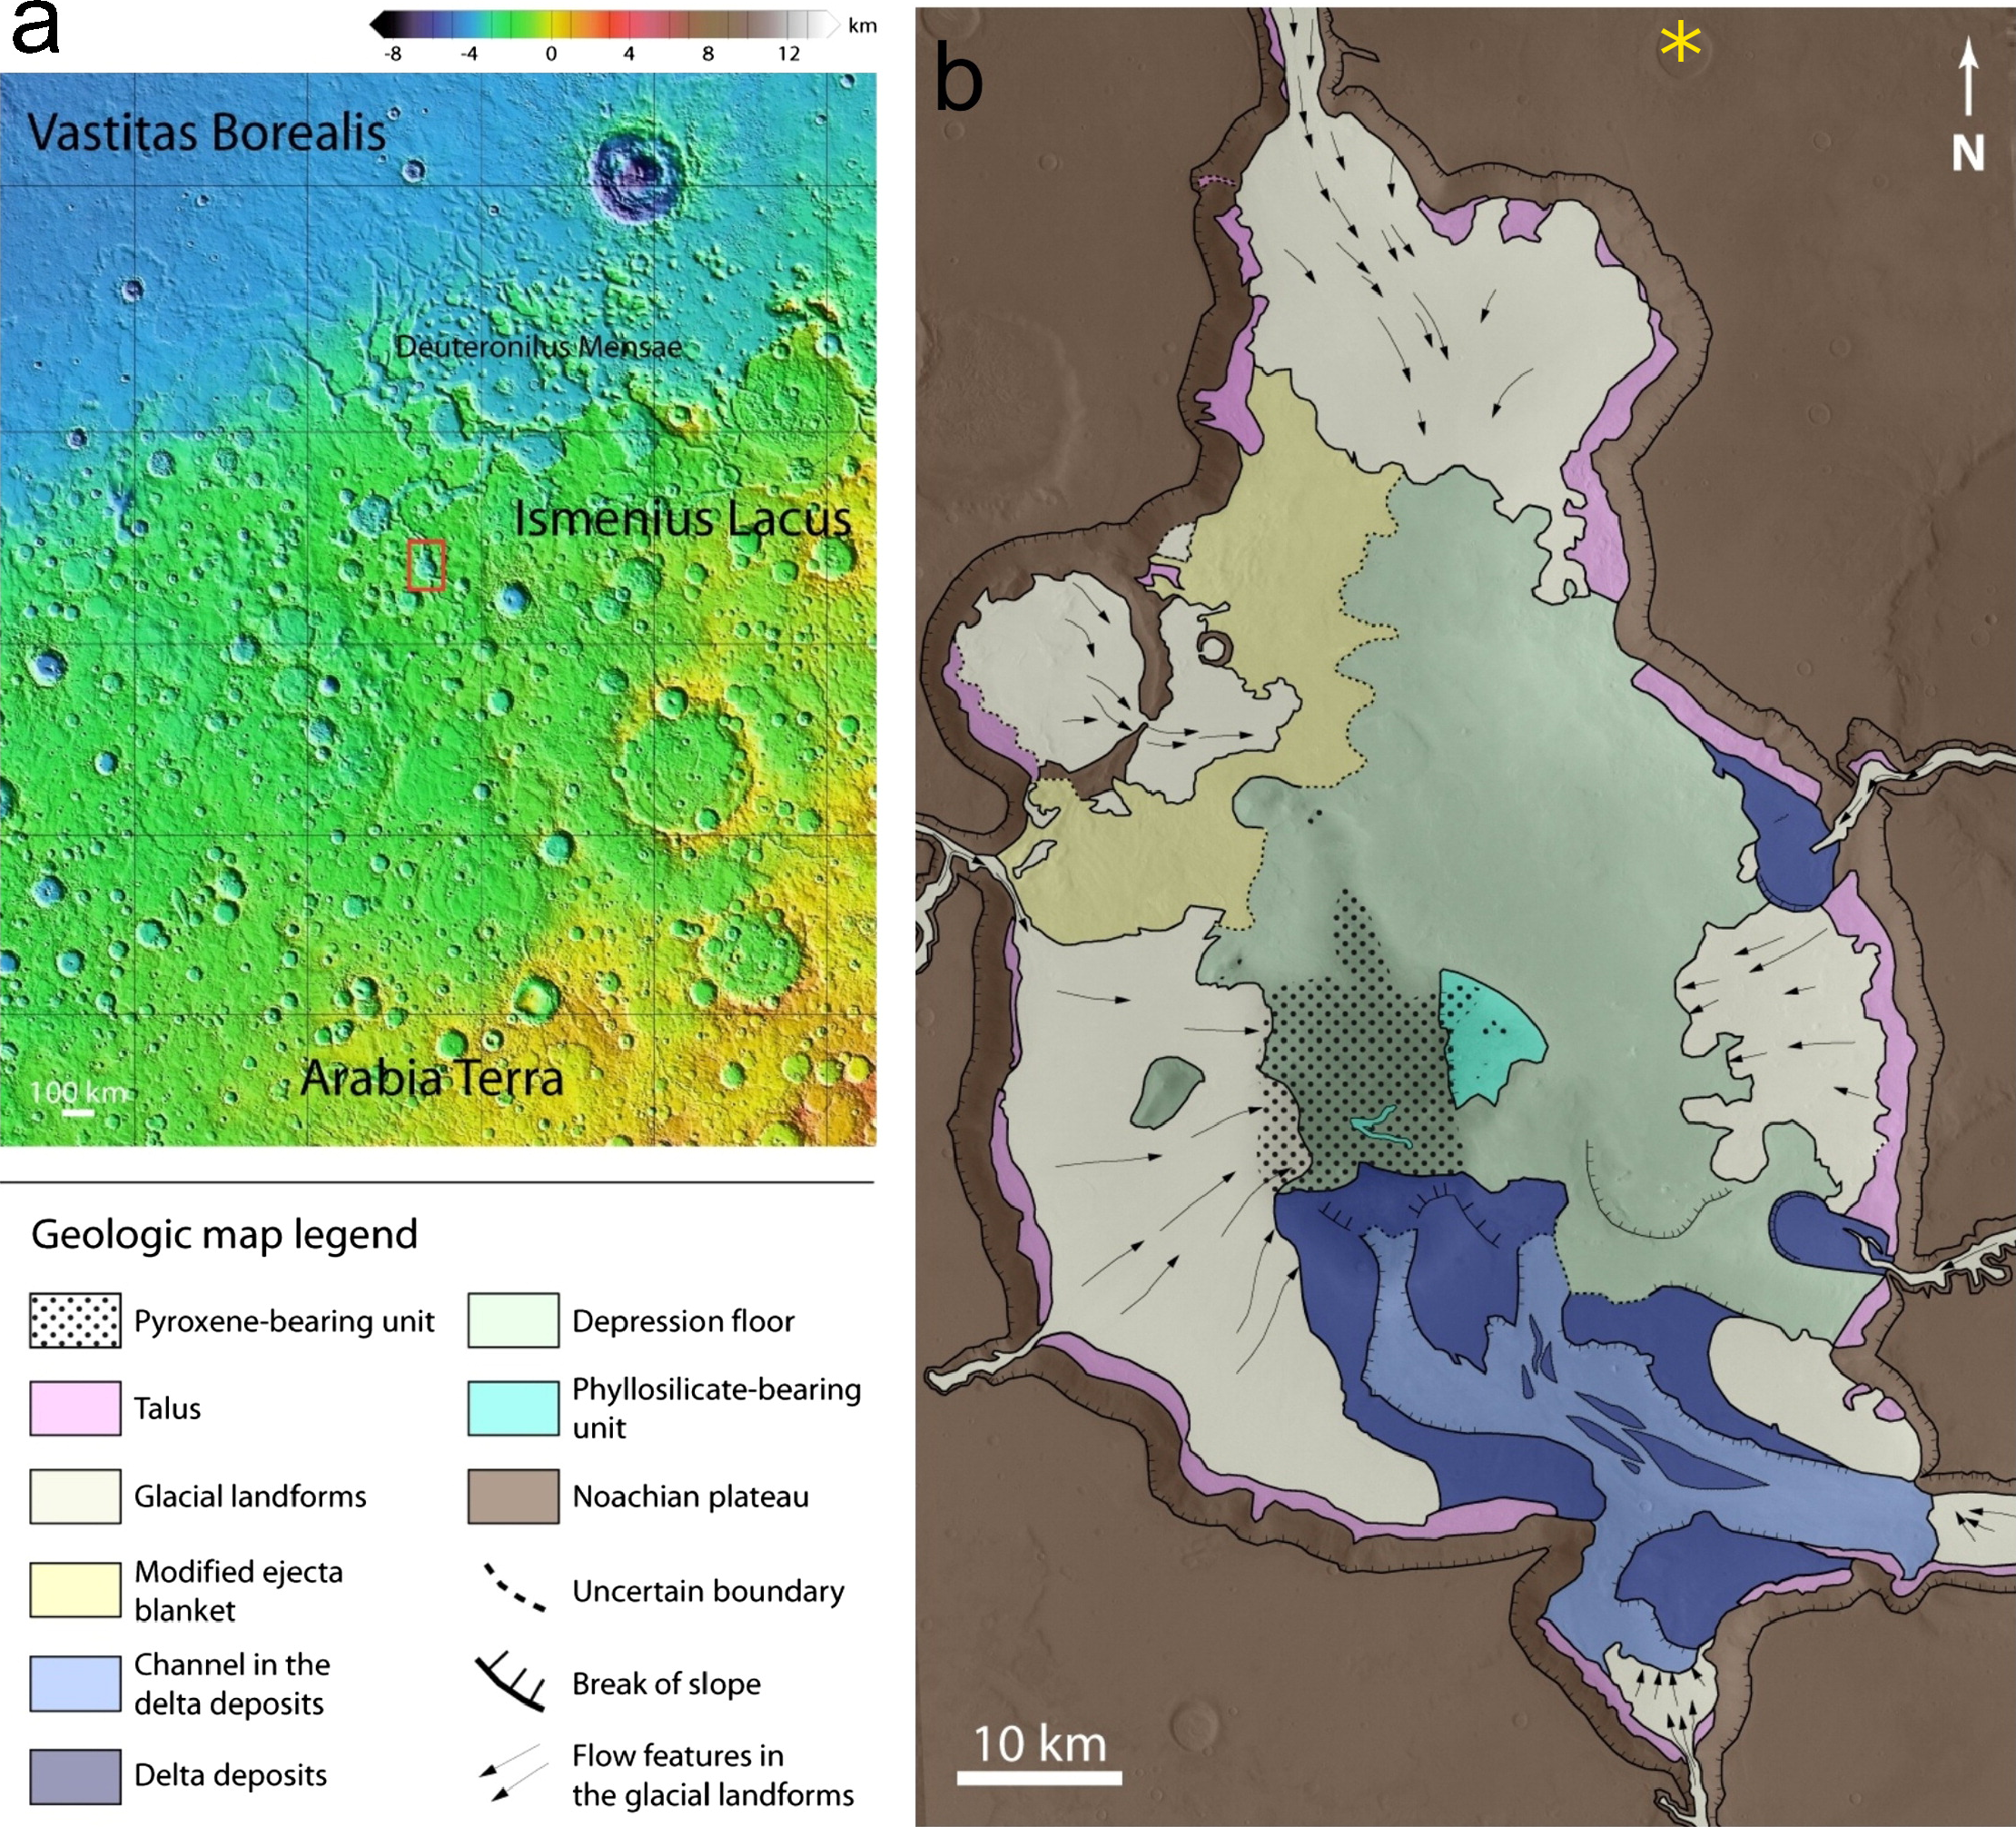
\includegraphics[width=0.6\linewidth]{sections/mars-solar-energy/mission-sites/images/ismenius-cavus.png}\\
  \caption[Geologic context of Ismenius Cavus mission site area]
          {Geologic context of Ismenius Cavus mission site area, taken from \citeother{Dehouck2010}. Location shown on a \ac{MOLA} reference map (a) and a geologic map of Ismenius Cavus (b). The yellow asterisk indicates the \ac{HiRISE} \ac{DTM} location which was used for mission scenario simulation.}
  \label{fig:mission-site-ismenius-cavus}
\end{figure}

% https://www.uahirise.org/dtm/dtm.php?ID=ESP_052945_2150

Supported science of interest are taken from \citeother{Dehouck2015}:
\begin{enumerate}[label=\textcolor{BulletBlue}{(\alph*)}]
    \item Potential for past habitability.
    \item Potential for organic matter with surface exposure.
    \item Noachian/Hesperian rocks with trapped atmospheric gases.
    \item High likelohood of surface-atmosphere exchange.
    \item Amazonian subsurface or high-latitude ice or sediment.
    \item Range of Martian geologic time; datable surfaces.
    \item Evidence of aqueous processes.
    \item Potential for interpreting relative ages.
    \item Near-surface ice, glacial or permafrost.
    \item Noachian or pre-Noachian bedrock units.
    \item Diversity of aeolian sediments and/or landforms.
\end{enumerate}

Supported resources of interest are also presented in \citeother{Dehouck2015} with clay minerals and water ice being two main resources for water. Furthermore, there is a potential for metal/silicon. These resources are located no more than \SI{3}{\meter} below the surface. Mobile material resources for construction purposes also exist.

\refFig{fig:sub:ismenius-cavus-dtm} shows a section of the \ac{DTM} which was loaded on the rover's mission simulation plaform. It features an exit breach in a well-preserved crater. The topography of the area is shown in \refFig{fig:sub:western-iani-chaos-dtm-altimetry}.
\vspace{0.5cm}

\begin{figure}[h]
\captionsetup[subfigure]{justification=centering}
\vspace{-2ex}
	\centering
    %% setup sizes
    \setlength{\subfigureWidth}{0.50\textwidth}
    \setlength{\graphicsHeight}{70mm}
    %% kill hyper-link highlighting
    \hypersetup{hidelinks=true}%
    %% the figures
    \begin{subfigure}[t]{\subfigureWidth}
        \centering
        \includegraphics[height=\graphicsHeight]{sections/mars-solar-energy/mission-sites/images/ismenius-cavus-dtm.png}
        \subcaption{\ac{DTM}}
        \label{fig:sub:ismenius-cavus-dtm}
    \end{subfigure}\hfill
    \begin{subfigure}[t]{\subfigureWidth}
        \centering
        \includegraphics[height=\graphicsHeight]{sections/mars-solar-energy/mission-sites/images/ismenius-cavus-dtm-altimetry.png}
  		\subcaption{Topography}
		\label{fig:sub:ismenius-cavus-dtm-altimetry}
	\end{subfigure}\\[0.8ex]
    \caption[Ismenius Cavus HiRISE digital terrain model]
            {Ismenius Cavus \ac{HiRISE} \ac{DTM}, taken from \citeother{AreoBrowser}. Image: \ac{NASA}/\ac{JPL}/University of Arizona.}
    \label{fig:ismenius-cavus}
\vspace{-2ex}
\end{figure}

\subsection{Daily Insolation}
Worst and best case daily insolations presented in this section are considered when sizing the rover's \ac{SA}. Optical depth is typically around $\tau = 0.4$ on clear days \citemarsenv{Smith2019} and $1 \leq \tau \leq 1.5$ during local dust storms \citemarsenv{Lemmon2015}. Daily insolations $\tau > 1.5$ were only considered for global dust storm season ($\SI{180}{\degree} < L_{s} < \SI{360}{\degree}$). Year long daily insolations for $\tau = 0.4$ at both sites are shown in \refFig{fig:plot:solar-insolations-for-different-beta} where the selected $\beta$ inclination angles are combined with their optimal $\gamma_c$ orientation angles. Descriptions of these angles are found in Appendix \ref{sec:Appendix:OptimalAngles}.

\begin{figure}[h]
\captionsetup[subfigure]{justification=centering}
\vspace{-2ex}
\centering
    %% setup sizes
    \setlength{\subfigureWidth}{0.50\textwidth}
    \setlength{\graphicsHeight}{60mm}
    %% kill hyper-link highlighting
    \hypersetup{hidelinks=true}%
    %% the figures
    \begin{subfigure}[t]{\subfigureWidth}
        \centering
            \includegraphics[height=\graphicsHeight]{sections/mars-solar-energy/mission-sites/plots/iani-chaos-solar-insolations-for-different-beta-inclinations.png}
            \subcaption{Iani Chaos.}
            \label{fig:plot:sub:solar-insolations-for-different-beta-iani-chaos}
    \end{subfigure}\hfill
    \begin{subfigure}[t]{\subfigureWidth}
        \centering
            \includegraphics[height=\graphicsHeight]{sections/mars-solar-energy/mission-sites/plots/ismenius-cavus-solar-insolations-for-different-beta-inclinations.png}
            \subcaption{Ismenius Cavus.}
            \label{fig:plot:sub:solar-insolations-for-different-beta-ismenius-cavus}
    \end{subfigure}\\[0.8ex]
    \caption[Daily insolations at mission sites]
    {Daily insolations at mission sites for different combinations of surface inclination and orientation angles.}
    \label{fig:plot:solar-insolations-for-different-beta}
\vspace{-2ex}
\end{figure}

Large values of $\beta$ are typically preferred in terms of resulting insolation. However, constraints imposed on the rover's active suspension system imposes a limit on the attainable inclination. As such, the optimal $\beta$ angle from which maximum insolation can be achieved, henceforth referred to as $\beta_{opt}$, may not be attainable. In such cases, the best possible $\beta$ angle is targetted, hereinafter referred to as $\beta_{best}$. Body pitch commands of up to \SI{10}{\degree} are experimentally evaluated during steep slope climbing in \citeother{Cordes2018}. Modeling higher pitch angles resulted in poor wheel-ground contact angle, as shown in \refFig{fig:postures-sa-beta}. This is due to the wheel-steering axis having the same tilt as the rover's body. The rover's attainable tilt is thus restricted to a maximum of \SI{10}{\degree}.

\begin{figure}[h]
\captionsetup[subfigure]{justification=centering}
%\vspace{-2ex}
	\centering
    %% setup sizes
    \setlength{\subfigureWidth}{0.50\textwidth}
    \setlength{\graphicsHeight}{50mm}
    %% kill hyper-link highlighting
    \hypersetup{hidelinks=true}%
    %% the figures
    \begin{subfigure}[t]{\subfigureWidth}
        \centering
        \includegraphics[height=\graphicsHeight]{sections/mars-solar-energy/mission-sites/images/sherpatt-render-surface-beta-13-deg.png}
        \subcaption{$\beta = \SI{13}{\degree}$}
        \label{fig:sub:postures-sa-beta-13-degree}
    \end{subfigure}\hfill
    \begin{subfigure}[t]{\subfigureWidth}
        \centering
        \includegraphics[height=\graphicsHeight]{sections/mars-solar-energy/mission-sites/images/sherpatt-render-surface-beta-22-deg.png}
  		\subcaption{$\beta = \SI{22}{\degree}$}
		\label{fig:sub:postures-sa-beta-22-degree}
	\end{subfigure}\\[0.8ex]
    \caption[SherpaTT body pitch \SI{13}{\degree} and \SI{22}{\degree}]
            {SherpaTT body pitch \SI{13}{\degree} and \SI{22}{\degree}.}
    \label{fig:postures-sa-beta}
\vspace{-2ex}
\end{figure}

\vspace{0.5cm}

Daily insolations on horizontal and inclined surfaces with $\beta_{best}=\pm\SI{10}{\degree}$\footnote{$\beta$ is positive in the northern hemisphere and negative in the southern hemisphere.} are presented in \refTab{tab:insolation-iani-chaos-clear-and-dusty-days} and \refTab{tab:insolation-iani-chaos-global-storm-days} for Iani Chaos and \refTab{tab:insolation-ismenius-cavus-clear-and-dusty-days} and \refTab{tab:insolation-ismenius-cavus-global-storm-days} for Ismenius Cavus. Gains obtained in daily insolation with an inclined surface are more pronounced for sites further away from the equator. For a typical optical depth of $\tau = 0.4$, the average daily insolation gain on the inclined surface is approximately \SI{7}{\percent} at Iani Chaos and \SI{9}{\percent} at Ismenius Cavus.
Due to the mostly diffuse composition of solar irradiance at higher optical depths, inclined surfaces become irrelevent during global dust storms. For $\tau \geq 2$, gains in daily insolation become negligeable at both mission sites.

\begin{table}[h]
\footnotesize
\centering
\caption[Worst and best case daily insolations for clear to dusty days at Iani Chaos]
{Worst and best case daily insolations for clear to dusty days at Iani Chaos. Daily insolation on an inclined surface $H_{\beta}$ is obtained with $\beta = \beta_{best} = \SI{-10}{\degree}$ and $\gamma_{c}$ set to optimal orientation angle.}
\label{tab:insolation-iani-chaos-clear-and-dusty-days}
\begin{tabular}{c|c|c|c|c|c|c|c|c|}
\cline{2-9}
\multicolumn{1}{l|}{} & \multicolumn{4}{c|}{\textbf{Worst Case}} & \multicolumn{4}{c|}{\textbf{Best Case}} \\ \hline
\multicolumn{1}{|c|}{$\tau$} & $L_{s}$ & $H_{h}$ & $H_{\beta}$ & $\%\:gain$ & $L_{s}$ & $H_{h}$ & $H_{\beta}$ & $\%\:gain$ \\ \hline
\multicolumn{1}{|c|}{\textbf{0.1}} & 80 & 3232 & 3721 & 15.13 & 221 & 5076 & 5695 & 12.19 \\ \hline
\multicolumn{1}{|c|}{\textbf{0.4}} & 81 & 2909 & 3166 & 8.85 & 218 & 4613 & 4933 & 6.93 \\ \hline
\multicolumn{1}{|c|}{\textbf{0.5}} & 81 & 2812 & 3025 & 7.58 & 218 & 4473 & 4736 & 5.89 \\ \hline
\multicolumn{1}{|c|}{\textbf{1.0}} & 82 & 2391 & 2479 & 3.67 & 214 & 3855 & 3959 & 2.69 \\ \hline
\multicolumn{1}{|c|}{\textbf{1.5}} & 82 & 2087 & 2125 & 1.81 & 213 & 3403 & 3444 & 1.19 \\ \hline
\end{tabular}
\end{table}


\vspace{0.5cm}

\begin{table}[h]
\footnotesize
\centering
\caption[Worst and best case daily insolations for global storm days at Iani Chaos]
{Worst and best case daily insolations for clear to global storm days at Iani Chaos. Daily insolation on an inclined surface $H_{\beta}$ is obtained with $\beta = \beta_{best} = \SI{-10}{\degree}$ and $\gamma_{c}$ set to optimal orientation angle.}
\label{tab:insolation-iani-chaos-global-storm-days}
\begin{tabular}{c|c|c|c|c|c|c|c|c|}
\cline{2-9}
\multicolumn{1}{l|}{} & \multicolumn{4}{c|}{\textbf{Worst Case}} & \multicolumn{4}{c|}{\textbf{Best Case}} \\ \hline
\multicolumn{1}{|c|}{$\tau$} & $L_{s}$ & $H_{h}$ & $H_{\beta}$ & $\%\:gain$ & $L_{s}$ & $H_{h}$ & $H_{\beta}$ & $\%\:gain$ \\ \hline
\multicolumn{1}{|c|}{\textbf{2.0}} & 360 & 2516 & 2519 & 0.10 & 212 & 3053 & 3066 & 0.42 \\ \hline
\multicolumn{1}{|c|}{\textbf{2.5}} & 360 & 2247 & 2243 & -0.18 & 211 & 2724 & 2723 & -0.02 \\ \hline
\multicolumn{1}{|c|}{\textbf{3.0}} & 360 & 1991 & 1985 & -0.32 & 210 & 2412 & 2406 & -0.27 \\ \hline
\multicolumn{1}{|c|}{\textbf{3.5}} & 360 & 1771 & 1763 & -0.45 & 210 & 2142 & 2134 & -0.37 \\ \hline
\multicolumn{1}{|c|}{\textbf{4.0}} & 360 & 1579 & 1572 & -0.44 & 209 & 1910 & 1901 & -0.47 \\ \hline
\multicolumn{1}{|c|}{\textbf{4.5}} & 360 & 1414 & 1406 & -0.54 & 209 & 1709 & 1700 & -0.54 \\ \hline
\multicolumn{1}{|c|}{\textbf{5.0}} & 360 & 1268 & 1261 & -0.58 & 209 & 1533 & 1523 & -0.62 \\ \hline
\end{tabular}
\end{table}


\vspace{0.5cm}

\begin{table}[h]
\footnotesize
\centering
\caption[Worst and best case daily insolations for clear to dusty days at Ismenius Cavus]
{Worst and best case daily insolations for clear to dusty days at Ismenius Cavus. Daily insolation on an inclined surface $H_{\beta}$ is obtained with $\beta = \beta_{best} = \SI{10}{\degree}$ and $\gamma_{c}$ set to optimal orientation angle.}
\label{tab:insolation-ismenius-cavus-clear-and-dusty-days}
\begin{tabular}{c|c|c|c|c|c|c|c|c|}
\cline{2-9}
\multicolumn{1}{l|}{} & \multicolumn{4}{c|}{\textbf{Worst Case}} & \multicolumn{4}{c|}{\textbf{Best Case}} \\ \hline
\multicolumn{1}{|c|}{$\tau$} & $L_{s}$ & $H_{h}$ & $H_{\beta}$ & $\%\:gain$ & $L_{s}$ & $H_{h}$ & $H_{\beta}$ & $\%\:gain$ \\ \hline
\multicolumn{1}{|c|}{\textbf{0.1}} & 274 & 2102 & 2762 & 31.42 & 127 & 4421 & 4925 & 11.40 \\ \hline
\multicolumn{1}{|c|}{\textbf{0.4}} & 273 & 1752 & 2030 & 15.85 & 125 & 4028 & 4289 & 6.49 \\ \hline
\multicolumn{1}{|c|}{\textbf{0.5}} & 273 & 1655 & 1869 & 12.93 & 124 & 3908 & 4122 & 5.48 \\ \hline
\multicolumn{1}{|c|}{\textbf{1.0}} & 273 & 1284 & 1345 & 4.75 & 121 & 3378 & 3461 & 2.44 \\ \hline
\multicolumn{1}{|c|}{\textbf{1.5}} & 273 & 1045 & 1061 & 1.57 & 120 & 2945 & 2973 & 0.96 \\ \hline
\end{tabular}
\end{table}


\vspace{0.5cm}

\begin{table}[h]
\footnotesize
\centering
\caption[Worst- and best-case daily insolations for global storm days at Ismenius Cavus]
{Worst- and best-case daily insolations for clear to global storm days at Ismenius Cavus. Daily insolation on an inclined surface $H_{\beta}$ is obtained with $\beta = \beta_{best} = \SI{10}{\degree}$ and $\gamma_{c}$ set to optimal orientation angle.}
\label{tab:insolation-ismenius-cavus-global-storm-days}
\begin{tabular}{c|c|c|c|c|c|c|c|c|}
\cline{2-9}
\multicolumn{1}{l|}{} & \multicolumn{4}{c|}{\textbf{Worst Case}} & \multicolumn{4}{c|}{\textbf{Best Case}} \\ \hline
\multicolumn{1}{|c|}{$\tau$} & $L_{s}$ & $H_{h}$ & $H_{\beta}$ & $\%\:gain$ & $L_{s}$ & $H_{h}$ & $H_{\beta}$ & $\%\:gain$ \\ \hline
\multicolumn{1}{|c|}{\textbf{2.0}} & 273 & 901 & 904 & 0.30 & 180 & 2155 & 2155 & 0.00 \\ \hline
\multicolumn{1}{|c|}{\textbf{2.5}} & 273 & 783 & 782 & -0.17 & 180 & 1899 & 1891 & -0.43 \\ \hline
\multicolumn{1}{|c|}{\textbf{3.0}} & 273 & 677 & 675 & -028 & 180 & 1664 & 1654 & -0.61 \\ \hline
\multicolumn{1}{|c|}{\textbf{3.5}} & 273 & 589 & 586 & -0.48 & 180 & 1467 & 1456 & -0.75 \\ \hline
\multicolumn{1}{|c|}{\textbf{4.0}} & 273 & 516 & 514 & -0.35 & 180 & 1300 & 1290 & -0.80 \\ \hline
\multicolumn{1}{|c|}{\textbf{4.5}} & 273 & 462 & 460 & -0.37 & 180 & 1158 & 1149 & -0.80 \\ \hline
\multicolumn{1}{|c|}{\textbf{5.0}} & 273 & 424 & 422 & -0.54 & 180 & 1038 & 1028 & -0.98 \\ \hline
\end{tabular}
\end{table}


The worst-case slope traverse is an on inclined surface facing opposite the equator. This can be mitigated by using the rover's suspension system to compensate with a tilt in the opposite direction, as illustrated in \refFig{fig:sub:rover-on-slope-beta} where $B$ denotes the slope surface inclination angle and $\beta$ the \ac{SA} surface inclination angle. This scenario will be further explored in \refSec{sec:Design:Simulation}. By way of example, at Ismenius Cavus for $\tau = 0.4$ and $L_{s}=\SI{270}{\degree}$, descending a \SI{30}{\degree} slope bearing North results in a daily insolation of \SI{319}{Whm^{-2}}. This can be increased to \SI{767}{Whm^{-2}} by decreasing $\beta$ from \SI{30}{\degree} to \SI{25}{\degree} after tilting the rover southwards by \SI{5}{\degree} so that $\beta < B$ with $\beta = \SI{25}{\degree}$. A \SI{10}{\degree} tilt would increase the daily insolation to \SI{1046}{Whm^{-2}} with $\beta = \SI{20}{\degree}$.


\begin{figure}[h]
\captionsetup[subfigure]{justification=centering}
%\vspace{-2ex}
	\centering
    %% setup sizes
    \setlength{\subfigureWidth}{0.50\textwidth}
    \setlength{\graphicsHeight}{40mm}
    %% kill hyper-link highlighting
    \hypersetup{hidelinks=true}%
    %% the figures
    \begin{subfigure}[t]{\subfigureWidth}
        \centering
        \includegraphics[height=\graphicsHeight]{sections/mars-solar-energy/mission-sites/images/stick-rover-beta-large.png}
        \subcaption{$\beta = B$}
        \label{fig:sub:rover-on-slope-beta-large}
    \end{subfigure}\hfill
    \begin{subfigure}[t]{\subfigureWidth}
        \centering
        \includegraphics[height=\graphicsHeight]{sections/mars-solar-energy/mission-sites/images/stick-rover-beta-small.png}
  		\subcaption{$\beta < B$}
		\label{fig:sub:rover-on-slope-beta-small}
	\end{subfigure}\\[0.8ex]
    \caption[Slope compensation with active suspension system]
            {Slope compensation with active suspension system to reduce the \ac{SA} surface inclination angle. Slope inclination angle $B = \SI{30}{\degree}$. In (a), $\beta = B = \SI{30}{\degree}$. In (b), the rover is tilted  \SI{10}{\degree} in the opposite direction of the slope so that $\beta = \SI{20}{\degree}$.}
    \label{fig:sub:rover-on-slope-beta}
%\vspace{-2ex}
\end{figure}


\subsection{Summary}
Available solar insolation have been constrained by identifying two mission sites based on set of selection criteria. The need to navigate complex topographic morphologies at these sites also introduces considerations for \ac{SA} inclination strategies. Large differences in planetary latitudes between both sites ensures that several environmental variations are considered.


\section{Summary and Conclusion}
\label{sec:MarsSolarEnergy:SummaryAndConclusion}
Understanding the dynamics of the Martian solar radiation environment is a crucial prequisite to  conceptualizing feasible mission scenarios. In this chapter, the potenial solar power and energy outputs were constrainted with mission site selections. Two locations were identified so that rover task planning and \ac{SA} sizing processes may appreciate a richer set of consequences tied to a wider range of environmental variables.

%%%%%%%%%%%%%%%%%%%%%%%%%%%%%%%%%%%%%%%%%%%%%%%%%%%%%%%


%%%%%%%%%%%%%%%%%%%%%%%%%%%%%%%%%%%%%%%%%%%%%%%%%%%%%%%
\chapter{Power System Design}
\label{sec:PowerSystemDesign}
\shinyChapterQuote{For the human makers of things, the incompletenesses and inconsistencies of our ideas become clear only during implementation.}
  {Frederick P. Brooks Jr} %The Mythical Man-Month: Essays on Software Engineering
This chapter elaborates on the power budget and requirements leading to the proposed solar array design. Reference Sols and their rover modes are defined in \refSec{sec:Design:ReferenceSols} so that mission scenario power budgets may be formalized in \refSec{sec:Design:PowerBudget}. Particular attention is put on analyzing field trial data from which propulsion power draw requirements are extracted. \refSec{sec:Design:RequirementsAndDesignDrivers} consolidates assumptions, requirements, conwtraints, and design drivers that will guide the proposed design of the rover's \ac{PV} system. Solar array sizing and configurations as well as necessary rover body redesign are presented in \refSec{sec:Design:SolarArray}. A rudimentary simulation environment for solar power management is introduced in \refSec{sec:Design:Simulation} as a potential for future work before summarizing and concluding the chapter in \refSec{sec:Design:SummaryAndConclusion}.

\section{Reference Sols}
\label{sec:Design:ReferenceSols}
Baseline content for this section were taken from \citeother{CDF2014} and constrained to the scope of this thesis. Adjustements were made in relation to the mission sites described in the previous chapter as well as with the rover's capabilities with respect to its active suspension system. Rover modes were identified and then sequenced into high-level reference Sols for mission planning. Defining rover modes and reference Sols served as a prerequisite to formalizing power budgets by assignment each rover modes with their power draw and minimal operational duration.

%The chapter is structured as follows: Section \ref{sec:ReferenceSols:RoverModes} provides general definitions of rover modes. The identified rover modes are sequenced into reference Sols in Section \ref{sec:ReferenceSols:ReferenceSols}. The chapter is then summarized in Section \ref{sec:PowerBudget:SummaryAndConclusion}.

\subsection{Rover Modes}
\label{sec:ReferenceSols:RoverModes}
Not all modes defined in \citeother{CDF2014} were included in this section, however; they may become of interest in future design iterations. The omitted modes are \textit{Launch}, \textit{\ac{EDL}}, \textit{Deployment}, \textit{Science Stop - Long},  and \textit{Safe} modes. The rover modes considered in this thesis are as follow:

\begin{itemize}
    \item \textbf{Traverse - Flat:} Pre-planned flat surface traverses to target destinations.
    \item \textbf{Traverse - Upslope:} Pre-planned upslope surface traverses to target destinations.
    \item \textbf{Science Stop - Short:} Short science activities in between traverses.
    \item \textbf{\ac{DTE} Communication:} Pre-planned communication sessions.
    \item \textbf{Idle - Day:} All day dedicated to charging batteries.
    \item \textbf{Idle - Night:} Minimal battery usage during night.
    \item \textbf{Hibernation:} Survival mode during dust storms ($\tau \geq 2$).
    \item \textbf{Optimal Pose:} Repositioning the rover along its principal yaw, pitch, and roll axes to maximized next Sol solar array power generation.
\end{itemize}
%\ac{DTE} Communication operations are encapsulated as their own mode whereas \ac{UHF} Communications are mode activities conducted during \textit{Traverse}, \textit{Science Stop}, and \textit{Idle} modes.

%Communication operations and their schedules were also taken from \citeother{CDF2014}:
%\begin{itemize}
%    \item Uplink of sol plan either early in the morning (\SI{30}{\minute} \ac{DTE} or \SI{7}{\minute} \ac{UHF}) or during the night (\SI{7}{\minute} \ac{UHF}).
%    \item Downlink of high priority data required for planning of the next sol either in the afternoon (\SI{5}{\minute} \ac{DTE}) or during the night (\SI{7}{\minute} \ac{UHF}).
%\end{itemize}

The \textit{Optimal Pose} mode was not taken from \citeother{CDF2014}. It was created for the purpose of this study so that the rover may use its active suspension system as a solar tracking mechanism to maximize \ac{SA} power generation. For the sake of simplicity, a constraint was applied to the pitch and roll axes which mutually excluded them from both being actuated. Thus, during the \textit{Optimal Pose} mode, only yaw-pitch or yaw-roll rotation combinations are allowed. The inclination angle resulting from a pith or roll rotations is the $\beta$ angle. The orientation angle with respect to the direction of the equator which resulting from a yaw rotation is the surface azimuth angle $\gamma_{c}$. These angles were introduced in Section \ref{sec:MartianEnvironment:SolarRadiation:InclinedSurface}.

Rover subsystems as well as their states during the rover modes were taken from \citeother{CDF2014} and are shown in Table \ref{tab:rover-modes}.

 %Some mode durations were adjusted from those presented in \citeother{CDF2014} in response to power budgeting constraints pertaining to the scope of this research.

\begin{table}[h]
\footnotesize
\centering
\caption[Rover modes]
    {Rover modes. DT/NT - Daytime/Night-time; BC - Battery Charging; P - Propulsion; N - Navigation; C - Communication; S - Science; H - Heaters. Duration is per Sol.}
\label{tab:rover-modes}
\begin{tabular}{|l|c|c|c|c|c|c|c|l|}
\hline
\textbf{Name} & \textbf{DT/NT} & \textbf{BC} & \textbf{P} & \textbf{N} & \textbf{C} & \textbf{S} & \textbf{H} & \textbf{Duration} \\ \hline
Traverse - Flat & DT & OFF & ON & ON & ON & OFF & OFF & Variable \\ \hline
Traverse - Upslope & DT & OFF & ON & ON & ON & OFF & OFF & Variable \\ \hline
Science Stop - Short & DT & ON & OFF & OFF & ON & ON & OFF & 60 min \\ \hline
\ac{DTE} Commnunication & DT & OFF & OFF & OFF & ON & OFF & OFF & 35 min \\ \hline
Idle - Day & DT & ON & OFF & OFF & ON & OFF & OFF & All day \\ \hline
Idle - Night & NT & OFF & OFF & OFF & ON & OFF & ON & All night \\ \hline
Hibernation & DT/NT & OFF & OFF & OFF & OFF & OFF & ON & All day/night \\ \hline
Optimal Pose & DT & ON & \multicolumn{1}{l|}{ON} & \multicolumn{1}{l|}{OFF} & \multicolumn{1}{l|}{ON} & \multicolumn{1}{l|}{OFF} & \multicolumn{1}{l|}{OFF} & 10 min \\ \hline
\end{tabular}
\end{table}




\subsection{Reference Sols}
\label{sec:ReferenceSols:ReferenceSols}
Flat and upslope traverses are the worst-case modes in terms of energy consumption at two different topographies. Hibernation must be constrained with respect to battery depletion in order to appreciate the rover's survivabilty during a dust storm. As such, only the \textit{Flat Traverse}, \textit{Upslope Traverse}, and \textit{Hibernation} reference Sols required analysis.


\subsubsection{Traverse Sol}
\label{sec:ReferenceSols:TraverseSol}
A \textit{Traverse Sol} allows the rover to reach a pre-planned target destination. Flat and upslope traverses have identical mode sequences, shown in Table \ref{tab:mission-scenario-traverse-sol}, only differing in the duration of their respective \textit{Traverse} modes. This distinction relates to propulsion power draw differences that are presented in Chapter \ref{sec:PowerBudget}.

\begin{table}[h]
\footnotesize
\centering
\caption{Reference Sol for flat or upslope traverse.}
\label{tab:mission-scenario-traverse-sol}
\begin{tabular}{|l|l|}
\hline
\textbf{Mode} & \textbf{Description} \\ \hline
\textbf{Idle - Day} & \begin{tabular}[c]{@{}l@{}}Pre-Heating.\\ UHF Communication.\\ Battery Charging.\end{tabular} \\ \hline
\textbf{DTE Communication} & \begin{tabular}[c]{@{}l@{}}Downlink.\\ Uplink.\end{tabular} \\ \hline
\textbf{Traverse - Flat or Upslope} & Propulsion to target destination. \\ \hline
\textbf{Science Stop - Short} & Science operations. \\ \hline
\textbf{Optimal Pose} & Maximize SA power generation for next Sol. \\ \hline
\textbf{Idle - Night} & \begin{tabular}[c]{@{}l@{}}UHF Communication.\\ Thermal Regulation.\end{tabular} \\ \hline
\end{tabular}
\end{table}


A Traverse Sol begins with the \textit{Idle - Day} mode, which is mostly dedicated to recharging the rover's batteries. On the previous Sol, the \ac{SA} was tilted and oriented into an optimal configuration with respect to the current SoL's sun path in order to maximize power generation. The \textit{\ac{DTE} Communication} mode follows after which the received traversing commands are processed during the \textit{Traverse} mode. A short time slot is alotted to science operations during the \textit{Science Stop - Short} mode so that multiple traverse Sols do not result in lack of scientific return, particularly for long multi-Sol traverse campaigns. The rover then assumes an optimal power generation pose during the \textit{Optimal Pose} mode to ensure maximum \ac{SA} power generation on the next Sol. Finally, the \textit{Idle - Night} mode is engaged during which the rover's survival is ensured with heaters that thermally regulate all critical systems.

The mechanical feasibility of achieving $\beta_{opt}$ or $\beta_{best}$ does not imply operational feasibility with respect to other subsystems. For instance, pitching the rover may hinder communication \ac{LOS} or produce thermal imbalances that would complicate heating the rover's critical systems. The implications are a systems engineering problem that is beyond the scope of this study. The assumption was made that all rover subsystems are designed to functional nominally for $\beta_{opt}$ and $\beta_{best}$.

%\subsection{Science Sol}
%\label{sec:ReferenceSols:ScienceSol}
%The Science Sol maximizes science data collection. The mode sequence is shown in Table \ref{tab:mission-scenario-science-sol}. It only differs from the Traverse Sol with a \textit{Science Stop - Long} mode instead of a \textit{Traverse} mode.
%\input{sections/design/reference-sols/tables/mission-scenario-science-sol.tex}

%\clearpage
%\subsection{Battery Recharge Sol}
%\label{sec:ReferenceSols:BatteryRechargeSol}
%The Battery Recharge Sol dedicates an entire Martian day to recharging the rover's batteries. The sequence and duration of its modes are shown in Table \ref{tab:mission-scenario-science-sol}. Only thermal and communication operations are executed during this Sol so that power draws from the battery are minimized in order to prioritize attaining the target charge state. No rover repositioning is required to adjust the \ac{SA} $\beta$ angle as it will have already been set to $\beta_{optimal}$ or $\beta_{best}$ at the end of a previous Sol.

%\begin{table}[h]
\footnotesize
\centering
\caption[Battery Charging Sol mission scenario]
    {Battery Charging Sol mission scenario.}
\label{tab:mission-scenario-battery-charging-sol}
\begin{tabular}{l|l|c|c|}
\hline
\multicolumn{1}{|l|}{\multirow{2}{*}{\begin{tabular}[c]{@{}l@{}}\\\textbf{Mode}\\\end{tabular}}} & \multirow{2}{*}{\begin{tabular}[c]{@{}l@{}}\\\textbf{Description}\\\end{tabular}} & \multicolumn{2}{c|}{\textbf{Duration {[}min{]}}} \\ \cline{3-4}
\multicolumn{1}{|l|}{} &  & \multicolumn{1}{l|}{\begin{tabular}[c]{@{}c@{}}\textbf{Iani}\\\textbf{Chaos}\end{tabular}} & \multicolumn{1}{l|}{\begin{tabular}[c]{@{}c@{}}\textbf{Ismenius}\\\textbf{Cavus}\end{tabular}} \\ \hline
\multicolumn{1}{|l|}{\textbf{Idle - Day}} & \begin{tabular}[c]{@{}l@{}}Pre-Heating (2 hr).\\ UHF Communication (7 min).\\ Battery Charging.\end{tabular} & 88 & 88 \\ \hline
\multicolumn{1}{|l|}{\textbf{Idle - Night}} & \begin{tabular}[c]{@{}l@{}}UHF Communication (7 min).\\ Thermal Regulation.\end{tabular} & 88 & 88 \\ \hline
 & \multicolumn{1}{r|}{\textbf{Total Duration {[}min{]}}} & \textbf{999} & \textbf{999} \\ \cline{2-4}
\end{tabular}
\end{table}


\subsubsection{Hibernation Sol}
\label{sec:ReferenceSols:HibernationSol}
The Hibernation Sol is the rover's survival mode during a dust storm. In this setting the rover solely draws power from its battery hence only the heater and a timer are on in order to conserve energy.

\begin{table}[h]
\footnotesize
\centering
\caption{Reference Sol for hibernation.}
\label{tab:mission-scenario-hibernation-sol}
\begin{tabular}{|l|l|}
\hline
\textbf{Mode} & \textbf{Description} \\ \hline
\textbf{Hibernation - Day} & \begin{tabular}[c]{@{}l@{}}All day.\\ Battery draw kept to a minimum.\end{tabular} \\ \hline
\textbf{Hibernation - Night} & \begin{tabular}[c]{@{}l@{}}All night.\\ Battery draw kept to a minimum.\end{tabular} \\ \hline
\end{tabular}
\end{table}


\subsection{Summary}
\label{sec:ReferenceSols:SummaryAndConclusion}
The section presents selected rover's modes which were used to define reference Sols. Of particular interest is the \textit{Optimal Mode} mode which takes advantage of the rover's active suspect system to maximize power generation and battery charging during the \textit{Idle - Day} mode. Distinctions were made between two types of \textit{Traverse} modes with respect to flat or upslope terrain topography.

% Operation durations were established for each mode as a prerequesite to determining power budgets in the following chapter.


\section{Power Budget}
\label{sec:Design:PowerBudget}
This section details the power budget for the reference Sols used in mission planning. Propulsion power budgets for the rover's Traverse modes were determined from data collected during the SherpaTT field trials in Utah. Power budgets for other rover modes that make up the reference Sols were taken from \citeother{CDF2014}.

%The chapter is structured as follows: Propulsion power budget are presented in Section \ref{sec:PowerBudget:PropulsionPowerBudget} following an analysis of Mars analogue field test campaign data. Rover modes that were presented in the previous Chapter are complemented with power budgets in Section \ref{sec:PowerBudget:RoverModePowerBudget}. The chapter is then summarized in Section \ref{sec:PowerBudget:SummaryAndConclusion}.

\subsection{Propulsion Power}
\label{sec:PowerBudget:PropulsionPowerBudget}
SherpaTT's actively articulated suspension system consists of four wheeled-legs with a total of 20 motors. Each leg is equipped with three suspension motors and two drive motors. The suspension motors are responsible for Pan, \ac{IL}, and \ac{OL} revolute joint rotations whereas the drive motors are responsible for \ac{WS} and \ac{WD}. The distribution of these motors across each leg are shown in Figure \ref{fig:sherpatt-actively-articulated-suspension-system}. Propulsion power draw refers to the summation of suspension and drive motor power draws. These power draws have been studied in detail for SherpaTT during a Mars analogue field campaign in Utah \citeother{Cordes2018}.

\begin{figure}[h]
  \centering
  \hypersetup{linkcolor=captionTextColor}
  \includegraphics[width=0.6\linewidth]{sections/design/power-budget/images/sherpatt-actively-articulated-suspension-sytem.png}\\
  \caption[SherpaTT actively articulated suspension system]
          {SherpaTT actively articulated suspension system, taken from \citeother{Cordes2018}.}
  \label{fig:sherpatt-actively-articulated-suspension-system}
\end{figure}

Lack of motor optimisation as well as lower gravity and pressure on Mars permit the assumption that, given similar topology traversals, measured propulsion power draws are greater than those that would be observed on a Martian environment. This assumption is further supported when considering that SherpaTT's velocities during power draw measurements were much greater than what has been achieved on present and past Mars rover missions.

Available datasets from the Mars analogue field test campaign cover two flat surface runs and three steep upslope terrain runs. From the two upslope runs, the dataset with the worst-case maximum and mean propulsion power draw was used as the worst-case scenario. Hereafter, all mention of SherpaTT power draws will reference measurements included in these datasets. Measured power draws fluctuate due to slips, skids, noise, and other unknown imperfections. To ease readability, local minima, maxima, and media lines have been traced for all power plot figures.

\subsubsection{Flat Terrain Traverse}
\label{sec:PowerBudget:PropulsionPowerBudget:FlatTerrainTraverse}
Both \ac{MER} and \ac{MSL} rovers are each equipped with a total of 10 propulsion motors to drive their Rocker-Bogie passive suspension system: six to rotate the wheels and four to steer them \citeother{Novak2005} \citeother{Lakdawalla2018}. The \ac{MER} rovers needed approximately \SI{100}{\watt} to drive \citeother{MERRoverEnergy}. Equation \ref{eq:InitialPropulsionPowerEstimate} was used for to determine an initial SherpaTT propulsion power draw using a single \ac{MER} wheel power draw as an estimation unit:

\begin{align}
  \label{eq:InitialPropulsionPowerEstimate}
  P_{prop}^{sherpatt} &= \frac{P_{prop}^{mer}}{N_{wheels}^{mer}} \times N_{wheels}^{sherpatt} \times \left(1 +\frac{P_{susp}^{sherpatt}}{P_{prop}^{sherpatt}}\right) \\
           &= \frac{100}{6} \times 4 \times 1.17\\
           &= \SI{78}{\watt}
\end{align}


where $P_{prop}$ is the total propulsion power, $P_{susp}$ is the total suspension power, $N_{wheels}$ is the number of wheels, and $P_{susp}^{sherpatt} / P_{prop}^{sherpatt}$ is the suspension system's share of the total propulsion power. For the latter, a worst-case 17\% was taken from \citeother{Cordes2018} for data collected from a flat terrain outdoor setting.

The propulsion power draws measured for SherpaTT on flat surface runs are shown in Figure \ref{fig:plot:sherpatt-flat-terrain-power-draw}. These measurements are summarised in Table \ref{tab:sherpatt-flat-terrain-global-minimum-maximum-and-medium-power-draws}. To eliminate power draw fluctuations from the analysis, only local media values were considered. Local media were selected rather than the worst-case local maxima on the basis of the assumptions made in Section \ref{sec:PowerBudget:PropulsionPowerBudget}. For flat terrain traverses, a worst-case maximum power draw of \SI{74}{\watt} is observed in close accordance with the initial estimate obtained from Equation \ref{eq:InitialPropulsionPowerEstimate}.

\begin{figure}[h]
\captionsetup[subfigure]{justification=centering}
\vspace{-2ex}
	\centering
    %% setup sizes
    \setlength{\subfigureWidth}{0.50\textwidth}
    \setlength{\graphicsHeight}{80mm}
    %% kill hyper-link highlighting
    \hypersetup{hidelinks=true}%
    %% the figures
    \begin{subfigure}[t]{\subfigureWidth}
        \centering
        \includegraphics[height=\graphicsHeight]{sections/design/power-budget/plots/locomotion-power-draw-on-flat-terrain-1.png}
        \subcaption{Run \#1}
        \label{fig:plot:sub:sherpatt-flat-terrain-power-draw-1}
    \end{subfigure}\hfill
    \begin{subfigure}[t]{\subfigureWidth}
        \centering
        \includegraphics[height=\graphicsHeight]{sections/design/power-budget/plots/locomotion-power-draw-on-flat-terrain-2.png}
  		\subcaption{Run \#2}
		\label{fig:plot:sub:sherpatt-flat-terrain-power-draw-2}
	\end{subfigure}\\[0.8ex]
    \caption[Propulsion power draw for a flat terrain traverse during SherpaTT Mars analogue field tests in Utah]
            {Propulsion power draw for a flat terrain traverse during SherpaTT Mars analogue field tests in Utah.}
    \label{fig:plot:sherpatt-flat-terrain-power-draw}
\vspace{-2ex}
\end{figure}



\begin{table}[h]
\footnotesize
\centering
\caption[Global minimum, maximum, and medium of traced local minima, maxima, and media for SherpaTT flat terrain propulsion power draw lines]
    {Global minimum, maximum, and medium of traced local minima, maxima, and media for SherpaTT flat terrain propulsion power draw lines.}
\label{tab:sherpatt-flat-terrain-global-minimum-maximum-and-medium-power-draws}
\begin{tabular}{llccc}
\cline{3-5}
\multicolumn{2}{l|}{\multirow{2}{*}{}} & \multicolumn{3}{c|}{\textbf{Power Draw {[}W{]}}} \\ \cline{3-5}
\multicolumn{2}{l|}{} & \multicolumn{1}{c|}{\textbf{\begin{tabular}[c]{@{}c@{}}Global Minimum\end{tabular}}} & \multicolumn{1}{c|}{\textbf{\begin{tabular}[c]{@{}c@{}}Global Maximum\end{tabular}}} & \multicolumn{1}{c|}{\textbf{\begin{tabular}[c]{@{}c@{}}Global Media\end{tabular}}} \\ \hline
\multicolumn{1}{|c|}{\multirow{4}{*}{\textbf{Run \#1}}} & \multicolumn{1}{l|}{\textbf{Measured}} & \multicolumn{1}{c|}{27} & \multicolumn{1}{c|}{114} & \multicolumn{1}{c|}{60} \\ \cline{2-5}
\multicolumn{1}{|c|}{} & \multicolumn{1}{l|}{\textbf{Local Minima}} & \multicolumn{1}{c|}{27} & \multicolumn{1}{c|}{50} & \multicolumn{1}{c|}{38} \\ \cline{2-5}
\multicolumn{1}{|c|}{} & \multicolumn{1}{l|}{\textbf{Local Maxima}} & \multicolumn{1}{c|}{69} & \multicolumn{1}{c|}{114} & \multicolumn{1}{c|}{83} \\ \cline{2-5}
\multicolumn{1}{|c|}{} & \multicolumn{1}{l|}{\textbf{Local Media}} & \multicolumn{1}{c|}{52} & \multicolumn{1}{c|}{74} & \multicolumn{1}{c|}{61} \\ \hhline{|=|=|=|=|=|}
\multicolumn{1}{|l|}{\multirow{4}{*}{\textbf{Run \#2}}} & \multicolumn{1}{l|}{\textbf{Measured}} & \multicolumn{1}{c|}{17} & \multicolumn{1}{c|}{101} & \multicolumn{1}{c|}{51} \\ \cline{2-5}
\multicolumn{1}{|l|}{} & \multicolumn{1}{l|}{\textbf{Local Minima}} & \multicolumn{1}{c|}{17} & \multicolumn{1}{c|}{42} & \multicolumn{1}{c|}{30} \\ \cline{2-5}
\multicolumn{1}{|l|}{} & \multicolumn{1}{l|}{\textbf{Local Maxima}} & \multicolumn{1}{c|}{52} & \multicolumn{1}{c|}{101} & \multicolumn{1}{c|}{74} \\ \cline{2-5}
\multicolumn{1}{|l|}{} & \multicolumn{1}{l|}{\textbf{Local Media}} & \multicolumn{1}{c|}{40} & \multicolumn{1}{c|}{64} & \multicolumn{1}{c|}{52} \\ \hline
 &  & \multicolumn{1}{l}{} & \multicolumn{1}{l}{} & \multicolumn{1}{l}{} \\
 &  & \multicolumn{1}{l}{} & \multicolumn{1}{l}{} & \multicolumn{1}{l}{}
\end{tabular}
\end{table}


\pagebreak
\subsubsection{Upslope Terrain Traverse}
\label{sec:PowerBudget:PropulsionPowerBudget:UpslopeTerrainTraverse}
Propulsion power draws on a steep uplsope were measured along an approximately \SI{16}{\meter} track and are shown Figure \ref{fig:plot:sub:sherpatt-disaggregated-upslope-terrain-power-draw-locomotion}. An initial estimate of \SI{132}{\watt} was obtained using Equation \ref{eq:InitialPropulsionPowerEstimate} with a worst case 98\% suspension system's share of the total propulsion power taken from \citeother{Cordes2018} for data collected from a steep slope outdoor setting. The drive and suspension power draw components are shown in Figures \ref{fig:plot:sub:sherpatt-disaggregated-upslope-terrain-power-draw-drive} and \ref{fig:plot:sub:sherpatt-disaggregated-upslope-terrain-power-draw-suspension}, respectively.

\begin{figure}[h]
\captionsetup[subfigure]{justification=centering}
\vspace{-2ex}
	\centering
    %% setup sizes
    \setlength{\subfigureWidth}{0.32\textwidth}
    \setlength{\graphicsHeight}{50mm}
    %% kill hyper-link highlighting
    \hypersetup{hidelinks=true}%
    %% the figures
	\begin{subfigure}[t]{\subfigureWidth}
        \centering
        \includegraphics[height=\graphicsHeight]{sections/design/power-budget/plots/locomotion-power-draw-on-upslope-terrain.png}
  		\subcaption{Propulsion}
		\label{fig:plot:sub:sherpatt-disaggregated-upslope-terrain-power-draw-locomotion}
	\end{subfigure}\hfill
	\begin{subfigure}[t]{\subfigureWidth}
        \centering
        \includegraphics[height=\graphicsHeight]{sections/design/power-budget/plots/drive-power-draw-on-upslope-terrain.png}
  		\subcaption{Drive}
		\label{fig:plot:sub:sherpatt-disaggregated-upslope-terrain-power-draw-drive}
	\end{subfigure}\hfill
    \begin{subfigure}[t]{\subfigureWidth}
        \centering
        \includegraphics[height=\graphicsHeight]{sections/design/power-budget/plots/suspension-power-draw-on-upslope-terrain.png}
  		\subcaption{Suspension}
		\label{fig:plot:sub:sherpatt-disaggregated-upslope-terrain-power-draw-suspension}
	\end{subfigure}\\[0.8ex]
    \caption[Disaggregated measurements of power draw for upslope terrain traverse during SherpaTT Mars analogue field tests in Utah]
            {Disaggregated measurements of power draw for upslope terrain traverse during SherpaTT Mars analogue field tests in Utah.}
    \label{fig:plot:sherpatt-disaggregated-upslope-terrain-power-draw}
\vspace{-2ex}
\end{figure}

An uplsope traverse has no discernable effect on the suspension power draw, however; there is a clear gradual increase in the drive power draw. The global maximum, minimum, and medium of the traced local minima, maxima, and media power draw lines are presented in Table \ref{tab:sherpatt-upslope-terrain-global-minimum-maximum-and-medium-power-draws}.

\begin{table}[h]
\footnotesize
\centering
\caption{Global minimum, maximum, and medium of traced local minima, maxima, and media for SherpaTT upslope terrain traverse propulsion power draw lines.}
\label{tab:sherpatt-upslope-terrain-global-minimum-maximum-and-medium-power-draws}
\begin{tabular}{l|c|c|c|}
\cline{2-4}
\multicolumn{1}{c|}{\multirow{2}{*}{\textbf{}}} & \multicolumn{3}{c|}{\textbf{Power Draw {[}W{]}}} \\ \cline{2-4}
\multicolumn{1}{c|}{} & \textbf{\begin{tabular}[c]{@{}c@{}}Global Minimum\end{tabular}} & \textbf{\begin{tabular}[c]{@{}c@{}}Global Maximum\end{tabular}} & \textbf{\begin{tabular}[c]{@{}c@{}}Global Media\end{tabular}} \\ \hline
\multicolumn{1}{|l|}{\textbf{Measured}} & 34 & 218 & 114 \\ \hline
\multicolumn{1}{|l|}{\textbf{Local Minima}} & 34 & 172 & 98 \\ \hline
\multicolumn{1}{|l|}{\textbf{Local Maxima}} & 54 & 218 & 133 \\ \hline
\multicolumn{1}{|l|}{\textbf{Local Media}} & 40 & 188 & 18 \\ \hline
\end{tabular}
\end{table}


\pagebreak
Figure \ref{fig:plot:sherpatt-upslope-terrain-power-draw} overlaps the propulsion local media power draws with the tackled slope angles. The steepest slope angle was \SI{28}{\degree} for an average of \SI{17.52}{\degree}. Slope angle increase are consistently followed by power draw spikes, i.e. at approximately 3, 4, 5, 6, 8, and 9 \si{\meter} in the odometry measurements. Inversely, slope angle decreases were followed by power draws troughs at approximately 11, 13, 14, and 16 \si{\meter}.

\begin{figure}[h]
  \centering
  \hypersetup{linkcolor=captionTextColor}
  \includegraphics[width=0.8\linewidth]{sections/design/power-budget/plots/minima-locomotion-power-draws-on-upslope-terrain.png}\\
  \caption[Mean Propulsion power draw for an upslope terrain traverse during SherpaTT Utah field test campaign.]
          {Mean Propulsion power draw for an upslope terrain traverse during SherpaTT Utah field test campaign.}
  \label{fig:plot:sherpatt-upslope-terrain-power-draw}
\end{figure}


The power draws trough following the slope angle change from \SI{28}{\degree} to \SI{20}{\degree} at the \SI{11}{\meter} mark is subsequently followed by an unusual power draw increase and fluctuation. These measurements were discarded as they are outliers with respect to the power draw responses for the slope angle descreases that followed.

Table \ref{tab:sherpatt-upslope-terrain-local-media-measurement-summary} summarises the minimum, maximum, and mean local media propulsion power draws that were measured for different slope angles. Discarding the outlier measurements subsequent to the slope angle change from \SI{28}{\degree} to \SI{20}{\degree} at the \SI{11}{\meter} to \SI{13}{\meter} portion of the track, the maximum mean local media propulsion power draw is \SI{146}{\watt}, which is close to the initial estimate given by Equation \ref{eq:InitialPropulsionPowerEstimate}.

\begin{table}[h]
\centering
\caption{SherpaTT mean propulsion power draw measurements for different slope sections}
\label{tab:sherpatt-upslope-terrain-local-media-measurement-summary}
\begin{tabular}{cc|c|c|c|}
\cline{3-5}
\multicolumn{1}{l}{} & \multicolumn{1}{l|}{} & \multicolumn{3}{c|}{\textbf{Power {[}W{]}}} \\ \hline
\multicolumn{1}{|l|}{\textbf{Distance {[}m{]}}} & \multicolumn{1}{l|}{\textbf{Slope Angle {[}deg{]}}} & \multicolumn{1}{l|}{\textbf{Minimum}} & \multicolumn{1}{l|}{\textbf{Maximum}} & \multicolumn{1}{l|}{\textbf{Mean}} \\ \hline
\multicolumn{1}{|c|}{\textbf{1 $<$ x $\leq$ 3}} & 10 & 40 & 64 & 51 \\ \hline
\multicolumn{1}{|c|}{\textbf{3 $<$ x $\leq$ 4}} & 11 & 73 & 93 & 85 \\ \hline
\multicolumn{1}{|c|}{\textbf{4 $<$ x $\leq$ 5}} & 15 & 74 & 87 & 83 \\ \hline
\multicolumn{1}{|c|}{\textbf{5 $<$ x $\leq$ 6}} & 16 & 85 & 125 & 107 \\ \hline
\multicolumn{1}{|c|}{\textbf{6 $<$ x $\leq$ 7}} & 28 & 98 & 141 & 123 \\ \hline
\multicolumn{1}{|c|}{\textbf{7 $<$ x $\leq$ 8}} & 22 & 97 & 139 & 116 \\ \hline
\multicolumn{1}{|c|}{\textbf{8 $<$ x $\leq$ 9}} & 25 & 113 & 164 & 133 \\ \hline
\multicolumn{1}{|c|}{\textbf{9 $<$ x $\leq$ 11}} & 28 & 114 & 176 & 146 \\ \hline
\multicolumn{1}{|c|}{\textbf{11 $<$ x $\leq$ 13}} & 20 & 135 & 188 & 167 \\ \hline
\multicolumn{1}{|c|}{\textbf{13 $<$ x $\leq$ 14}} & 15 & 119 & 123 & 145 \\ \hline
\multicolumn{1}{|c|}{\textbf{14 $<$ x $\leq$ 16}} & 10 & 70 & 186 & 94 \\ \hline
\end{tabular}
\end{table}


\pagebreak
\subsection{Traverse Power Budget}
\label{sec:PowerBudget:PowerBudget:TraversePowerBudget}
Worst-case daily insolations for an optical depth of $\tau = 1$ were used to determine the energy requirements of the flat and upslope traverse reference Sols and were taken from Tables \ref{tab:insolation-iani-chaos-clear-and-dusty-days} for Iani Chaos and \ref{tab:insolation-ismenius-cavus-clear-and-dusty-days} for Ismenius Cavus. The minimum required traverse distance was assumed to be \SI{5}{\meter} at both mission sites.

\subsubsection{Flat Traverse}
\label{sec:Design:PowerBudget:TraversePowerBudget:FlatTraverse}

Power and duration of \textit{DTE Communication}, \textit{Science Stop - Short}, and \textit{Hibernation} modes were taken from \citeother{CDF2014} and assigned to the reference Sols presented in Section \ref{sec:ReferenceSols:ReferenceSols}. Power draw estimates made in Sections \ref{sec:PowerBudget:PropulsionPowerBudget:FlatTerrainTraverse} and \ref{sec:PowerBudget:PropulsionPowerBudget:UpslopeTerrainTraverse} were used for \textit{Traverse} modes. Power draw for the \textit{Optimal Pose} mode was equated to that of the rover's flat terrain propulsion power and etimated to take up to \SI{10}{\minute}. The worst-case power budget for the reference \textit{Flat Traverse Sol} is shown in Table \ref{tab:worst-case-traverse-sol-power-budget}.

\begin{table}[h]
\footnotesize
\centering
\caption{Worst-case mission site flat terrain traverse Sol power budget for $\tau=1$.}
\label{tab:worst-case-traverse-sol-power-budget}
\begin{tabular}{lc|c|c|c|c|}
\cline{3-6}
 & \textbf{} & \multicolumn{2}{c|}{\textbf{\begin{tabular}[c]{@{}c@{}}Iani Chaos\\ $Ls=\SI{81}{\degree}$\end{tabular}}} & \multicolumn{2}{c|}{\textbf{\begin{tabular}[c]{@{}c@{}}Ismenius Cavus\\ $Ls=\SI{273}{\degree}$\end{tabular}}} \\ \hline
\multicolumn{1}{|l|}{\textbf{Mode}} & \textbf{P {[}W{]}} & \textbf{t {[}min{]}} & \textbf{E {[}Wh{]}} & \textbf{t {[}min{]}} & \textbf{E {[}Wh{]}} \\ \hline
\multicolumn{1}{|l|}{\textbf{Idle - Day}} & 29 & 603 & 291 & 464 & 224 \\ \hline
\multicolumn{1}{|l|}{\textbf{DTE Communication}} & 52 & 35 & 30 & 35 & 30 \\ \hline
\multicolumn{1}{|l|}{\textbf{Traverse - Flat}} & 113\footnote{Power draws taken from \citeother{CDF2014} for Communications, \ac{DHS}, \ac{GNC}, and \ac{PCDU} are added to the \SI{75}{\watt} flat terrain propulsion power draw resulting in a total \textit{Traverse Mode} power budget of \SI{113}{\watt}.} & 4.8 & 9 & 4.8 & 9 \\ \hline
\multicolumn{1}{|l|}{\textbf{Science Stop - Short}} & 60 & 60 & 60 & 60 & 60 \\ \hline
\multicolumn{1}{|l|}{\textbf{Optimal Pose}} & 75 & 12 & 13 & 10 & 13 \\ \hline
\multicolumn{1}{|l|}{\textbf{Idle - Night}} & 20 & 242 & 242 & 866 & 289 \\ \hline
\multicolumn{1}{|r|}{\textbf{Total}} & \textbf{349} & \textbf{1440} & \textbf{646} & \textbf{1440} & \textbf{625} \\ \hline
\multicolumn{1}{|r|}{\textbf{Total +20\% System Margin}} & \textbf{419} & - & \textbf{775} & - & \textbf{750} \\ \hline
\end{tabular}
\end{table}


The total energy requirements for these worst-case reference Sols were used as the minimum energy output when sizing the \ac{SA}. A 20\% system margin was applied to account for unaccounted inefficiencies such as \ac{PCDU} losses.

\subsubsection{Upslope Traverse}
\label{sec:Design:PowerBudget:TraversePowerBudget:UpslopeTraverse}
The worst-case upslope traverese reference Sols shown in Table \ref{tab:worst-case-upslope-traverse-sol-power-budget} only differ from their flat traverse equivalents by the \textit{Traverse} mode power draw. It is increased from \SI{75}{\watt} to \SI{150}{\watt}.

\begin{table}[h]
\footnotesize
\centering
\caption[Worst case upslope traverse Sol power budget at mission sites]
    {Worst case upslope traverse Sol power budget at mission sites for $\tau =1$.}
\label{tab:worst-case-upslope-traverse-sol-power-budget}
\begin{tabular}{lc|c|c|c|c|}
\cline{3-6}
 & \textbf{} & \multicolumn{2}{c|}{\textbf{\begin{tabular}[c]{@{}c@{}}Iani Chaos\\ $Ls=\SI{81}{\degree}$\end{tabular}}} & \multicolumn{2}{c|}{\textbf{\begin{tabular}[c]{@{}c@{}}Ismenius Cavus\\ $Ls=\SI{273}{\degree}$\end{tabular}}} \\ \hline
\multicolumn{1}{|l|}{\textbf{Mode}} & \textbf{P {[}W{]}} & \textbf{t {[}min{]}} & \textbf{E {[}Wh{]}} & \textbf{t {[}min{]}} & \textbf{E {[}Wh{]}} \\ \hline
\multicolumn{1}{|l|}{\textbf{Idle - Day}} & 29 & 603 & 291 & 464 & 224 \\ \hline
\multicolumn{1}{|l|}{\textbf{DTE Communication}} & 52 & 35 & 30 & 35 & 30 \\ \hline
\multicolumn{1}{|l|}{\textbf{Traverse - Upslope}} & 188\footnotemark & 4.8 & 9 & 4.8 & 15 \\ \hline
\multicolumn{1}{|l|}{\textbf{Science Stop - Short}} & 60 & 60 & 60 & 60 & 60 \\ \hline
\multicolumn{1}{|l|}{\textbf{Optimal Pose}} & 75 & 12 & 13 & 10 & 13 \\ \hline
\multicolumn{1}{|l|}{\textbf{Idle - Night}} & 20 & 242 & 242 & 866 & 289 \\ \hline
\multicolumn{1}{|r|}{\textbf{Total}} & \textbf{424} & \textbf{1440} & \textbf{652} & \textbf{1440} & \textbf{631} \\ \hline
\multicolumn{1}{|r|}{\textbf{Total +20\% System Margin}} & \textbf{509} & - & \textbf{782} & - & \textbf{757} \\ \hline
\end{tabular}
\end{table}
\footnotetext{The \SI{188}{\watt} \textit{Traverse Mode} power draw is obtained by adding Communication, \ac{DHS}, \ac{GNC}, and \ac{PCDU} power draws to the \SI{150}{\watt} flat terrain propulsion power draw. These additional power draws are taken from \citeother{CDF2014}.}


These worst-case reference Sols were not considered in \ac{SA} sizing. Regardless, they are presented for the sake of comparative analysis with the flat traverse equivalent.


\subsubsection{Hibernation}
\label{sec:Design:PowerBudget:TraversePowerBudget:Hibernation}
The power budget for the reference \textit{Hibernation Sol} is shown in Table \ref{tab:hibernation-sol-power-budget}. The \SI{18}{\watt} power draw was taken from \citeother{CDF2014}. No system margins are applied for this reference Sol.

\begin{table}[h]
\footnotesize
\centering
\caption{Hibernation Sol power budget}
\label{tab:hibernation-sol-power-budget}
\begin{tabular}{lc|c|c|c|c|}
\cline{3-6}
 & \textbf{} & \multicolumn{2}{c|}{\textbf{Iani Chaos}} & \multicolumn{2}{c|}{\textbf{Ismenius Cavus}} \\ \hline
\multicolumn{1}{|l|}{\textbf{Mode}} & \textbf{P {[}W{]}} & \textbf{t {[}min{]}} & \textbf{E {[}Wh{]}} & \textbf{t {[}min{]}} & \textbf{E {[}Wh{]}} \\ \hline
\multicolumn{1}{|l|}{\textbf{Hibernation - Day}} & 18 & 720 & 216 & 720 & 216 \\ \hline
\multicolumn{1}{|l|}{\textbf{Hibernation - Night}} & 18 & 720 & 216 & 720 & 216 \\ \hline
\multicolumn{1}{|r|}{\textbf{Total}} & \textbf{36} & \textbf{1440} & \textbf{432} & \textbf{1440} & \textbf{432} \\ \hline
\multicolumn{1}{|r|}{\textbf{Total +20\% System Margin}} & \textbf{43} & - & \textbf{518} & - & \textbf{518} \\ \hline
\end{tabular}
\end{table}


\subsection{Summary}
\label{sec:PowerBudget:Summary}
\todo[inline]{\textbf{TODO:} Write section summary.}


\section{Requirements and Design Drivers}
\label{sec:Design:RequirementsAndDesignDrivers}
Requirements and design drivers constrain the rover's \ac{SA} design. This section reviews and complements the assumptions made thus far. The selected solar cell technology and the assumptions pertaining to its \ac{BOL} and \ac{EOL} efficiencies are also presented. Further assumptions are made regarding the rover's mobility capabilities.


\subsection{Assumptions}
\label{sec:RequirementsAndDesignDrivers:Assumptions}
The assumptions are:

\begin{enumerate}[label=\textbf{\textcolor{BulletBlue}{A-\arabic*}}]
    \item Propulsion power draw for flat terrain traverses is \SI{75}{\watt}.
    \item Propulsion power draw for upslope terrain traverses up to \SI{30}{\degree} inclination is \SI{150}{\watt}.
    \item Solar cell technology is \ac{IMM} solar cell with AM0 efficiency of 32.3\% at \ac{BOL} and 22.5\% at \ac{EOL} \citepower{Sharps2017}.
    \item \label{itm:ass:solar_cell_efficiency} \ac{IMM} Solar cell efficiency on Mars surface is 22\% at \ac{EOL}.
    \item \label{itm:ass:packing_efficiency} Solar cell packing efficiency is 85\%.
    \item \label{itm:ass:red_shifts} Solar array efficiency varies by 3\% due to changing temperature and red-shift spectral losses through the day time-period \citepower{Kerslake1999}.
    \item \label{itm:ass:dust_deposition_saturation} Solar array dust performance degradation saturates at 30\% \citepower{Stella2005}.
    \item \label{itm:ass:protruding_shadowing} Solar array performance degradation from shadowing by protruding rover structures is 5\%.
    \item \label{itm:ass:sa_surface_density} The \ac{SA} surface density is \SI{3.7}{kg.m^{-2}}.
    \item The rover's nominal velocity is at least \SI{2}{cm.s^{-2}}.
    \item There is an average 15\% slippage when traversing a flat terrains for any given distance \citeother{Cordes2018}.
    \item There is an average 30\% slippage when traversing an upslope terrain for any given distance and slope angle \citeother{Cordes2018}.
\end{enumerate}

\subsection{Requirements}
\label{sec:sec:Design:RequirementsAndDesignDrivers:Requirements}
The following considerations are taken into account to narrow down the requirements:

\begin{enumerate}[label=\textbf{\textcolor{BulletBlue}{(\alph*)}}]
    \item Interest in long traverses from the PERASPERA programme on space robotics \citeother{PERASPERA}.
    \item Focus on space robotics development for long autonomous traverses at \ac{DFKI} \citeother{OG6} \citeother{OG10}.
    \item Mission site at Iani Chaos is approximately \SI{100}{\kilo\meter} from closest resource deposits of interest.
    \item Area of interest at Ismenius Cavus is approximately $\SI{100}{\kilo\meter} \times \SI{50}{\kilo\meter}$.
    \item Dust storm tracking in \citemarsenv{Battalio2019} observed that the average duration of local dust storms is approximately seven Sols.
\end{enumerate}

The following \ac{EOL} requirements apply for a mission life time of one \ac{MY}:

\begin{enumerate}[label=\textbf{\textcolor{BulletBlue}{R-\arabic*}}]
    %\item The rover shall be able to traverse flat terrain at an optical depth of $\tau = 1$.
    %\item The rover shall be able to traverse \SI{30}{\degree} inclined terrain at an optical depth of $\tau = 1$.
    \item \label{itm:req:total_distance_flat_terrain} The rover shall traverse flat terrain for a total distance of at least \SI{10}{\kilo\meter}.
    \item \label{itm:req:survive_tau1} The rover shall survive optical depths of up to $\tau = 1$.
    \item \label{itm:req:survice_tau2} The rover shall survive optical depths $\tau = 2$ for at least seven Sols.
\end{enumerate}

\subsection{Constraint}
\label{sec:Design:RequirementsAndDesignDrivers:Constraints}
The design must allow for \textit{non-Traverse Sols} such as long science stops, intermittent hibernation periods during dust storms, battery recharging periods, or limited activities during a Solar Conjunction Break. Furthermore, traverses may only occur during daylight to allow terrain observations to be made in case of slip and skids that pass a yet to be defined threshold. The scope of this thesis consider the following constraints:

\begin{enumerate}[label=\textbf{\textcolor{BulletBlue}{C-\arabic*}}]
    \item There shall be a minimum of at least two \textit{non-Traverse Sols} between each \textit{Traverse Sol}.
    \item \label{itm:con:daylight_traverse} The rover can be in \textit{Traverse mode} only during daylight.
\end{enumerate}

\subsection{Design Drivers}
\label{sec:Design:RequirementsAndDesignDrivers:DesignDrivers}
The \ac{SA} design drivers are:

\begin{enumerate}[leftmargin=1.31cm,label=\textbf{\textcolor{BulletBlue}{DD-\arabic*}}]
    \item \label{itm:dd:limited_unfolding} Limited amount of unfolding during deployment.
    \item \label{itm:dd:shadowing} Shadowing is minimized.
    \item \label{itm:dd:end_effector} Manipulator arm end effector can access the ground.
    \item \label{itm:dd:four_plis} Manipulator arm can access at least four \ac{PLI} stored in the rover.
    \item \label{itm:dd:unobstructed} Movement range of the suspension system is unobstructed.
    \item \label{itm:dd:cog} Position of the rover's \ac{CoG} along the x and y axis is centered during stowed position.
\end{enumerate}

%\subsection{Summary}
%\label{sec:Design:RequirementsAndDesignDrivers:Summary}
%The assumptions, requirements, constraints, and design drivers presented in this section apply to both missions sites and are used to size the rover's \acp{SA}.


\section{Solar Array}
\label{sec:Design:SolarArray}
\todo[inline]{\textbf{TODO:} Write section introduction.}

\subsection{Sizing}
\todo[inline]{\textbf{TODO:} Short introduction.}

\subsubsection{Solar Array}
Equation \ref{eq:SA_slope_energy} is rearranged in into an expression of the solar cell coverage area $A$, shown in Equation \ref{eq:solar_cell_coverage_area}:

\begin{equation}
  \label{eq:solar_cell_coverage_area}
  A = \frac{E}{\eta \cdot H_{\beta} \cdot PR}
\end{equation}

where $E$ becomes the energy required by the rover on that Sol and $H_{h}$ the worst-case available daily insolation, henceforth $E_{req}^{worst}$ and $H_{\beta}^{worst}$ respectively. $H_{\beta}^{worst}$ is used instead of $H_{h}^{worst}$ in order to take advantage of the rover's active suspension system to generate the most available worst case daily insolation. The values for these varibles are taken from assumptions and previously calculated energies and daily insolations:

\begin{enumerate}[label=\textbf{\textcolor{BulletBlue}{(\alph*)}}]
    \item From Table \ref{tab:worst-case-traverse-sol-power-budget}, $E_{req}^{worst}$ is \SI{775}{\watt\hour} at Iani Chaos and \SI{750}{\watt\hour} at Ismenius Cavus.
    \item From Tables \ref{tab:insolation-iani-chaos-clear-and-dusty-days} and \ref{tab:insolation-ismenius-cavus-clear-and-dusty-days}, $H_{\beta}^{worst}$ for $\tau=1$ is \SI{2479}{Wh.m^{-2}} at Iani Chaos and \SI{1345}{Wh.m^{-2}} at Ismenius Cavus.
    \item From \ref{itm:ass:red_shifts}, \ref{itm:ass:dust_deposition_saturation}, and \ref{itm:ass:protruding_shadowing}, \ac{PR} at \ac{EOL} is $PR_{EOL} = 1 - (0.03 + 0.3 + 0.05) = 0.62$.
    \item From \ref{itm:ass:solar_cell_efficiency}, $\eta_{EOL} = 0.22$.
\end{enumerate}


The required solar cell coverage area at Iani Chaos was thus determined:
\begin{align}
  \label{calc:solar_cell_area_iani_chaos}
  A_{iani} &= \frac{E_{req}^{worst}}{\eta_{EOL} \cdot H_{\beta}^{worst} \cdot PR_{EOL}}\\
           &= \frac{775}{0.22 \cdot 2479 \cdot 0.62}\\
           &= \SI{2.29}{m^{2}}
\end{align}

and at Ismenius Cavus:
\begin{align}
  \label{calc:solar_cell_area_ismenius_cavus}
  A_{ismenius} &= \frac{E_{req}^{worst}}{\eta_{EOL} \cdot H_{\beta}^{worst} \cdot PR_{EOL}}\\
               &= \frac{750}{0.22 \cdot 1345 \cdot 0.62}\\
               &= \SI{4.09}{m^{2}}
\end{align}

At Iani Chaos, from \ref{itm:ass:packing_efficiency} the resulting \ac{SA} area was \SI{2.7}{m^{2}} and from \ref{itm:ass:sa_surface_density} its mass was 9.95 \si{\kilo\gram}. Taking advantage of \ac{SA} inclination capabilities with $\beta_{best} = \SI{10}{\degree}$ resulted in \ac{SA} sizing decrease of \SI{3.9}{\percent} when compared with a horizontal surface configuration. For $\tau = 1$ during global dust storm season and $\tau = 0.4$ for the remainder of the year, the total maximum flat traverse distance achievable over the course of one \ac{MY} was increased by \SI{8.79}{\percent} from \SI{59.13}{\kilo\meter} to \SI{64.33}{\kilo\meter}.

At Ismenius Cavus, the resulting \ac{SA} area and mass were \SI{4.8}{m^{2}} at 17.8 \si{\kilo\gram}. The \ac{SA} area was decreased by \SI{4.6}{\percent}. The total maximum achievable flat traverse distance achievable during one \ac{MY} was increased by \SI{1.39}{\percent} from \SI{67.4}{\kilo\meter} to \SI{68.34}{\kilo\meter}.

The traverse distance gains attributed to \ac{SA} inclination capabilities did not seem to justify adopting the complexities of an active suspension system for the purpose of increasing traverse distance via solar tracking. This was particularly true at Ismenius Cavus. The savings in \ac{SA} surface area and mass also left much to be desired. The size problem of the resulting \ac{SA} areas are illustrated in Figure \ref{fig:sa-area-initial-sizes}.

\clearpage
\begin{figure}[h]
  \centering
  \hypersetup{linkcolor=captionTextColor}
  \includegraphics[width=0.8\linewidth]{sections/design/solar-array/images/sa-area-initial-sizes.png}\\
  \caption[Size comparison between SherpaTT and initial SA areas for Iani Chaos and Ismenius Cavus]
          {Size comparison between SherpaTT and initial \ac{SA} areas for Iani Chaos and Ismenius Cavus. The outlined square areas are equivalent to \ac{SA} areas of \SI{2.7}{m^{2}} for Iani Chaos and \SI{4.8}{m^{2}} for Ismenius Cavus.}
  \label{fig:sa-area-initial-sizes}
\end{figure}

To explain the lack of significant gain with $\beta_{best}$, the generated \ac{SA} energy and maximum traverse durations are plotted in Figures \ref{fig:plot:iani-chaos-generated-energy-and-max-traverse-durations} for Iani Chaos and Figure \ref{fig:plot:ismenius-cavus-generated-energy-and-max-traverse-durations} for Ismenius Cavus.

The \ref{itm:con:daylight_traverse} constraint imposed an upper limit to the maximum traverse durations. This ceiling corresponded to the daylight time that was available for traversing. At Iani Chaos, this resulted in the \ac{SA} generating excess propulsion energy which could not be used. For the scenario plotted in Figure \ref{fig:plot:sub:ismenius-cavus-max-traverse-durations}, this occured before and after the global storm season where both horizontal and $\beta_{best}$ inclined \ac{SA} surfaces generated excess energy which annulled any gains associated with solar tracking. This would have also have been the case during the global storm season for clear days with $\tau = 0.4$.

At Ismenius Cavus, the excess energy problem was further pronounced than in Iani Chaos. As seen in the scenario plotted in Figure \ref{fig:plot:sub:iani-chaos-max-traverse-durations}, an inclined \ac{SA} surface was only relevant during the global dust storm season with a dusty atmosphere of $\tau = 1$. This negligeable advantage resulted in the limited \SI{1.39}{\percent} traverse distance gain with $\beta_{best}$ that was noted earlier.

The \ac{SA} sizing approach using Equations \ref{calc:solar_cell_area_iani_chaos} and \ref{calc:solar_cell_area_ismenius_cavus} had to be re-evaluated towards a solution that resulted in significant gains with $\beta_{best}$, bot in terms of \ac{SA} area reduction and in attainable traverse distances when compared to hose obtained from a horizontal \ac{SA} surface.


\begin{figure}[h]
\captionsetup[subfigure]{justification=centering}
\vspace{-2ex}
	\centering
    %% setup sizes
    \setlength{\subfigureWidth}{0.50\textwidth}
    \setlength{\graphicsHeight}{80mm}
    %% kill hyper-link highlighting
    \hypersetup{hidelinks=true}%
    %% the figures
    \begin{subfigure}[t]{\subfigureWidth}
        \centering
        \includegraphics[height=\graphicsHeight]{sections/design/solar-array/plots/ianichaos-daily-generated-energy.png}
        \subcaption{Generated Energy}
        \label{fig:plot:sub:iani-chaos-generated-energy}
    \end{subfigure}\hfill
    \begin{subfigure}[t]{\subfigureWidth}
        \centering
        \includegraphics[height=\graphicsHeight]{sections/design/solar-array/plots/ianichaos-75w-max-traverse-durations.png}
  		\subcaption{Maximum Traverse Durations}
		\label{fig:plot:sub:iani-chaos-max-traverse-durations}
	\end{subfigure}\\[0.8ex]
    \caption[Generated energy and maxium achievable flat terrain traverse durations at Iani Chaos]
            {Generated energy and maxium achievable flat terrain traverse duration at Iani Chaos. Optical depth  $\tau = 1$ was used for global dust storm season ($\SI{185}{\degree} \leq L_{s} \leq \SI{315}{\degree}$) and $\tau = 0.4$ for the remainder of the year. The \textit{available daylight traverse time} corresponds to the amount of daylight hours left in a \textit{Traverse Sol} after subtracting the time taken by non-Traverse modes: \textit{Idle - Day}, \textit{\ac{DTE} Communication}, \textit{Science Stop - Short}, and \textit{Optimal Pose}. The maximum traverse durations for \ac{SA} horizontal do not consider the \textit{Optimal Pose} mode.}
    \label{fig:plot:iani-chaos-generated-energy-and-max-traverse-durations}
\vspace{-2ex}
\end{figure}

\begin{figure}[h]
\captionsetup[subfigure]{justification=centering}
\vspace{-2ex}
	\centering
    %% setup sizes
    \setlength{\subfigureWidth}{0.50\textwidth}
    \setlength{\graphicsHeight}{80mm}
    %% kill hyper-link highlighting
    \hypersetup{hidelinks=true}%
    %% the figures
    \begin{subfigure}[t]{\subfigureWidth}
        \centering
        \includegraphics[height=\graphicsHeight]{sections/design/solar-array/plots/ismeniuscavus-daily-generated-energy.png}
        \subcaption{Generated Energy}
        \label{fig:plot:sub:ismenius-cavus-generated-energy}
    \end{subfigure}\hfill
    \begin{subfigure}[t]{\subfigureWidth}
        \centering
        \includegraphics[height=\graphicsHeight]{sections/design/solar-array/plots/ismeniuscavus-75w-max-traverse-durations.png}
  		\subcaption{Maximum Traverse Durations}
		\label{fig:plot:sub:ismenius-cavus-max-traverse-durations}
	\end{subfigure}\\[0.8ex]
    \caption[Generated energy and maxium achievable flat terrain traverse durations at Ismenius Cavus]
            {Generated energy and maxium achievable flat terrain traverse duration at Ismenius Cavus. The same considerations were taken as in Figure \ref{fig:plot:iani-chaos-generated-energy-and-max-traverse-durations}.}
    \label{fig:plot:ismenius-cavus-generated-energy-and-max-traverse-durations}
\vspace{-2ex}
\end{figure}

\begin{figure}[h]
\captionsetup[subfigure]{justification=centering}
\vspace{-2ex}
	\centering
    %% setup sizes
    \setlength{\subfigureWidth}{0.50\textwidth}
    \setlength{\graphicsHeight}{80mm}
    %% kill hyper-link highlighting
    \hypersetup{hidelinks=true}%
    %% the figures
    \begin{subfigure}[t]{\subfigureWidth}
        \centering
        \includegraphics[height=\graphicsHeight]{sections/design/solar-array/plots/ianichaos-75w-traverse-gains-for-27m2-sa-area.png}
        \subcaption{\ac{SA} area = \SI{2.7}{\meter\squared}}
        \label{fig:plot:sub:iani-chaos-flat-traverse-gains-for-initial-sa-area}
    \end{subfigure}\hfill
    \begin{subfigure}[t]{\subfigureWidth}
        \centering
        \includegraphics[height=\graphicsHeight]{sections/design/solar-array/plots/ianichaos-75w-traverse-gains-for-different-sa-areas.png}
  		\subcaption{For different \ac{SA} areas}
		\label{fig:plot:sub:iani-chaos-flat-traverse-gains-for-different-sa-area}
	\end{subfigure}\\[0.8ex]
    \caption[Flat traverse distance gains at Iani Chaos]
            {Flat traverse distance gains at Iani Chaos.}
    \label{fig:plot:iani-chaos-flat-traverse-gains}
\vspace{-2ex}
\end{figure}




\begin{figure}[h]
\captionsetup[subfigure]{justification=centering}
\vspace{-2ex}
	\centering
    %% setup sizes
    \setlength{\subfigureWidth}{0.50\textwidth}
    \setlength{\graphicsHeight}{80mm}
    %% kill hyper-link highlighting
    \hypersetup{hidelinks=true}%
    %% the figures
    \begin{subfigure}[t]{\subfigureWidth}
        \centering
        \includegraphics[height=\graphicsHeight]{sections/design/solar-array/plots/ismeniuscavus-75w-traverse-gains-for-48m2-sa-area.png}
        \subcaption{\ac{SA} area = \SI{4.8}{\meter\squared}}
        \label{fig:plot:sub:ismenius-chaos-flat-traverse-gains-for-initial-sa-area}
    \end{subfigure}\hfill
    \begin{subfigure}[t]{\subfigureWidth}
        \centering
        \includegraphics[height=\graphicsHeight]{sections/design/solar-array/plots/ismeniuscavus-75w-traverse-gains-for-different-sa-areas.png}
  		\subcaption{For different \ac{SA} areas}
		\label{fig:plot:sub:ismenius-chaos-flat-traverse-gains-for-different-sa-area}
	\end{subfigure}\\[0.8ex]
    \caption[Flat traverse distance gains at Ismnenius Chaos]
            {Flat traverse distance gains at Ismnenius Chaos.}
    \label{fig:plot:ismenius-chaos-flat-traverse-gains}
\vspace{-2ex}
\end{figure}


\todo[inline]{\textbf{TODO:} Size SA with hibernation power budget. Reduce Hibernation mode power draw.}

%\label{itm:req:total_distance_flat_terrain}

\clearpage
\subsubsection{Battery}
\todo[inline]{\textbf{TODO:} Battery size based on energy required to keep the rover Warm through the night. Check if the calculated size satisfies the hibernation requirement. If not, resize.}

\subsection{Baseline Design}
\todo[inline]{\textbf{TODO:} Refer to design drivers and present solution.}

\subsection{Mechanisms}
\todo[inline]{\textbf{TODO:} Short introduction.}

\subsubsection{Deployment}
\todo[inline]{\textbf{TODO:} 1. Sequence and 2. Cantilever beam analysis at every deployment step.}

\subsubsection{HDRMs}
\todo[inline]{\textbf{TODO:} Calculate for Force acting on the \ac{HDRM}.}

\subsection{Summary}
\todo[inline]{\textbf{TODO:} Write section summary.}


\section{Simulation}
\label{sec:Design:Simulation}
The proposed rover redesigns and \ac{SA} configurations for both mission sites are modeled with Blender/Phobos. Phobos is ``an add-on for the open-source 3D modeling software Blender that enables the creation of robot models for use in robot frameworks like ROS and ROCK or in real-time simulations such as MARS'' \citeother{Phobos}. MARS is ``a cross-platform simulation and visualisation tool created for robotics research. It consists of a core framework containing all main simulation components, a GUI (based on Qt), 3D visualization (using OSG) and a physics engine (based on ODE)'' \citeother{MARSSim}. \refFig{fig:simulated-mission-site-ismenius-cavus} shows the robot model loaded on the MARS platform to simulatie mission scenarios using a \ac{HiRISE} \ac{DTM} of a well preserved crater at Ismenius Cavus.  The simulated solar power output data is produced by a \ac{PMS} implemented as part of this thesis which is integrated with the already available robot simulation toolkit.

\begin{figure}[h]
  \captionsetup[subfigure]{justification=centering}
  \centering
  \hypersetup{linkcolor=captionTextColor}
  \includegraphics[width=1\linewidth]{sections/design/simulation/images/mars-sim-ismenius-cavus.png}\\
  \caption[Simulation of the rover inside a well preserved crater at Ismenius Cavus]
          {Simulation of the rover inside a well preserved crater at Ismenius Cavus.}
  \label{fig:simulated-mission-site-ismenius-cavus}
\end{figure}

\subsection{Z-Axis Revolutions}

\refFig{fig:simulation-data-rover-revolution-generated-power} and \refFig{fig:simulation-data-rover-revolution-generated-power-polar} are two different representations of the same solar generated power data obtained from commanding the rover to execute a \SI{10}{\degree} forward body-pitch followed by several revolutions around its z-axis. These revolutions result in a sinusoidal generated power variation.

\begin{figure}[h]
  \captionsetup[subfigure]{justification=centering}
  \centering
  \hypersetup{linkcolor=captionTextColor}
  \includegraphics[width=0.5\linewidth]{sections/design/simulation/plots/rover-generated-power.png}\\
  \caption[Power generated by the rover's solar array for multiple revolutions along its z-axis]
          {Power generated by the rover's solar array for multiple revolutions along its z-axis. Simulation conditions is solar noon at Ismenius Cavus.}
  \label{fig:simulation-data-rover-revolution-generated-power}
\end{figure}

In \refFig{fig:simulation-data-rover-revolution-generated-power-polar}, the angle values represent the direction faced by the inclined solar array. Maximum power is generated when the rover's solar panels are facing South towards the equator. Inversely, facing northwards away from the equator genrates the least amount of power.


\begin{figure}[h]
  \captionsetup[subfigure]{justification=centering}
  \centering
  \hypersetup{linkcolor=captionTextColor}
  \includegraphics[width=0.4\linewidth]{sections/design/simulation/plots/rover-revolution-generated-power.png}\\
  \caption[Polar visualization of power generated by the rover's solar array for multiple revolutions along its z-axis]
          {Polar visualization of power generated by the rover's solar array for multiple revolutions along its z-axis. Angle values represent the direction faced by the inclined solar array. \SI{0}{\degree} is South, \SI{90}{\degree} is East, \SI{180}{\degree} is North, and \SI{270}{\degree} is West. Simulation conditions is solar noon at Ismenius Cavus.}
  \label{fig:simulation-data-rover-revolution-generated-power-polar}
\end{figure}

\clearpage
\subsection{Slope Compensation}

\refFig{fig:rover-counter-slope} shows a simulated scenario in which the rover is on a \SI{30}{\degree} inclined slope. The slope's inclination is facing opposite the equator resulting in a worst case power generation. The rover is positioned with a backward body-pitch of \SI{10}{\degree} in order to counter the slope induced forward inclination thus reducing \ac{SA} inclination angle from $\beta=\SI{30}{\degree}$ to $\beta=\SI{20}{\degree}$.

\begin{figure}[h]
  \captionsetup[subfigure]{justification=centering}
  \centering
  \hypersetup{linkcolor=captionTextColor}
  \includegraphics[width=0.4\linewidth]{sections/design/simulation/images/counter-slope.png}\\
  \caption[Simulation of the rover on an inclined slope.]
          {Simulation of the rover on an inclined slope.}
  \label{fig:rover-counter-slope}
\end{figure}

\refFig{fig:rover-counter-slope-measurements} shows solar power outputs for different body-pitch configuration while the rover is on a \SI{30}{\degree} slope. The initial state of the body-pitch is \SI{0}{\degree} follow by two seperate \SI{5}{\degree} forward pitch increments which worsen solar power generation by changing $\beta=\SI{30}{\degree}$ to $\beta=\SI{40}{\degree}$. After which, four separate \SI{5}{\degree} backward pitch decrements are executed, progressively improving power generation as $\beta$ is changed from \SI{40}{\degree} to \SI{20}{\degree}. As a final task, the rover is commanded to drive forward and it encounters uneven terrain which introduces minor fluctuations to the solar power output.

\vspace{0.5cm}

\begin{figure}[h]
  \captionsetup[subfigure]{justification=centering}
  \centering
  \hypersetup{linkcolor=captionTextColor}
  \includegraphics[width=0.9\linewidth]{sections/design/simulation/plots/counter-slope-plot.png}\\
  \caption[Solar power generated on sloped terrain with different SA inclinations.]
          {Solar power generated on sloped terrain with different SA inclinations.}
  \label{fig:rover-counter-slope-measurements}
\end{figure}


\section{Summary and Conclusion}
\label{sec:Design:SummaryAndConclusion}
\todo[inline]{\textbf{TODO:} Write summary and conclusion for this chapter.}

%%%%%%%%%%%%%%%%%%%%%%%%%%%%%%%%%%%%%%%%%%%%%%%%%%%%%%%

%%%%%%%%%%%%%%%%%%%%%%%%%%%%%%%%%%%%%%%%%%%%%%%%%%%%%%%
%\shinyChapterQuote{Adjusting to the requirement for perfection is, I think, the most difficult part of learning to program.}
%  {Frederick P. Brooks Jr., The Mythical Man-Month: Essays on Software Engineering}
% Also: For the human makers of things, the incompletenesses and inconsistencies of our ideas become clear only during implementation.



%
%
%%%%%%%%%%%%%%%%%%%%%%%%%%%%%%%%%%%%%%%%%%%%%%%%%%%%%%%


%%%%%%%%%%%%%%%%%%%%%%%%%%%%%%%%%%%%%%%%%%%%%%%%%%%%%%%
\chapter{Conclusion and Outlook}
\shinyChapterQuote{Mechanisms and mechanical systems, everybody can design them but everybody has a hard time making them work.}
  {Aaron Cohen} %Engineering the Space Shuttle.
\label{sec:ConclusionAndOutlook}
\todo[inline]{\textbf{TODO:} Write chapter introduction.}

\section{Past and Ongoing Missions}
\label{sec:StateOfTheArt:PastAndOngoingMissions}
\todo[inline]{\textbf{TODO:} Write chapter introduction.}

\section{Past and Ongoing Missions}
\label{sec:StateOfTheArt:PastAndOngoingMissions}
\todo[inline]{\textbf{TODO:} Write chapter introduction.}

\section{Past and Ongoing Missions}
\label{sec:StateOfTheArt:PastAndOngoingMissions}
\input{sections/state-of-the-art/past-missions/index.tex}

\clearpage
\section{Planned Missions}
\label{sec:StateOfTheArt:PlannedMissions}
\input{sections/state-of-the-art/planned-missions/index.tex}

\section{Photovoltaics and Energy Storage}
\label{sec:StateOfTheArt:PhotovoltaicsAndEnergyStorage}
\input{sections/state-of-the-art/pv-and-energy-storage/index.tex}

%\section{Summary and Conclusion}
%\label{sec:StateOfTheArt:SummaryAndConclusion}
%\todo[inline]{\textbf{TODO:} Write summary and conclusion for this chapter.}


\clearpage
\section{Planned Missions}
\label{sec:StateOfTheArt:PlannedMissions}
Mars mission launch windows only occur once every 26 months, as shown in \refFig{fig:mars-distance-from-earth}. This section presents the power systems of Mars surface missions planned for the next window.

\begin{figure}[h]
  \captionsetup[subfigure]{justification=centering}
  \centering
  \hypersetup{linkcolor=captionTextColor}
  \includegraphics[width=0.5\linewidth]{sections/state-of-the-art/planned-missions/plots/mars-distance-from-earth.png}\\
  \caption[Spacecraft launches and Mars distance from Earth]
          {Spacecraft launches and Mars distance from Earth (Gm). Data source: HORIZONS System, JPL, NASA.}
  \label{fig:mars-distance-from-earth}
\end{figure}

At the time of writing this thesis, two rover missions are set to be launched during the next window: \ac{NASA}'s Mars 2020 rover, shown in \refFig{fig:sub:planned-mission-rover-mars2020}, and the \ac{ESA}/Roscosmos' ExoMars Rosalind Franklin rover, shown in \refFig{fig:sub:planned-mission-rover-exomars}.

\vspace{0.5cm}

\begin{figure}[h]
\captionsetup[subfigure]{justification=centering}
\vspace{-2ex}
	\centering
    %% setup sizes
    \setlength{\graphicsHeight}{50mm}
    %% kill hyper-link highlighting
    \hypersetup{hidelinks=true}%
    %% the figures
	\begin{subfigure}[t]{0.65\textwidth}
        \centering
		\includegraphics[height=\graphicsHeight]{sections/state-of-the-art/planned-missions/images/rover-mars2020.png}
		\subcaption{Mars 2020}
		\label{fig:sub:planned-mission-rover-mars2020}
	\end{subfigure}\hfill
	\begin{subfigure}[t]{0.35\textwidth}
        \centering
		\includegraphics[height=\graphicsHeight]{sections/state-of-the-art/planned-missions/images/rover-exomars.png}
		\subcaption{Rosalind Franklin}
		\label{fig:sub:planned-mission-rover-exomars}
	\end{subfigure}
	\caption[Planned rover missions]
            {Planned rover missions. Mars 2020 is part of \ac{NASA}'s \ac{MEP}. Rosalind Franklin is part of the international ExoMars programme led by \ac{ESA} and Roscosmos}
	\label{fig:planned-mission-rovers}
\vspace{-2ex}
\end{figure}

\subsection{Mars 2020}
\label{sec:StateOfTheArt:PlannedMissions:Mars2020}

Mars 2020 is part of \ac{NASA}'s \ac{MEP}. Much of its design is based on heritage from the Curiosity mission. Its power system is identical to that of Curiosity in that it is equipped with a \ac{MMRTG} that will provide approximately \SI{110}{\watt} of electrical power at \ac{BOL}, declining by a few percent per year \citepower{Mars2020ElecticalPower}. Its two \ac{Li-ion} batteries are also identical to that of Curiosty and was previously elaborated on in \refSec{sec:StateOfTheArt:PastAndOngoingMissions:Rovers}.

\subsection{Rosalind Franklin}
\label{sec:StateOfTheArt:PlannedMissions:RosalindFranklin}

Rosalind Franklin is part of the international ExoMars programme led by \ac{ESA} and Roscosmos. Its \ac{SA} is designed to generate up to \SI{1200}{\watt\hour} of energy \citepower{SaftPressRelease}. The \ac{SA} power output requirements are:

\begin{itemize}
    \item \ac{BOL}: $P_{max} > \SI{261}{\watt}$ under \SI{471}{Wm^{-2}}, \SI{-26}{\celsius}, and one string fail.
    \item \ac{EOL}: $P_{max} > \SI{131}{\watt}$ under \SI{358}{Wm^{-2}}, \SI{-52}{\celsius}, \SI{34}{\percent} dust coverage, and one string fail plus losses.
\end{itemize}

Test results detailed in \citepower{Riva2019} have measured \ac{SA} performances of $P_{max} = \SI{277}{\watt}$ for \ac{BOL} and $P_{max} = \SI{133.4}{\watt}$ for \ac{EOL}. The rover's battery cells are arranged in a 8s3p configuration and have an operational temperature range of \SI{-40}{\celsius} to +\SI{85}{\celsius} \citepower{EDN}. The rover is equipped with \acp{RHU} in order to maintain its internal temperature above \SI{-40}{\celsius}. The \ac{Li-ion} battery cells are manufactured by Saft and have the following specifications:

\begin{itemize}
    \item Nominal voltage: 3.65 \si{\volt}.
    \item Voltage range: 2.5‒\SI{4.2}{\volt}.
    \item Nameplate capacity: \SI{5.6}{\ampere\hour}.
    \item Nameplate energy:
    \begin{itemize}
        \item \ac{BOL}: \SI{1140}{\watt\hour}  under +\SI{50}{\celsius}, \SI{50}{\percent}. \ac{SOC}.
        \item End of cruise: \SI{980}{\watt\hour} under +\SI{40}{\celsius}, \SI{50}{\percent} \ac{SOC}.
        \item \ac{EOL}: \SI{790}{\watt\hour} under \SI{-20}{\celsius}, \SI{40}{\percent}. \ac{DOD}.
    \end{itemize}
\end{itemize}

The battery characterstics taken from \citepower{Amos2017} are as follow:

\begin{itemize}
    \item Operating voltage: 21‒\SI{29.4}{\volt}.
    \item Mass: $<$ \SI{10.5}{\kilo\gram}.
    \item Charge current:
    \begin{itemize}
        \item T $>$ \SI{0}{\celsius}: up to \SI{3}{\ampere}.
        \item T $<$ \SI{0}{\celsius}: up to \SI{5.2}{\ampere}.
    \end{itemize}
    \item Discharge current:  up to \SI{15}{\ampere}.
\end{itemize}


\section{Photovoltaics and Energy Storage}
\label{sec:StateOfTheArt:PhotovoltaicsAndEnergyStorage}
\todo[inline]{\textbf{TODO:} Write chapter introduction.}

\section{Past and Ongoing Missions}
\label{sec:StateOfTheArt:PastAndOngoingMissions}
\input{sections/state-of-the-art/past-missions/index.tex}

\clearpage
\section{Planned Missions}
\label{sec:StateOfTheArt:PlannedMissions}
\input{sections/state-of-the-art/planned-missions/index.tex}

\section{Photovoltaics and Energy Storage}
\label{sec:StateOfTheArt:PhotovoltaicsAndEnergyStorage}
\input{sections/state-of-the-art/pv-and-energy-storage/index.tex}

%\section{Summary and Conclusion}
%\label{sec:StateOfTheArt:SummaryAndConclusion}
%\todo[inline]{\textbf{TODO:} Write summary and conclusion for this chapter.}


%\section{Summary and Conclusion}
%\label{sec:StateOfTheArt:SummaryAndConclusion}
%\todo[inline]{\textbf{TODO:} Write summary and conclusion for this chapter.}


\clearpage
\section{Planned Missions}
\label{sec:StateOfTheArt:PlannedMissions}
Mars mission launch windows only occur once every 26 months, as shown in \refFig{fig:mars-distance-from-earth}. This section presents the power systems of Mars surface missions planned for the next window.

\begin{figure}[h]
  \captionsetup[subfigure]{justification=centering}
  \centering
  \hypersetup{linkcolor=captionTextColor}
  \includegraphics[width=0.5\linewidth]{sections/state-of-the-art/planned-missions/plots/mars-distance-from-earth.png}\\
  \caption[Spacecraft launches and Mars distance from Earth]
          {Spacecraft launches and Mars distance from Earth (Gm). Data source: HORIZONS System, JPL, NASA.}
  \label{fig:mars-distance-from-earth}
\end{figure}

At the time of writing this thesis, two rover missions are set to be launched during the next window: \ac{NASA}'s Mars 2020 rover, shown in \refFig{fig:sub:planned-mission-rover-mars2020}, and the \ac{ESA}/Roscosmos' ExoMars Rosalind Franklin rover, shown in \refFig{fig:sub:planned-mission-rover-exomars}.

\vspace{0.5cm}

\begin{figure}[h]
\captionsetup[subfigure]{justification=centering}
\vspace{-2ex}
	\centering
    %% setup sizes
    \setlength{\graphicsHeight}{50mm}
    %% kill hyper-link highlighting
    \hypersetup{hidelinks=true}%
    %% the figures
	\begin{subfigure}[t]{0.65\textwidth}
        \centering
		\includegraphics[height=\graphicsHeight]{sections/state-of-the-art/planned-missions/images/rover-mars2020.png}
		\subcaption{Mars 2020}
		\label{fig:sub:planned-mission-rover-mars2020}
	\end{subfigure}\hfill
	\begin{subfigure}[t]{0.35\textwidth}
        \centering
		\includegraphics[height=\graphicsHeight]{sections/state-of-the-art/planned-missions/images/rover-exomars.png}
		\subcaption{Rosalind Franklin}
		\label{fig:sub:planned-mission-rover-exomars}
	\end{subfigure}
	\caption[Planned rover missions]
            {Planned rover missions. Mars 2020 is part of \ac{NASA}'s \ac{MEP}. Rosalind Franklin is part of the international ExoMars programme led by \ac{ESA} and Roscosmos}
	\label{fig:planned-mission-rovers}
\vspace{-2ex}
\end{figure}

\subsection{Mars 2020}
\label{sec:StateOfTheArt:PlannedMissions:Mars2020}

Mars 2020 is part of \ac{NASA}'s \ac{MEP}. Much of its design is based on heritage from the Curiosity mission. Its power system is identical to that of Curiosity in that it is equipped with a \ac{MMRTG} that will provide approximately \SI{110}{\watt} of electrical power at \ac{BOL}, declining by a few percent per year \citepower{Mars2020ElecticalPower}. Its two \ac{Li-ion} batteries are also identical to that of Curiosty and was previously elaborated on in \refSec{sec:StateOfTheArt:PastAndOngoingMissions:Rovers}.

\subsection{Rosalind Franklin}
\label{sec:StateOfTheArt:PlannedMissions:RosalindFranklin}

Rosalind Franklin is part of the international ExoMars programme led by \ac{ESA} and Roscosmos. Its \ac{SA} is designed to generate up to \SI{1200}{\watt\hour} of energy \citepower{SaftPressRelease}. The \ac{SA} power output requirements are:

\begin{itemize}
    \item \ac{BOL}: $P_{max} > \SI{261}{\watt}$ under \SI{471}{Wm^{-2}}, \SI{-26}{\celsius}, and one string fail.
    \item \ac{EOL}: $P_{max} > \SI{131}{\watt}$ under \SI{358}{Wm^{-2}}, \SI{-52}{\celsius}, \SI{34}{\percent} dust coverage, and one string fail plus losses.
\end{itemize}

Test results detailed in \citepower{Riva2019} have measured \ac{SA} performances of $P_{max} = \SI{277}{\watt}$ for \ac{BOL} and $P_{max} = \SI{133.4}{\watt}$ for \ac{EOL}. The rover's battery cells are arranged in a 8s3p configuration and have an operational temperature range of \SI{-40}{\celsius} to +\SI{85}{\celsius} \citepower{EDN}. The rover is equipped with \acp{RHU} in order to maintain its internal temperature above \SI{-40}{\celsius}. The \ac{Li-ion} battery cells are manufactured by Saft and have the following specifications:

\begin{itemize}
    \item Nominal voltage: 3.65 \si{\volt}.
    \item Voltage range: 2.5‒\SI{4.2}{\volt}.
    \item Nameplate capacity: \SI{5.6}{\ampere\hour}.
    \item Nameplate energy:
    \begin{itemize}
        \item \ac{BOL}: \SI{1140}{\watt\hour}  under +\SI{50}{\celsius}, \SI{50}{\percent}. \ac{SOC}.
        \item End of cruise: \SI{980}{\watt\hour} under +\SI{40}{\celsius}, \SI{50}{\percent} \ac{SOC}.
        \item \ac{EOL}: \SI{790}{\watt\hour} under \SI{-20}{\celsius}, \SI{40}{\percent}. \ac{DOD}.
    \end{itemize}
\end{itemize}

The battery characterstics taken from \citepower{Amos2017} are as follow:

\begin{itemize}
    \item Operating voltage: 21‒\SI{29.4}{\volt}.
    \item Mass: $<$ \SI{10.5}{\kilo\gram}.
    \item Charge current:
    \begin{itemize}
        \item T $>$ \SI{0}{\celsius}: up to \SI{3}{\ampere}.
        \item T $<$ \SI{0}{\celsius}: up to \SI{5.2}{\ampere}.
    \end{itemize}
    \item Discharge current:  up to \SI{15}{\ampere}.
\end{itemize}


\section{Photovoltaics and Energy Storage}
\label{sec:StateOfTheArt:PhotovoltaicsAndEnergyStorage}
\todo[inline]{\textbf{TODO:} Write chapter introduction.}

\section{Past and Ongoing Missions}
\label{sec:StateOfTheArt:PastAndOngoingMissions}
\todo[inline]{\textbf{TODO:} Write chapter introduction.}

\section{Past and Ongoing Missions}
\label{sec:StateOfTheArt:PastAndOngoingMissions}
\input{sections/state-of-the-art/past-missions/index.tex}

\clearpage
\section{Planned Missions}
\label{sec:StateOfTheArt:PlannedMissions}
\input{sections/state-of-the-art/planned-missions/index.tex}

\section{Photovoltaics and Energy Storage}
\label{sec:StateOfTheArt:PhotovoltaicsAndEnergyStorage}
\input{sections/state-of-the-art/pv-and-energy-storage/index.tex}

%\section{Summary and Conclusion}
%\label{sec:StateOfTheArt:SummaryAndConclusion}
%\todo[inline]{\textbf{TODO:} Write summary and conclusion for this chapter.}


\clearpage
\section{Planned Missions}
\label{sec:StateOfTheArt:PlannedMissions}
Mars mission launch windows only occur once every 26 months, as shown in \refFig{fig:mars-distance-from-earth}. This section presents the power systems of Mars surface missions planned for the next window.

\begin{figure}[h]
  \captionsetup[subfigure]{justification=centering}
  \centering
  \hypersetup{linkcolor=captionTextColor}
  \includegraphics[width=0.5\linewidth]{sections/state-of-the-art/planned-missions/plots/mars-distance-from-earth.png}\\
  \caption[Spacecraft launches and Mars distance from Earth]
          {Spacecraft launches and Mars distance from Earth (Gm). Data source: HORIZONS System, JPL, NASA.}
  \label{fig:mars-distance-from-earth}
\end{figure}

At the time of writing this thesis, two rover missions are set to be launched during the next window: \ac{NASA}'s Mars 2020 rover, shown in \refFig{fig:sub:planned-mission-rover-mars2020}, and the \ac{ESA}/Roscosmos' ExoMars Rosalind Franklin rover, shown in \refFig{fig:sub:planned-mission-rover-exomars}.

\vspace{0.5cm}

\begin{figure}[h]
\captionsetup[subfigure]{justification=centering}
\vspace{-2ex}
	\centering
    %% setup sizes
    \setlength{\graphicsHeight}{50mm}
    %% kill hyper-link highlighting
    \hypersetup{hidelinks=true}%
    %% the figures
	\begin{subfigure}[t]{0.65\textwidth}
        \centering
		\includegraphics[height=\graphicsHeight]{sections/state-of-the-art/planned-missions/images/rover-mars2020.png}
		\subcaption{Mars 2020}
		\label{fig:sub:planned-mission-rover-mars2020}
	\end{subfigure}\hfill
	\begin{subfigure}[t]{0.35\textwidth}
        \centering
		\includegraphics[height=\graphicsHeight]{sections/state-of-the-art/planned-missions/images/rover-exomars.png}
		\subcaption{Rosalind Franklin}
		\label{fig:sub:planned-mission-rover-exomars}
	\end{subfigure}
	\caption[Planned rover missions]
            {Planned rover missions. Mars 2020 is part of \ac{NASA}'s \ac{MEP}. Rosalind Franklin is part of the international ExoMars programme led by \ac{ESA} and Roscosmos}
	\label{fig:planned-mission-rovers}
\vspace{-2ex}
\end{figure}

\subsection{Mars 2020}
\label{sec:StateOfTheArt:PlannedMissions:Mars2020}

Mars 2020 is part of \ac{NASA}'s \ac{MEP}. Much of its design is based on heritage from the Curiosity mission. Its power system is identical to that of Curiosity in that it is equipped with a \ac{MMRTG} that will provide approximately \SI{110}{\watt} of electrical power at \ac{BOL}, declining by a few percent per year \citepower{Mars2020ElecticalPower}. Its two \ac{Li-ion} batteries are also identical to that of Curiosty and was previously elaborated on in \refSec{sec:StateOfTheArt:PastAndOngoingMissions:Rovers}.

\subsection{Rosalind Franklin}
\label{sec:StateOfTheArt:PlannedMissions:RosalindFranklin}

Rosalind Franklin is part of the international ExoMars programme led by \ac{ESA} and Roscosmos. Its \ac{SA} is designed to generate up to \SI{1200}{\watt\hour} of energy \citepower{SaftPressRelease}. The \ac{SA} power output requirements are:

\begin{itemize}
    \item \ac{BOL}: $P_{max} > \SI{261}{\watt}$ under \SI{471}{Wm^{-2}}, \SI{-26}{\celsius}, and one string fail.
    \item \ac{EOL}: $P_{max} > \SI{131}{\watt}$ under \SI{358}{Wm^{-2}}, \SI{-52}{\celsius}, \SI{34}{\percent} dust coverage, and one string fail plus losses.
\end{itemize}

Test results detailed in \citepower{Riva2019} have measured \ac{SA} performances of $P_{max} = \SI{277}{\watt}$ for \ac{BOL} and $P_{max} = \SI{133.4}{\watt}$ for \ac{EOL}. The rover's battery cells are arranged in a 8s3p configuration and have an operational temperature range of \SI{-40}{\celsius} to +\SI{85}{\celsius} \citepower{EDN}. The rover is equipped with \acp{RHU} in order to maintain its internal temperature above \SI{-40}{\celsius}. The \ac{Li-ion} battery cells are manufactured by Saft and have the following specifications:

\begin{itemize}
    \item Nominal voltage: 3.65 \si{\volt}.
    \item Voltage range: 2.5‒\SI{4.2}{\volt}.
    \item Nameplate capacity: \SI{5.6}{\ampere\hour}.
    \item Nameplate energy:
    \begin{itemize}
        \item \ac{BOL}: \SI{1140}{\watt\hour}  under +\SI{50}{\celsius}, \SI{50}{\percent}. \ac{SOC}.
        \item End of cruise: \SI{980}{\watt\hour} under +\SI{40}{\celsius}, \SI{50}{\percent} \ac{SOC}.
        \item \ac{EOL}: \SI{790}{\watt\hour} under \SI{-20}{\celsius}, \SI{40}{\percent}. \ac{DOD}.
    \end{itemize}
\end{itemize}

The battery characterstics taken from \citepower{Amos2017} are as follow:

\begin{itemize}
    \item Operating voltage: 21‒\SI{29.4}{\volt}.
    \item Mass: $<$ \SI{10.5}{\kilo\gram}.
    \item Charge current:
    \begin{itemize}
        \item T $>$ \SI{0}{\celsius}: up to \SI{3}{\ampere}.
        \item T $<$ \SI{0}{\celsius}: up to \SI{5.2}{\ampere}.
    \end{itemize}
    \item Discharge current:  up to \SI{15}{\ampere}.
\end{itemize}


\section{Photovoltaics and Energy Storage}
\label{sec:StateOfTheArt:PhotovoltaicsAndEnergyStorage}
\todo[inline]{\textbf{TODO:} Write chapter introduction.}

\section{Past and Ongoing Missions}
\label{sec:StateOfTheArt:PastAndOngoingMissions}
\input{sections/state-of-the-art/past-missions/index.tex}

\clearpage
\section{Planned Missions}
\label{sec:StateOfTheArt:PlannedMissions}
\input{sections/state-of-the-art/planned-missions/index.tex}

\section{Photovoltaics and Energy Storage}
\label{sec:StateOfTheArt:PhotovoltaicsAndEnergyStorage}
\input{sections/state-of-the-art/pv-and-energy-storage/index.tex}

%\section{Summary and Conclusion}
%\label{sec:StateOfTheArt:SummaryAndConclusion}
%\todo[inline]{\textbf{TODO:} Write summary and conclusion for this chapter.}


%\section{Summary and Conclusion}
%\label{sec:StateOfTheArt:SummaryAndConclusion}
%\todo[inline]{\textbf{TODO:} Write summary and conclusion for this chapter.}


%\section{Summary and Conclusion}
%\label{sec:StateOfTheArt:SummaryAndConclusion}
%\todo[inline]{\textbf{TODO:} Write summary and conclusion for this chapter.}

%%%%%%%%%%%%%%%%%%%%%%%%%%%%%%%%%%%%%%%%%%%%%%%%%%%%%%%


%% redefine headers for Bibliography
\makeevenhead{ruled}{\itshape\leftmark}{}{}
\makeoddhead{ruled}{}{}{\itshape\rightmark}
\pagestyle{ruled}

\addTocCaption{Bibliography}

\begin{small}
\raggedright
%\addcontentsline{toc}{chapter}{Bibliography}
%\bibliographystyle{alpha}

\bibliographymarsenv{references/marsenv}
\bibliographypower{references/power}
\bibliographyother{references/other}
\bibliographydatasheet{references/datasheet}
\end{small}
\cleardoublepage


%#%\todo[inline]{check printing/digital flag for link colors}


%% redefine headers for Appendix
\makeevenhead{ruled}{\scshape Appendix \leftmark}{}{}
\makeoddhead{ruled}{}{}{\itshape\rightmark}
\pagestyle{ruled}

\begin{appendix}

\end{appendix}\addTocCaption{Appendix}
%\addcontentsline{toc}{chapter}{Appendix}
%\backmatter %%changes formatting!

\chapter{Insolation Calculation Verification}
\label{sec:Appendix:InsolationCalculationVerification}
\todo[inline]{\textbf{TODO:} Write chapter introduction.}

\section{Past and Ongoing Missions}
\label{sec:StateOfTheArt:PastAndOngoingMissions}
\todo[inline]{\textbf{TODO:} Write chapter introduction.}

\section{Past and Ongoing Missions}
\label{sec:StateOfTheArt:PastAndOngoingMissions}
\todo[inline]{\textbf{TODO:} Write chapter introduction.}

\section{Past and Ongoing Missions}
\label{sec:StateOfTheArt:PastAndOngoingMissions}
\input{sections/state-of-the-art/past-missions/index.tex}

\clearpage
\section{Planned Missions}
\label{sec:StateOfTheArt:PlannedMissions}
\input{sections/state-of-the-art/planned-missions/index.tex}

\section{Photovoltaics and Energy Storage}
\label{sec:StateOfTheArt:PhotovoltaicsAndEnergyStorage}
\input{sections/state-of-the-art/pv-and-energy-storage/index.tex}

%\section{Summary and Conclusion}
%\label{sec:StateOfTheArt:SummaryAndConclusion}
%\todo[inline]{\textbf{TODO:} Write summary and conclusion for this chapter.}


\clearpage
\section{Planned Missions}
\label{sec:StateOfTheArt:PlannedMissions}
Mars mission launch windows only occur once every 26 months, as shown in \refFig{fig:mars-distance-from-earth}. This section presents the power systems of Mars surface missions planned for the next window.

\begin{figure}[h]
  \captionsetup[subfigure]{justification=centering}
  \centering
  \hypersetup{linkcolor=captionTextColor}
  \includegraphics[width=0.5\linewidth]{sections/state-of-the-art/planned-missions/plots/mars-distance-from-earth.png}\\
  \caption[Spacecraft launches and Mars distance from Earth]
          {Spacecraft launches and Mars distance from Earth (Gm). Data source: HORIZONS System, JPL, NASA.}
  \label{fig:mars-distance-from-earth}
\end{figure}

At the time of writing this thesis, two rover missions are set to be launched during the next window: \ac{NASA}'s Mars 2020 rover, shown in \refFig{fig:sub:planned-mission-rover-mars2020}, and the \ac{ESA}/Roscosmos' ExoMars Rosalind Franklin rover, shown in \refFig{fig:sub:planned-mission-rover-exomars}.

\vspace{0.5cm}

\begin{figure}[h]
\captionsetup[subfigure]{justification=centering}
\vspace{-2ex}
	\centering
    %% setup sizes
    \setlength{\graphicsHeight}{50mm}
    %% kill hyper-link highlighting
    \hypersetup{hidelinks=true}%
    %% the figures
	\begin{subfigure}[t]{0.65\textwidth}
        \centering
		\includegraphics[height=\graphicsHeight]{sections/state-of-the-art/planned-missions/images/rover-mars2020.png}
		\subcaption{Mars 2020}
		\label{fig:sub:planned-mission-rover-mars2020}
	\end{subfigure}\hfill
	\begin{subfigure}[t]{0.35\textwidth}
        \centering
		\includegraphics[height=\graphicsHeight]{sections/state-of-the-art/planned-missions/images/rover-exomars.png}
		\subcaption{Rosalind Franklin}
		\label{fig:sub:planned-mission-rover-exomars}
	\end{subfigure}
	\caption[Planned rover missions]
            {Planned rover missions. Mars 2020 is part of \ac{NASA}'s \ac{MEP}. Rosalind Franklin is part of the international ExoMars programme led by \ac{ESA} and Roscosmos}
	\label{fig:planned-mission-rovers}
\vspace{-2ex}
\end{figure}

\subsection{Mars 2020}
\label{sec:StateOfTheArt:PlannedMissions:Mars2020}

Mars 2020 is part of \ac{NASA}'s \ac{MEP}. Much of its design is based on heritage from the Curiosity mission. Its power system is identical to that of Curiosity in that it is equipped with a \ac{MMRTG} that will provide approximately \SI{110}{\watt} of electrical power at \ac{BOL}, declining by a few percent per year \citepower{Mars2020ElecticalPower}. Its two \ac{Li-ion} batteries are also identical to that of Curiosty and was previously elaborated on in \refSec{sec:StateOfTheArt:PastAndOngoingMissions:Rovers}.

\subsection{Rosalind Franklin}
\label{sec:StateOfTheArt:PlannedMissions:RosalindFranklin}

Rosalind Franklin is part of the international ExoMars programme led by \ac{ESA} and Roscosmos. Its \ac{SA} is designed to generate up to \SI{1200}{\watt\hour} of energy \citepower{SaftPressRelease}. The \ac{SA} power output requirements are:

\begin{itemize}
    \item \ac{BOL}: $P_{max} > \SI{261}{\watt}$ under \SI{471}{Wm^{-2}}, \SI{-26}{\celsius}, and one string fail.
    \item \ac{EOL}: $P_{max} > \SI{131}{\watt}$ under \SI{358}{Wm^{-2}}, \SI{-52}{\celsius}, \SI{34}{\percent} dust coverage, and one string fail plus losses.
\end{itemize}

Test results detailed in \citepower{Riva2019} have measured \ac{SA} performances of $P_{max} = \SI{277}{\watt}$ for \ac{BOL} and $P_{max} = \SI{133.4}{\watt}$ for \ac{EOL}. The rover's battery cells are arranged in a 8s3p configuration and have an operational temperature range of \SI{-40}{\celsius} to +\SI{85}{\celsius} \citepower{EDN}. The rover is equipped with \acp{RHU} in order to maintain its internal temperature above \SI{-40}{\celsius}. The \ac{Li-ion} battery cells are manufactured by Saft and have the following specifications:

\begin{itemize}
    \item Nominal voltage: 3.65 \si{\volt}.
    \item Voltage range: 2.5‒\SI{4.2}{\volt}.
    \item Nameplate capacity: \SI{5.6}{\ampere\hour}.
    \item Nameplate energy:
    \begin{itemize}
        \item \ac{BOL}: \SI{1140}{\watt\hour}  under +\SI{50}{\celsius}, \SI{50}{\percent}. \ac{SOC}.
        \item End of cruise: \SI{980}{\watt\hour} under +\SI{40}{\celsius}, \SI{50}{\percent} \ac{SOC}.
        \item \ac{EOL}: \SI{790}{\watt\hour} under \SI{-20}{\celsius}, \SI{40}{\percent}. \ac{DOD}.
    \end{itemize}
\end{itemize}

The battery characterstics taken from \citepower{Amos2017} are as follow:

\begin{itemize}
    \item Operating voltage: 21‒\SI{29.4}{\volt}.
    \item Mass: $<$ \SI{10.5}{\kilo\gram}.
    \item Charge current:
    \begin{itemize}
        \item T $>$ \SI{0}{\celsius}: up to \SI{3}{\ampere}.
        \item T $<$ \SI{0}{\celsius}: up to \SI{5.2}{\ampere}.
    \end{itemize}
    \item Discharge current:  up to \SI{15}{\ampere}.
\end{itemize}


\section{Photovoltaics and Energy Storage}
\label{sec:StateOfTheArt:PhotovoltaicsAndEnergyStorage}
\todo[inline]{\textbf{TODO:} Write chapter introduction.}

\section{Past and Ongoing Missions}
\label{sec:StateOfTheArt:PastAndOngoingMissions}
\input{sections/state-of-the-art/past-missions/index.tex}

\clearpage
\section{Planned Missions}
\label{sec:StateOfTheArt:PlannedMissions}
\input{sections/state-of-the-art/planned-missions/index.tex}

\section{Photovoltaics and Energy Storage}
\label{sec:StateOfTheArt:PhotovoltaicsAndEnergyStorage}
\input{sections/state-of-the-art/pv-and-energy-storage/index.tex}

%\section{Summary and Conclusion}
%\label{sec:StateOfTheArt:SummaryAndConclusion}
%\todo[inline]{\textbf{TODO:} Write summary and conclusion for this chapter.}


%\section{Summary and Conclusion}
%\label{sec:StateOfTheArt:SummaryAndConclusion}
%\todo[inline]{\textbf{TODO:} Write summary and conclusion for this chapter.}


\clearpage
\section{Planned Missions}
\label{sec:StateOfTheArt:PlannedMissions}
Mars mission launch windows only occur once every 26 months, as shown in \refFig{fig:mars-distance-from-earth}. This section presents the power systems of Mars surface missions planned for the next window.

\begin{figure}[h]
  \captionsetup[subfigure]{justification=centering}
  \centering
  \hypersetup{linkcolor=captionTextColor}
  \includegraphics[width=0.5\linewidth]{sections/state-of-the-art/planned-missions/plots/mars-distance-from-earth.png}\\
  \caption[Spacecraft launches and Mars distance from Earth]
          {Spacecraft launches and Mars distance from Earth (Gm). Data source: HORIZONS System, JPL, NASA.}
  \label{fig:mars-distance-from-earth}
\end{figure}

At the time of writing this thesis, two rover missions are set to be launched during the next window: \ac{NASA}'s Mars 2020 rover, shown in \refFig{fig:sub:planned-mission-rover-mars2020}, and the \ac{ESA}/Roscosmos' ExoMars Rosalind Franklin rover, shown in \refFig{fig:sub:planned-mission-rover-exomars}.

\vspace{0.5cm}

\begin{figure}[h]
\captionsetup[subfigure]{justification=centering}
\vspace{-2ex}
	\centering
    %% setup sizes
    \setlength{\graphicsHeight}{50mm}
    %% kill hyper-link highlighting
    \hypersetup{hidelinks=true}%
    %% the figures
	\begin{subfigure}[t]{0.65\textwidth}
        \centering
		\includegraphics[height=\graphicsHeight]{sections/state-of-the-art/planned-missions/images/rover-mars2020.png}
		\subcaption{Mars 2020}
		\label{fig:sub:planned-mission-rover-mars2020}
	\end{subfigure}\hfill
	\begin{subfigure}[t]{0.35\textwidth}
        \centering
		\includegraphics[height=\graphicsHeight]{sections/state-of-the-art/planned-missions/images/rover-exomars.png}
		\subcaption{Rosalind Franklin}
		\label{fig:sub:planned-mission-rover-exomars}
	\end{subfigure}
	\caption[Planned rover missions]
            {Planned rover missions. Mars 2020 is part of \ac{NASA}'s \ac{MEP}. Rosalind Franklin is part of the international ExoMars programme led by \ac{ESA} and Roscosmos}
	\label{fig:planned-mission-rovers}
\vspace{-2ex}
\end{figure}

\subsection{Mars 2020}
\label{sec:StateOfTheArt:PlannedMissions:Mars2020}

Mars 2020 is part of \ac{NASA}'s \ac{MEP}. Much of its design is based on heritage from the Curiosity mission. Its power system is identical to that of Curiosity in that it is equipped with a \ac{MMRTG} that will provide approximately \SI{110}{\watt} of electrical power at \ac{BOL}, declining by a few percent per year \citepower{Mars2020ElecticalPower}. Its two \ac{Li-ion} batteries are also identical to that of Curiosty and was previously elaborated on in \refSec{sec:StateOfTheArt:PastAndOngoingMissions:Rovers}.

\subsection{Rosalind Franklin}
\label{sec:StateOfTheArt:PlannedMissions:RosalindFranklin}

Rosalind Franklin is part of the international ExoMars programme led by \ac{ESA} and Roscosmos. Its \ac{SA} is designed to generate up to \SI{1200}{\watt\hour} of energy \citepower{SaftPressRelease}. The \ac{SA} power output requirements are:

\begin{itemize}
    \item \ac{BOL}: $P_{max} > \SI{261}{\watt}$ under \SI{471}{Wm^{-2}}, \SI{-26}{\celsius}, and one string fail.
    \item \ac{EOL}: $P_{max} > \SI{131}{\watt}$ under \SI{358}{Wm^{-2}}, \SI{-52}{\celsius}, \SI{34}{\percent} dust coverage, and one string fail plus losses.
\end{itemize}

Test results detailed in \citepower{Riva2019} have measured \ac{SA} performances of $P_{max} = \SI{277}{\watt}$ for \ac{BOL} and $P_{max} = \SI{133.4}{\watt}$ for \ac{EOL}. The rover's battery cells are arranged in a 8s3p configuration and have an operational temperature range of \SI{-40}{\celsius} to +\SI{85}{\celsius} \citepower{EDN}. The rover is equipped with \acp{RHU} in order to maintain its internal temperature above \SI{-40}{\celsius}. The \ac{Li-ion} battery cells are manufactured by Saft and have the following specifications:

\begin{itemize}
    \item Nominal voltage: 3.65 \si{\volt}.
    \item Voltage range: 2.5‒\SI{4.2}{\volt}.
    \item Nameplate capacity: \SI{5.6}{\ampere\hour}.
    \item Nameplate energy:
    \begin{itemize}
        \item \ac{BOL}: \SI{1140}{\watt\hour}  under +\SI{50}{\celsius}, \SI{50}{\percent}. \ac{SOC}.
        \item End of cruise: \SI{980}{\watt\hour} under +\SI{40}{\celsius}, \SI{50}{\percent} \ac{SOC}.
        \item \ac{EOL}: \SI{790}{\watt\hour} under \SI{-20}{\celsius}, \SI{40}{\percent}. \ac{DOD}.
    \end{itemize}
\end{itemize}

The battery characterstics taken from \citepower{Amos2017} are as follow:

\begin{itemize}
    \item Operating voltage: 21‒\SI{29.4}{\volt}.
    \item Mass: $<$ \SI{10.5}{\kilo\gram}.
    \item Charge current:
    \begin{itemize}
        \item T $>$ \SI{0}{\celsius}: up to \SI{3}{\ampere}.
        \item T $<$ \SI{0}{\celsius}: up to \SI{5.2}{\ampere}.
    \end{itemize}
    \item Discharge current:  up to \SI{15}{\ampere}.
\end{itemize}


\section{Photovoltaics and Energy Storage}
\label{sec:StateOfTheArt:PhotovoltaicsAndEnergyStorage}
\todo[inline]{\textbf{TODO:} Write chapter introduction.}

\section{Past and Ongoing Missions}
\label{sec:StateOfTheArt:PastAndOngoingMissions}
\todo[inline]{\textbf{TODO:} Write chapter introduction.}

\section{Past and Ongoing Missions}
\label{sec:StateOfTheArt:PastAndOngoingMissions}
\input{sections/state-of-the-art/past-missions/index.tex}

\clearpage
\section{Planned Missions}
\label{sec:StateOfTheArt:PlannedMissions}
\input{sections/state-of-the-art/planned-missions/index.tex}

\section{Photovoltaics and Energy Storage}
\label{sec:StateOfTheArt:PhotovoltaicsAndEnergyStorage}
\input{sections/state-of-the-art/pv-and-energy-storage/index.tex}

%\section{Summary and Conclusion}
%\label{sec:StateOfTheArt:SummaryAndConclusion}
%\todo[inline]{\textbf{TODO:} Write summary and conclusion for this chapter.}


\clearpage
\section{Planned Missions}
\label{sec:StateOfTheArt:PlannedMissions}
Mars mission launch windows only occur once every 26 months, as shown in \refFig{fig:mars-distance-from-earth}. This section presents the power systems of Mars surface missions planned for the next window.

\begin{figure}[h]
  \captionsetup[subfigure]{justification=centering}
  \centering
  \hypersetup{linkcolor=captionTextColor}
  \includegraphics[width=0.5\linewidth]{sections/state-of-the-art/planned-missions/plots/mars-distance-from-earth.png}\\
  \caption[Spacecraft launches and Mars distance from Earth]
          {Spacecraft launches and Mars distance from Earth (Gm). Data source: HORIZONS System, JPL, NASA.}
  \label{fig:mars-distance-from-earth}
\end{figure}

At the time of writing this thesis, two rover missions are set to be launched during the next window: \ac{NASA}'s Mars 2020 rover, shown in \refFig{fig:sub:planned-mission-rover-mars2020}, and the \ac{ESA}/Roscosmos' ExoMars Rosalind Franklin rover, shown in \refFig{fig:sub:planned-mission-rover-exomars}.

\vspace{0.5cm}

\begin{figure}[h]
\captionsetup[subfigure]{justification=centering}
\vspace{-2ex}
	\centering
    %% setup sizes
    \setlength{\graphicsHeight}{50mm}
    %% kill hyper-link highlighting
    \hypersetup{hidelinks=true}%
    %% the figures
	\begin{subfigure}[t]{0.65\textwidth}
        \centering
		\includegraphics[height=\graphicsHeight]{sections/state-of-the-art/planned-missions/images/rover-mars2020.png}
		\subcaption{Mars 2020}
		\label{fig:sub:planned-mission-rover-mars2020}
	\end{subfigure}\hfill
	\begin{subfigure}[t]{0.35\textwidth}
        \centering
		\includegraphics[height=\graphicsHeight]{sections/state-of-the-art/planned-missions/images/rover-exomars.png}
		\subcaption{Rosalind Franklin}
		\label{fig:sub:planned-mission-rover-exomars}
	\end{subfigure}
	\caption[Planned rover missions]
            {Planned rover missions. Mars 2020 is part of \ac{NASA}'s \ac{MEP}. Rosalind Franklin is part of the international ExoMars programme led by \ac{ESA} and Roscosmos}
	\label{fig:planned-mission-rovers}
\vspace{-2ex}
\end{figure}

\subsection{Mars 2020}
\label{sec:StateOfTheArt:PlannedMissions:Mars2020}

Mars 2020 is part of \ac{NASA}'s \ac{MEP}. Much of its design is based on heritage from the Curiosity mission. Its power system is identical to that of Curiosity in that it is equipped with a \ac{MMRTG} that will provide approximately \SI{110}{\watt} of electrical power at \ac{BOL}, declining by a few percent per year \citepower{Mars2020ElecticalPower}. Its two \ac{Li-ion} batteries are also identical to that of Curiosty and was previously elaborated on in \refSec{sec:StateOfTheArt:PastAndOngoingMissions:Rovers}.

\subsection{Rosalind Franklin}
\label{sec:StateOfTheArt:PlannedMissions:RosalindFranklin}

Rosalind Franklin is part of the international ExoMars programme led by \ac{ESA} and Roscosmos. Its \ac{SA} is designed to generate up to \SI{1200}{\watt\hour} of energy \citepower{SaftPressRelease}. The \ac{SA} power output requirements are:

\begin{itemize}
    \item \ac{BOL}: $P_{max} > \SI{261}{\watt}$ under \SI{471}{Wm^{-2}}, \SI{-26}{\celsius}, and one string fail.
    \item \ac{EOL}: $P_{max} > \SI{131}{\watt}$ under \SI{358}{Wm^{-2}}, \SI{-52}{\celsius}, \SI{34}{\percent} dust coverage, and one string fail plus losses.
\end{itemize}

Test results detailed in \citepower{Riva2019} have measured \ac{SA} performances of $P_{max} = \SI{277}{\watt}$ for \ac{BOL} and $P_{max} = \SI{133.4}{\watt}$ for \ac{EOL}. The rover's battery cells are arranged in a 8s3p configuration and have an operational temperature range of \SI{-40}{\celsius} to +\SI{85}{\celsius} \citepower{EDN}. The rover is equipped with \acp{RHU} in order to maintain its internal temperature above \SI{-40}{\celsius}. The \ac{Li-ion} battery cells are manufactured by Saft and have the following specifications:

\begin{itemize}
    \item Nominal voltage: 3.65 \si{\volt}.
    \item Voltage range: 2.5‒\SI{4.2}{\volt}.
    \item Nameplate capacity: \SI{5.6}{\ampere\hour}.
    \item Nameplate energy:
    \begin{itemize}
        \item \ac{BOL}: \SI{1140}{\watt\hour}  under +\SI{50}{\celsius}, \SI{50}{\percent}. \ac{SOC}.
        \item End of cruise: \SI{980}{\watt\hour} under +\SI{40}{\celsius}, \SI{50}{\percent} \ac{SOC}.
        \item \ac{EOL}: \SI{790}{\watt\hour} under \SI{-20}{\celsius}, \SI{40}{\percent}. \ac{DOD}.
    \end{itemize}
\end{itemize}

The battery characterstics taken from \citepower{Amos2017} are as follow:

\begin{itemize}
    \item Operating voltage: 21‒\SI{29.4}{\volt}.
    \item Mass: $<$ \SI{10.5}{\kilo\gram}.
    \item Charge current:
    \begin{itemize}
        \item T $>$ \SI{0}{\celsius}: up to \SI{3}{\ampere}.
        \item T $<$ \SI{0}{\celsius}: up to \SI{5.2}{\ampere}.
    \end{itemize}
    \item Discharge current:  up to \SI{15}{\ampere}.
\end{itemize}


\section{Photovoltaics and Energy Storage}
\label{sec:StateOfTheArt:PhotovoltaicsAndEnergyStorage}
\todo[inline]{\textbf{TODO:} Write chapter introduction.}

\section{Past and Ongoing Missions}
\label{sec:StateOfTheArt:PastAndOngoingMissions}
\input{sections/state-of-the-art/past-missions/index.tex}

\clearpage
\section{Planned Missions}
\label{sec:StateOfTheArt:PlannedMissions}
\input{sections/state-of-the-art/planned-missions/index.tex}

\section{Photovoltaics and Energy Storage}
\label{sec:StateOfTheArt:PhotovoltaicsAndEnergyStorage}
\input{sections/state-of-the-art/pv-and-energy-storage/index.tex}

%\section{Summary and Conclusion}
%\label{sec:StateOfTheArt:SummaryAndConclusion}
%\todo[inline]{\textbf{TODO:} Write summary and conclusion for this chapter.}


%\section{Summary and Conclusion}
%\label{sec:StateOfTheArt:SummaryAndConclusion}
%\todo[inline]{\textbf{TODO:} Write summary and conclusion for this chapter.}


%\section{Summary and Conclusion}
%\label{sec:StateOfTheArt:SummaryAndConclusion}
%\todo[inline]{\textbf{TODO:} Write summary and conclusion for this chapter.}


\chapter{Energy Error Margin}
\label{sec:Appendix:EnergyErrorMargin}
Comparing generated energy reported in the \ac{MER} Opportunity status update logs to those predicted by \refEqn{eq:SA_energy} resulted in a -33\%/+7\% error margin range. This range can be narrowed down and shifted by adjusting the reported solar array dust factor as well as the assumptions made for shadowing and other losses. Reported $\tau$ factors are kept as is.

\section{Preserving Outliers}
\label{sec:Appendix:NarrowedEnergyPredictionErrorMarginRange:PreservingOutliers}

The margin of error range is narrowed by selecting a target range and applying corrective coefficients to the reported solar array dust factor in combination with revised performance degradation factors pertaining to shadowing and other losses. Table \ref{tab:target-error-margins} presents the adjustment coefficients that are iteratively obtained. Shadowing and other losses is constrained based on the assumption that they cumulatively range from 5\% to 7\%. Negative error margin values correspond to over-estimated daily energy predictions, hence the -10\%/+25\% range is preferred in order to limit over-estimations. From the possible combinations of dust factor adjustment with shadowing and other losses, the option with the smallest dust factor adjustment is preferred so to not rely on large changes of the reported duct factor to calibrate Equation \ref{eq:SA_energy}. Applying a 9.1\% dust factor adjustment coupled with a 7\% shadowing and other losses results in the adjusted divergences presented in \refFig{fig:plot:mer-energy-prediction-divergences-adjusted}:

\begin{figure}[h]
  \centering
  \hypersetup{linkcolor=captionTextColor}
  \includegraphics[width=0.5\linewidth]{sections/appendix/energy-error-margin/plots/energy-prediction-divergences-from-my28-to-my32-adjusted.png}\\
  \caption[Adjusted divergences from measured \ac{MER} Opportunity PV energy production]
          {Adjusted divergences from measured \ac{MER} Opportunity PV energy production.}
  \label{fig:plot:mer-energy-prediction-divergences-adjusted}
\end{figure}


\clearpage
\section{Ignoring Outliers}
\label{sec:Appendix:NarrowedEnergyPredictionErrorMarginRange:IgnoringOutliers}

In \refFig{fig:plot:binned-error-margins}, divergences greater than 5\% and lesser than -15\% are obtained with only 9.2\% of the dataset. With this in consideration, the process described in \refSec{sec:Appendix:NarrowedEnergyPredictionErrorMarginRange:PreservingOutliers} is repeated without the data points responsible for the divergence outliers. This further narrowed down the error margin range to -11\%/+5\% by applying solar array dust factor adjustment of 5.4\% coupled with shadowing and other losses of 5\%. The resulting adjusted divergences are presented in Figure \ref{fig:plot:mer-energy-prediction-divergences-adjusted-without-outliers}:

\begin{figure}[h]
  \centering
  \hypersetup{linkcolor=captionTextColor}
  \includegraphics[width=0.5\linewidth]{sections/appendix/energy-error-margin/plots/energy-prediction-divergences-from-my28-to-my32-adjusted-without-outliers.png}\\
  \caption[Adjusted Outlierless divergences from measured \ac{MER} Opportunity PV energy production]
          {Adjusted Outlierless divergences from measured \ac{MER} Opportunity PV energy production.}
  \label{fig:plot:mer-energy-prediction-divergences-adjusted-without-outliers}
\end{figure}


\section{Result}
\label{sec:Appendix:NarrowedEnergyPredictionErrorMarginRange:Conclusion}

The predicted generated energy curves in \refFig{fig:plot:sub:mer-energy-production-predicted-vs-reported-my29-adjusted}, \refFig{fig:plot:sub:mer-energy-production-predicted-vs-reported-my30-adjusted}, and \ref{fig:plot:sub:mer-energy-production-predicted-vs-reported-my32-adjusted} are obtained through the process described in \refSec{sec:Appendix:NarrowedEnergyPredictionErrorMarginRange:PreservingOutliers}. This resulted in overly conservative predictions when compared with the curve representing energy productions reported by MER Opportunity. Predictions in \refFig{fig:plot:sub:mer-energy-production-predicted-vs-reported-my29-adjusted-without-outliers}, \refFig{fig:plot:sub:mer-energy-production-predicted-vs-reported-my30-adjusted-without-outliers}, and \refFig{fig:plot:sub:mer-energy-production-predicted-vs-reported-my32-adjusted-without-outliers} are obtained through the process described in \refSec{sec:Appendix:NarrowedEnergyPredictionErrorMarginRange:IgnoringOutliers}. This results predictions that more closely follow the reported energy productions. Comparing these predictions with the unadjusted values presented in \refFig{fig:plot:mer-energy-production-predicted-vs-reported} shows little changes and therefor do not justify the need to narrow down the error margin range for the purposes of preliminary mission scenario analysis.

\begin{figure}[h]
\captionsetup[subfigure]{justification=centering}
\vspace{-2ex}
	\centering
    %% setup sizes
    \setlength{\subfigureWidth}{0.32\textwidth}
    \setlength{\graphicsHeight}{50mm}
    %% kill hyper-link highlighting
    \hypersetup{hidelinks=true}%
    %% the figures
	\begin{subfigure}[t]{\subfigureWidth}
        \centering
		\includegraphics[height=\graphicsHeight]{sections/appendix/energy-error-margin/plots/predicted-vs-measured-energy-my29-adjusted.png}
		\subcaption{MY29}
		\label{fig:plot:sub:mer-energy-production-predicted-vs-reported-my29-adjusted}
	\end{subfigure}\hfill
	\begin{subfigure}[t]{\subfigureWidth}
        \centering
		\includegraphics[height=\graphicsHeight]{sections/appendix/energy-error-margin/plots/predicted-vs-measured-energy-my30-adjusted.png}
		\subcaption{MY30}
		\label{fig:plot:sub:mer-energy-production-predicted-vs-reported-my30-adjusted}
	\end{subfigure}\hfill
    \begin{subfigure}[t]{\subfigureWidth}
        \centering
		\includegraphics[height=\graphicsHeight]{sections/appendix/energy-error-margin/plots/predicted-vs-measured-energy-my32-adjusted.png}
		\subcaption{MY32}
		\label{fig:plot:sub:mer-energy-production-predicted-vs-reported-my32-adjusted}
	\end{subfigure}\\[0.8ex]
%% 2nd row
    \begin{subfigure}[t]{\subfigureWidth}
        \centering
		\includegraphics[height=\graphicsHeight]{sections/appendix/energy-error-margin/plots/predicted-vs-measured-energy-my29-adjusted-without-outliers.png}
		\subcaption{MY29}
		\label{fig:plot:sub:mer-energy-production-predicted-vs-reported-my29-adjusted-without-outliers}
	\end{subfigure}\hfill
	\begin{subfigure}[t]{\subfigureWidth}
        \centering
		\includegraphics[height=\graphicsHeight]{sections/appendix/energy-error-margin/plots/predicted-vs-measured-energy-my30-adjusted-without-outliers.png}
		\subcaption{MY30}
		\label{fig:plot:sub:mer-energy-production-predicted-vs-reported-my30-adjusted-without-outliers}
	\end{subfigure}\hfill
    \begin{subfigure}[t]{\subfigureWidth}
        \centering
		\includegraphics[height=\graphicsHeight]{sections/appendix/energy-error-margin/plots/predicted-vs-measured-energy-my32-adjusted-without-outliers.png}
		\subcaption{MY32}
		\label{fig:plot:sub:mer-energy-production-predicted-vs-reported-my32-adjusted-without-outliers}
	\end{subfigure}
    \caption[\ac{MER} Opportunity \ac{PV} energy production: adjusted prediction vs reported]
            {\ac{MER} Opportunity \ac{PV} energy production: adjusted prediction vs reported. The predicted lines across the first row are obtained with iteratively determined calculation adjustments that narrowed the calculated predicted values' error margin range from -33\%/+7\% to -10\%/+25\%. The second row is obtained in a similar fashion but with outlier divergences ignored which further narrowed the error margin range to -11\%/+5\%.}
    \label{fig:plot:mer-energy-production-predicted-vs-reported-adjusted-with-and-without-outliers}
\vspace{-2ex}
\end{figure}

\clearpage

\begin{table}[h]
\footnotesize    
\centering
\caption[Narrowed energy calculation error margin ranges]
    {Narrowed energy calculation error margin ranges. Achieved by applying different combinations of shadowing and other losses with \ac{SA} dust factor adjustment coefficients.}
\label{tab:target-error-margins}
\begin{tabular}{|c|c|c|}
\hline
\textbf{\begin{tabular}[c]{@{}c@{}}Error\\ Margins\\ Ranges\end{tabular}} & \textbf{\begin{tabular}[c]{@{}c@{}}Shadowing\\ and\\ Other Losses\end{tabular}} & \textbf{\begin{tabular}[c]{@{}c@{}}Solar Array\\ Dust Factor\\ Adjustment\end{tabular}} \\ \hline
\multirow{3}{*}{-20\% / +18\%} & 5\% & 7.5\% \\ \cline{2-3}
 & 6\% & 5.5\% \\ \cline{2-3}
 & 7\% & 3.5\% \\ \hhline{|=|=|=|}
\multirow{3}{*}{-15\% / +21\%} & 5\% & 10.3\% \\ \cline{2-3}
 & 6\% & 8.3\% \\ \cline{2-3}
 & 7\% & 6.3\% \\ \hhline{|=|=|=|}
\multirow{3}{*}{-14\% / +22\%} & 5\% & 10.8\% \\ \cline{2-3}
 & 6\% & 8.8\% \\ \cline{2-3}
 & 7\% & 6.3\% \\ \hhline{|=|=|=|}
\multirow{3}{*}{-13\% / +23\%} & 5\% & 11.4\% \\ \cline{2-3}
 & 6\% & 9.4\% \\ \cline{2-3}
 & 7\% & 7.4\% \\ \hhline{|=|=|=|}
\multirow{3}{*}{-12\% / +23\%} & 5\% & 11.9\% \\ \cline{2-3}
 & 6\% & 9.9\% \\ \cline{2-3}
 & 7\% & 7.9\% \\ \hhline{|=|=|=|}
\multirow{3}{*}{-11\% / +24\%} & 5\% & 12.5\% \\ \cline{2-3}
 & 6\% & 10.5\% \\ \cline{2-3}
 & 7\% & 8.5\% \\ \hhline{|=|=|=|}
\multirow{3}{*}{-10\% / +25\%} & 5\% & 13.1\% \\ \cline{2-3}
 & 6\% & 11.1\% \\ \cline{2-3}
 & 7\% & 9.1\% \\ \hline
\end{tabular}
\end{table}



\chapter{Optimal Angles}
\label{sec:Appendix:OptimalAngles}
A 2-axis sun tracking mechanism is illustrated in Figure \ref{fig:tilted-surface-sun-tracking}. An optimal angle configurations exists so that a \ac{SA} surface generates the maximum amount of power for a given period. These angles are the $\gamma_{c}$ orientation angle (surface azimuth angle) and the $\beta$ inclination angle.

\begin{figure}[h]
  \centering
  \hypersetup{linkcolor=captionTextColor}
  \includegraphics[width=0.7\linewidth]{sections/appendix/optimal-angles/images/beta-and-gamma-angles-on-tilted-surface.png}\\
  \caption[\ac{SA} surface position orientation and inclination]
          {\ac{SA} surface position orientation and inclination. $\gamma_{c}$ is the orientation angle (surface azimuth angle) and $\beta$ is the inclination angle. $\gamma_{c} = \SI{0}{\degree}$ when facing the equator, negative when facing East ($\gamma_{c} = \SI{-90}{\degree}$), and positive when facing West ($\gamma_{c} = \SI{+90}{\degree}$). Image taken from and modified for this study.}
  \label{fig:tilted-surface-sun-tracking}
\end{figure}

\section{Optimal Angles}
For clear skies, two approaches to determine the optimal angles for $\gamma_{c}$ and $\beta$ are shown in \citemarsenv{Appelbaum1993}. Equation \ref{eq:optimal_beta_irradiance} is described as a ``coarse approximation'' in \citeother{Soulayman2016} and gives an optimal $\beta$ based on the direct beam irradiance at noon:

\begin{equation}
  \label{eq:optimal_beta_irradiance}
  \beta_{p} = \phi - \delta_{p}
\end{equation}

where $\beta_{p}$ is the optimal inclination angle for a period $p$, $\phi$ is the planetary latitude, and $\delta_{p}$ is the average declination angle for the period $p$.

A ``better approximation'' is shown in \citemarsenv{Appelbaum1995} based on the daily beam insolation on the surface from sunrise to sunset. However, comparing the results using this method to those obtained with Equation \ref{eq:optimal_beta_irradiance} suggest a sign error in the published formula which has been rectified in Equation  \ref{eq:optimal_tanbeta_insolation}:

\begin{equation}
  \label{eq:optimal_tanbeta_insolation}
  \tan{\beta} = -\frac{\cos{\omega_{sr}}\sin{\phi}\cos{\delta}-\left[1-\left(\frac{2\omega_{sr}}{\pi}\right)^{2}\right]\cos{\phi}\sin{\delta}}{\cos{\omega_{sr}}\cos{\phi}\cos{\delta}+\left[1+\left(\frac{2\omega_{sr}}{\pi}\right)^{2}\right]\sin{\phi}\sin{\delta}}
\end{equation}


where $\omega_{sr}$ is the sunrise hour angle. The sign error correction is not necessary for $L_{s} = \SI{180}{\degree}$, as shown in Equation \ref{eq:optimal_tanbeta_insolation_Ls180}.

\begin{equation}
  \label{eq:optimal_tanbeta_insolation_Ls180}
  \tan{\beta_{L_{s} = \SI{180}{\degree}}} = \frac{\cos{\omega_{sr}}\sin{\phi}\cos{\delta}-\left[1-\left(\frac{2\omega_{sr}}{\pi}\right)^{2}\right]\cos{\phi}\sin{\delta}}{\cos{\omega_{sr}}\cos{\phi}\cos{\delta}+\left[1+\left(\frac{2\omega_{sr}}{\pi}\right)^{2}\right]\sin{\phi}\sin{\delta}}
\end{equation}

Facing the equator implies a direct orientation towards the sun thus the optimal value for $\gamma_{c}$ is widely accepted as being $\SI{0}{\degree}$. However, plotting out predicted insolations in for all directions at $\SI{1}{\degree}$ increments suggests otherwise.

\section{Iani Chaos}

Figures \ref{fig:plot:optimal-angles-iani-chaos} plots daily insolations throughout a Martian year at Iani Chaos for $\beta_{opt}$ angles with different $\gamma_{c}$ orientations. Daily insolations on a flat surface are also included as a reference. An equator facing (North) orientation is suggested only during the first half of the Martian year, after which a Northwestern facing orientation becomes more optimal.

\begin{figure}[h]
\vspace{-2ex}
\centering
    %% setup sizes
    \setlength{\subfigureWidth}{0.50\textwidth}
    \setlength{\graphicsHeight}{80mm}
    %% kill hyper-link highlighting
    \hypersetup{hidelinks=true}%
    %% the figures
    \begin{subfigure}[t]{\subfigureWidth}
        \centering
            \includegraphics[height=\graphicsHeight]{sections/appendix/optimal-angles/plots/iani-chaos-tau-04-and-beta-optimal-based-on-direct-beam-irradiance-at-noon.png}
            \subcaption{Based on the direct beam irradiance at noon.}
            \label{fig:sub:optimal-angles-iani-chaos-based-on-irradiance}
    \end{subfigure}\hfill
    \begin{subfigure}[t]{\subfigureWidth}
        \centering
            \includegraphics[height=\graphicsHeight]{sections/appendix/optimal-angles/plots/iani-chaos-tau-04-and-beta-optimal-based-on-solar-insolation.png}
            \subcaption{Based on the daily beam insolation on the surface from sunrise to sunset.}
            \label{fig:sub:optimal-angles-iani-chaos-based-on-insolation}
    \end{subfigure}\\[0.8ex]
    \caption[Daily insolation at Iani Chaos with optimal angles $\beta$ for difference orientation angles $\gamma_c$]
    {Daily insolation at Iani Chaos with optimal angles $\beta$ for difference orientation angles $\gamma_c$. Iani Chaos is located in the Sourthern hemisphere at latitude \SI{2}{\degree}S.}
    \label{fig:plot:optimal-angles-iani-chaos}
\vspace{-2ex}
\end{figure}

\section{Ismenius Cavus}

Figure \ref{fig:plot:optimal-angles-ismenius-cavus} plots daily insolations throughout a Martian year at Ismenius Cavus for $\beta_{opt}$ angles with different $\gamma_{c}$ orientations. Daily insolations on a flat surface are also included as a reference. Throughout the entire year, a Southwestern orientation appears more optimal than South facing.

\begin{figure}[h]
\vspace{-2ex}
\centering
    %% setup sizes
    \setlength{\subfigureWidth}{0.50\textwidth}
    \setlength{\graphicsHeight}{80mm}
    %% kill hyper-link highlighting
    \hypersetup{hidelinks=true}%
    %% the figures
    \begin{subfigure}[t]{\subfigureWidth}
        \centering
            \includegraphics[height=\graphicsHeight]{sections/appendix/optimal-angles/plots/ismenius-cavus-tau-04-and-beta-optimal-based-on-direct-beam-irradiance-at-noon.png}
            \subcaption{Based on the direct beam irradiance at noon.}
            \label{fig:sub:optimal-angles-ismenius-cavus-based-on-irradiance}
    \end{subfigure}\hfill
    \begin{subfigure}[t]{\subfigureWidth}
        \centering
            \includegraphics[height=\graphicsHeight]{sections/appendix/optimal-angles/plots/ismenius-cavus-tau-04-and-beta-optimal-based-on-solar-insolation.png}
            \subcaption{Based on the daily beam insolation on the surface from sunrise to sunset.}
            \label{fig:sub:optimal-angles-ismenius-cavus-based-on-insolation}
    \end{subfigure}\\[0.8ex]
    \caption[Daily insolation at Ismenius Cavus with optimal angles $\beta$ for difference orientation angles $\gamma_c$]
    {Daily insolation at Ismenius Cavus with optimal angles $\beta$ for difference orientation angles $\gamma_c$. Ismenius Cavus is located in the Northern hemisphere at latitude \SI{34}{\degree}N.}
    \label{fig:plot:optimal-angles-ismenius-cavus}
\vspace{-2ex}
\end{figure}

\section{Summary and Conclusion}
The optimal $\beta$ inclination angle can be approximated through calculation. However, insolation calculation results do not support the assumption that facing the equator is the optimal $\gamma_c$ orientation. Depending on latitude and season, a Western offset from the equator may be a more preferable orientation.



%% this is how to teak the toc:
%% add extra spacing to get caption on next page of toc
%\cftaddtitleline{toc}{chapter}{\vspace{5mm}}{} %extra neg. space in toc




\end{document}
